\documentclass[twoside,11pt]{starlink}

% -----------------------------------------------------------------------------
% ? Document identification
% $Id$
\stardoccategory    {Starlink User Note}
\stardocinitials    {SUN}
\stardocsource      {sun\stardocnumber}
\stardocnumber      {180.5}
\stardocauthors     {Norman Gray\\Mark Taylor\\Grant Privett}
\stardocdate        {30 September 2008}
\stardoctitle       {ESP --- Extended Surface Photometry}
\stardocversion     {Version 0.11-4}	%%VERSION%%
\stardocmanual      {User's Manual}
\stardocabstract  {%
ESP (\textbf{E}xtended \textbf{S}urface \textbf{P}hotometry) is a package
of application programs developed to allow you to determine the photometric
properties of galaxies and other extended objects.

It has applications that:
detect flatfielding faults, remove cosmic rays, median filter images,
determine image statistics, determine local background values,
perform galaxy profiling, fit 2-D Gaussian profiles to galaxies,
generate  pie slice cross-sections of galaxies and display
profiling results.
}

% ? End of document identification
% -----------------------------------------------------------------------------
% ? Document specific \providecommand or \newenvironment commands.

% in-line verbatims
\providecommand{\myverb}[1]{{\small \verb+{#1}+}}

\providecommand{\LineBreak}{\hfill\break\hbox{}\qquad}

% ? End of document specific commands
% -----------------------------------------------------------------------------
%  Title Page.
%  ===========
% \makeindex
\begin{document}
\scfrontmatter

\section{Introduction}
\xlabel{INTRODUCTION}
\label{sec:introduction}

\subsection{An overview}

ESP (\textbf{E}xtended \textbf{S}urface \textbf{P}hotometry) is a package
of application programs developed to allow you to determine the photometric
properties of galaxies and other extended objects. It has applications that:
\begin{itemize}
\item Detect/identify flatfielding faults -- SKEW
\item Remove cosmic ray events -- TOPPED
\item Median filter images on a defined scale -- FASTMED
\item Determine whole image statistics including: median count, modal count,
kurtosis and skewness -- HISTPEAK
\item Determine the local background value on a number of different parts
of an image -- LOBACK
\item Perform galaxy profiling using intensity analysis -- ELLPRO
\item Perform galaxy profiling using contour analysis -- ELLFOU
\item Perform 2-D Gaussian profiling of sources -- GAUFIT
\item Generate pie slice cross-sections of sources -- SECTOR
\item Display graphs showing the profiling/cross-section results -- GRAPHS
\item Help detect faint diffuse objects in an image -- SELFC/SELFCW/CORR
\end{itemize}

ESP processes images stored as NDFs, and therefore you can use it in
conjunction with other packages like;
\xref{KAPPA}{sun95}{},
\xref{CCDPACK}{sun139}{},
\xref{Figaro}{sun86}{},
\xref{PHOTOM}{sun45}{},
\xref{JCMTDR}{sun132}{}
 and
\xref{PISA}{sun109}{}.

It allows you to define areas to exclude in the analysis
using keyword descriptions in text ARD files.

There is now an interface to ESP within
\xref{GAIA}{sun214}{}.  This supports all the ESP applications except
GRAPHS and HISTPEAK: GRAPHS is purely concerned with the display of
ESP output, and all the non-graphical functionality of HISTPEAK is
provided by the support for HSUB.

The ESP web page is at
\url{http://www.astro.gla.ac.uk/users/norman/star/esp/}.

\subsection{What's new in this release}
\xlabel{WHATSNEW}

ESP has been modified to be aware of the World Coordinate
System (WCS) components of NDFs.

The COSYS parameter has been removed from all ESP applications,
so that all user input and output is now in the Current
co-ordinate system of the NDF.  The Current co-ordinate system
is a characteristic of the WCS component of the NDF.
Thus, instead of setting COSYS to use either 'Data' or 'World'
co-ordinate sytems, you should now set the Current frame of the
NDF's WCS component (e.g. using KAPPA's WCSFRAME apllication)
to the desired co-ordinate system before running the ESP
application.

Output to data files is however in Base (WCS GRID frame)
co-ordinates, which are pixel co-ordinates guaranteed to start
at (1,1).

For NDFs which have a WCS component with a SKY frame in it, the
PSIZE parameter (pixel size in arc seconds) is now determined
automatically rather than being solicited from the user.
This can be overridded by specifying it on the command line.

ESP applications which generate output NDFs from input NDFs now
propagate the WCS component where appropriate.





% What's new, for documentation release 180.4
%This release of ESP includes modifications to the application GAUFIT
%(introduced in version 0.9), to give it an alternative fitting
%algorithm; this should be slightly faster and more robust, and it
%allows us to give uncertainties on the fit parameters.  Also, the
%application can now report the parameters for fitted gaussians as
%FWHM or sigma, and in units of arcsecs or pixels.
%
%The ESP web page is at
%\htmladdnormallink{\texttt{http://www.astro.gla.ac.uk/users/norman/star/esp/}}{http://www.astro.gla.ac.uk/users/norman/star/esp/}

% What's new, for release 180.3:
%\subsection{Whats new in this release}
%\xlabel{WHATSNEW}
%This release of ESP contains the new application GAUFIT
%which may be used to analyse sources/galaxies in terms of a 2-D Gaussian
%distribution and will be particularly useful for JCMT users (see also
%\xref{JCMTDR}{sun132}{}).
%
%This version is also the first to be free of NAG library code. This
%has been done to ensure that the ESP code may be freely distributed
%as executables and can be made available as part of the Linux port of the
%software. Experienced users may note a speed increase compared to the
%previous version (0.7-2) for the applications ELLPRO and ELLFOU.
%
%In addition, a small number of bugs and idiosyncracies have also been
%corrected.

\subsection{A little more detail}
\xlabel{ALITTLEMOREDETAIL}

ESP contains four major applications for its prime purpose: ELLFOU,
ELLPRO, GAUFIT and SECTOR. These allow for the galaxy to be ellipse `fitted'
using contour analysis, ellipse `fitted' using intensity analysis,
profiled as a 2-D Gaussian distribution or pie slice cross-sectioned,
respectively. In addition to these core
applications, a number of other applications are available to make the
task easier and more reliable.

In the real world, any image of a galaxy is likely to contain other
objects either in the foreground or the background. This `contamination'
may lead to bumps in, or distortions to, the generated galaxy profiles and
are best removed in some way. This may be easily done by
using \xref{KAPPA}{sun95}{}'s ARDGEN to create a text file (ARD) that can be read by
ELLPRO, ELLFOU and SECTOR to define the duff areas. Alternatively, you can
use ARDGEN and ARDMASK in combination so that thereafter all Starlink
packages view the pixels described as bad.

One of the most important factors in determining the profile of a
galaxy is an accurate value for the background value of the image as a
whole.  If this is not available, then it will never be possible to
accurately calculate the scale length or brightness of any object on
the image.  To allow you to obtain accurate values for a given image,
the ESP application HISTPEAK determines the modal pixel value and,
also, a range of other statistical data (mean, median, skewness etc.)
from any two dimensional image. Since estimates of the modal value
(background) and its associated standard deviation (often SIGMA) are the most
important information required, it is determined by four different
methods. The standard deviation of the pixel values and the background
value standard deviation are also calculated (see \S\ref{sec:deriving} ).

The application SKEW allows the input image to be examined to highlight
faults in the flatfielding.  If the image is far from flat, with large
variations in the background value, then the ESP application FASTMED
may be employed to reduce the size of such fluctuations. This is a
variable size median filter routine which reduces variations on a scale
defined by you.

If you are interested in the background value for several galaxies on a
given frame, then you may use the ESP application LOBACK which
determines the modal pixel values at image locations specified in a
simple text file. Such a text file might be easily generated using
\xref{PISA}{sun109}{}, \xref{KAPPA}{sun95}{}'s CURSOR, RGASP's IMAGES, or
\xref{IRAF}{sun179}{}'s
FOCAS. The background
values determined are placed in an output text file and may be easily
used in conjunction with the profiling applications ELLPRO and ELLFOU.

The applications ELLPRO, ELLFOU, GAUFIT and SECTOR may be used to examine the
profile of galaxies/sources on an image. SECTOR is intended as an interactive
application allowing the scale lengths of given objects to be very
quickly estimated. ELLPRO and ELLFOU are more substantial applications.
They either allow a single object on a frame to be identified
interactively and subsequently profiled or, alternatively, examine a
number of galaxies (image co-ordinates supplied by you in a text file)
and generates profiles for each of them.  The profile information
generated includes position angle, ellipticity, brightness and Fourier
descriptors (up to fourth order). GAUFIT by comparison, generates
values for the location, brightness, orientation and widths of several
galaxies/sources on an image in terms of 2-D Gaussian functions. It will prove
especially useful for JCMT users (see also \xref{JCMTDR}{sun132}{}).

If ELLPRO, ELLFOU or SECTOR have been used to examine a galaxy image,
the results, stored by the application in a text file, may be examined
using the application GRAPHS. This displays the profile information
generated in a variety of forms (i.e. intensity versus radius,
position angle versus logarithmic radius etc.) The scale length of the
galaxy profile can be determined simply by choosing the radius range
of the data points to be considered.

As an aid to identifying faint diffuse galaxies in an image, the applications
CORR and SELFCW may be used to correlate the image with a template
galaxy of a given scale length. The significance of the detection can
be estimated using the application MIXUP to generate a noise equivalent
image.

The application TOPPED may be employed to remove bright pixels and their
immediate neighbours from an image. This can reduce the influence of cosmic
rays and also saturated regions on CCD frames. The neighbouring pixels are
considered to be those within a defined radius of the bright pixel.

Most of you will be content to use the application HISTPEAK as it stands,
however, the application HSUB is provided in which HISTPEAK is called as
a subroutine. This is supplied so that the more adventurous of you may
easily include the functionality of HISTPEAK into your own
applications as required.


\section{Installing ESP}
\label{sec:installing}

Most of what follows is likely to be of interest to site system managers only
and may be skipped by the normal user.

ESP is supplied as a compressed tar file: \texttt{esp.tar.Z}. To install ESP
the file must be must be uncompressed and the contents extracted to a
suitable directory.  On Starlink systems, this would be \texttt{/star/sources/esp}.

\begin{terminalv}
% mkdir /star/sources/esp ; cd /star/sources/esp
% zcat /tmp/esp.tar.Z | tar xvf -
\end{terminalv}

You must then set an environment variable to identify the type of
operating system you are using. The example given below shows the value
of SYSTEM needed to create a Solaris version of the software. The values
required for other Starlink supported systems may be found in the files
\texttt{mk} and \texttt{makefile}.

\begin{terminalv}
% setenv SYSTEM sun4_Solaris
\end{terminalv}

The UNIX `make' facility may then be employed to generate ESP in the
current directory, clean up after itself and move the run system to the
install directories:

\begin{terminalv}
% setenv INSTALL /star
% ./mk build
% ./mk clean
% ./mk strip
% ./mk install
\end{terminalv}

On Starlink systems, the necessary environment files and aliases will
be automatically set up by the \texttt{/star/etc/login} and \texttt{/star/etc/cshrc}
files on login, if ESP is detected as being installed in \texttt{/star/bin/esp}.

If it isn't, you should set ESP\_DIR and ESP\_HELP as follows in your own
{\verb+ ~/.login+} file:

\begin{terminalv}
setenv ESP_DIR /star/bin/esp
setenv ESP_HELP /star/help/esp/esp
\end{terminalv}

\section{Starting up ESP}
\label{sec:starting}

The script \texttt{esp.csh} may be used to set links between your current
directory and the directory containing the ESP code, defined by
variable ESP\_DIR.  If you find that the variable ESP\_DIR has not been
set, consult your system manager or insert the appropriate value into
your {\verb+ ~/.login+} file.

\begin{terminalv}
% source esp.csh
\end{terminalv}
On Starlink systems this can usually be abbreviated
\begin{terminalv}
% esp
\end{terminalv}

ESP may also be run from ICL. To load the ESP command set, enter ICL type
the following:

\begin{terminalv}
ICL> load $ESP_DIR/esp
\end{terminalv}

\section{Simple ESP Sessions}
\label{sec:session}

In this section a few example sessions are described as `blow-by-blow'
accounts.


\subsection{Getting Help}

The ESP help system is available from the UNIX shell like any other ESP
command. To get help type:

\begin{terminalv}
% esphelp
\end{terminalv}

If this does not generate a screen similar to:

\begin{small}
\begin{terminalv}
 ESP

     ESP (standing for Extended Surface Photometry) is a package of
     routines that deal with various aspects of obtaining galaxy profiles.
     They may be subdivided thus:


     ELLPRO, ELLFOU, GAUFIT, SECTOR -  Profile generation.

     HISTPEAK, LOBACK and HSUB      -  Background determination.

     FASTMED, MASK, SKEW and TOPPED -  Image preparation.

     GRAPHS                         -  Presentation of results.

     CORR, SELFC, SELFCW and MIXUP  -  Object detection/enhancement.

   Additional information available:

   CORR       ELLFOU     ELLPRO     FASTMED    GAUFIT     GRAPHS     HISTPEAK
   HSUB       LOBACK     MASK       MIXUP      SECTOR     SELFC      SELFCW
   SKEW       TOPPED

 Topic?
 \end{terminalv}
\end{small}

then contact your system manager.

The help system is functionally  similar to that found on DEC VAX machines.
So replying to the query `Topic?' with, for example, `loback' generates
another level of help:

\begin{small}
\begin{terminalv}
 LOBACK

   Establishes the local mode values for parts of an image.

   Usage:

      LOBACK IN INFILE SFACT THIRD OUT WIDE

   Description:

      Establishes the local mode values for parts of an image
      immediately surrounding a set of image co-ordinates supplied by
      the user.

      The user may also supply some indication of the number of pixels
      that must be used to create the pixel value histogram. This
      value may be supplied as the width of the square area around the
      co-ordinates that will be used, or alternatively the number of
      contiguous data points believed to be present in the object at
      the image location specified.

      The latter method is intended specifically for use with RGASP's
      IMAGES or IRAF's FOCAS output files.

      All co-ordinates are read from a two or three columns
      ASCII text file. If two columns are present then these are
      taken as representing the image co-ordinates required for the
      regions of the image to be considered.  Co-ordinates are in
      the Current coordinate system of the NDF. If three columns are
      present the third column respresents the width of the area
      to be sampled or the number of contiguous pixels detected there
      by FOCAS or IMAGES.

      The selection of the number of pixels to used in the histogram is
      defined by the user subject to a lower limit of 1024 pixels
      (32x32).

   Additional information available:

   Parameters            Examples   Notes      Authors    History

 LOBACK Subtopic?
\end{terminalv}
\end{small}


\subsection{Session 1 --- Getting image statistics}
\xlabel{SESSION1}

An obvious example is determining the statistics (and in particular the
modal count)  of an image. So, imagine you are logged in and the
\texttt{esp} command has already been issued, then the following session is
what would be required to examine the NDF image p2 stored in the
current directory.

\begin{terminalv}
% histpeak

ESP HISTPEAK running.
IN - Image NDF filename /@galaxy/ > p2
\end{terminalv}

At this point type in the file name, p2. The .SDF part of the name is
not required. The application, in common with most ESP applications
then gives you some useful information about the image in question.
In particular, the image shape will give you some idea how long you will
need to wait for you answers to appear.

You will find, as you use ESP applications more, that ESP applications will
often volunteer a name for the IN file to be used. This name is shown at the
end of the IN  prompt between two `/'s. In this instance the suggested file
name is galaxy. This name may be input
immediately (if it is what you want) by pressing the Return/Enter
key. On VAX systems, the current suggestion may be edited by pressing the tab
key. You will find that many of the ESP applications will suggest answers to
other prompts as well.

\begin{terminalv}
Filename:   p2
Title:      Raw Plate Image
Shape:      201 x 201  pixels
Bounds:     x = 1700:1900  y = 600:800
Image size: 40401 pixels
USE - Use the whole image or an ARD file /`w'/ > w
\end{terminalv}

The application now prompts you for an indication of which image pixels are
to be used in assessing the image pixel statistics. Frequently, you
will want to use all of
them, in which case your input should be `w' or `W'. This application,
and all other ESP applications,
are not case sensitive so both responses are treated similarly.

If you are employing ARD files (see Appendix~\ref{app:bad} ) to mask out bad
pixels you should input `A' or `a'.
You will then be
prompted for the name of the ARD file in question, in addition to those
inputs shown below. It must be remembered that the name of the ARD file
must be preceeded by '\^{ }' or the input will be interpreted as a single
ARD instruction and
not a file name as intended.

If, instead you opt to use all the pixels, you enter `w' in response to the
USE prompt you will then be prompted as shown below with an appropriate
response:

\begin{terminalv}
SFACT - Smoothing width you wish to use /0/ > 2
DEVICE - Display device code or name /@xw/ > ikon
\end{terminalv}

This simple set of instruction will then cause HISTPEAK to examine the
NDF image p2 (a plate scan), using all its non-bad pixels. When a smoothed
histogram is created by the application for determining a modal value (an
unsmoothed histogram is always
created as well) a Gaussian filter of radius 2 counts will be used. The
histogram generated is displayed on device IKON. An example output display
is shown as Figure 1 and the output to the screen is shown below.

\begin{terminalv}
Filename:   p2
Title:      Raw Plate Image
Shape:      201 x 201  pixels
Bounds:     x = 1700:1900  y = 600:800
Image size: 40401 pixels

HISTPEAK Results: p2

Pixels (used):              40401     Pixels (bad):                0
Lowest count:            4768.000     Highest count:        9388.000
Skewness:                   0.516     Kurtosis:                1.795

Mean:                    6226.607     Median:               6210.462

Histogram modal values:
Unsmoothed:              6179.000     Smoothed:             6214.000
Projected:               6204.297     Interpolated:         6185.874

Absolute dev.:            333.494     Variance:              183890.
Standard. dev.:           428.824     Back. st. dev.:        392.448

Smoothing filter radius:
Radius request:                 2     Radius actual:               2

Contents of the most occupied histogram bin:
Unsmoothed:                60.000     Smoothed:               52.479
Interpolated:              39.416
\end{terminalv}

\begin{figure}[htb]
\centering
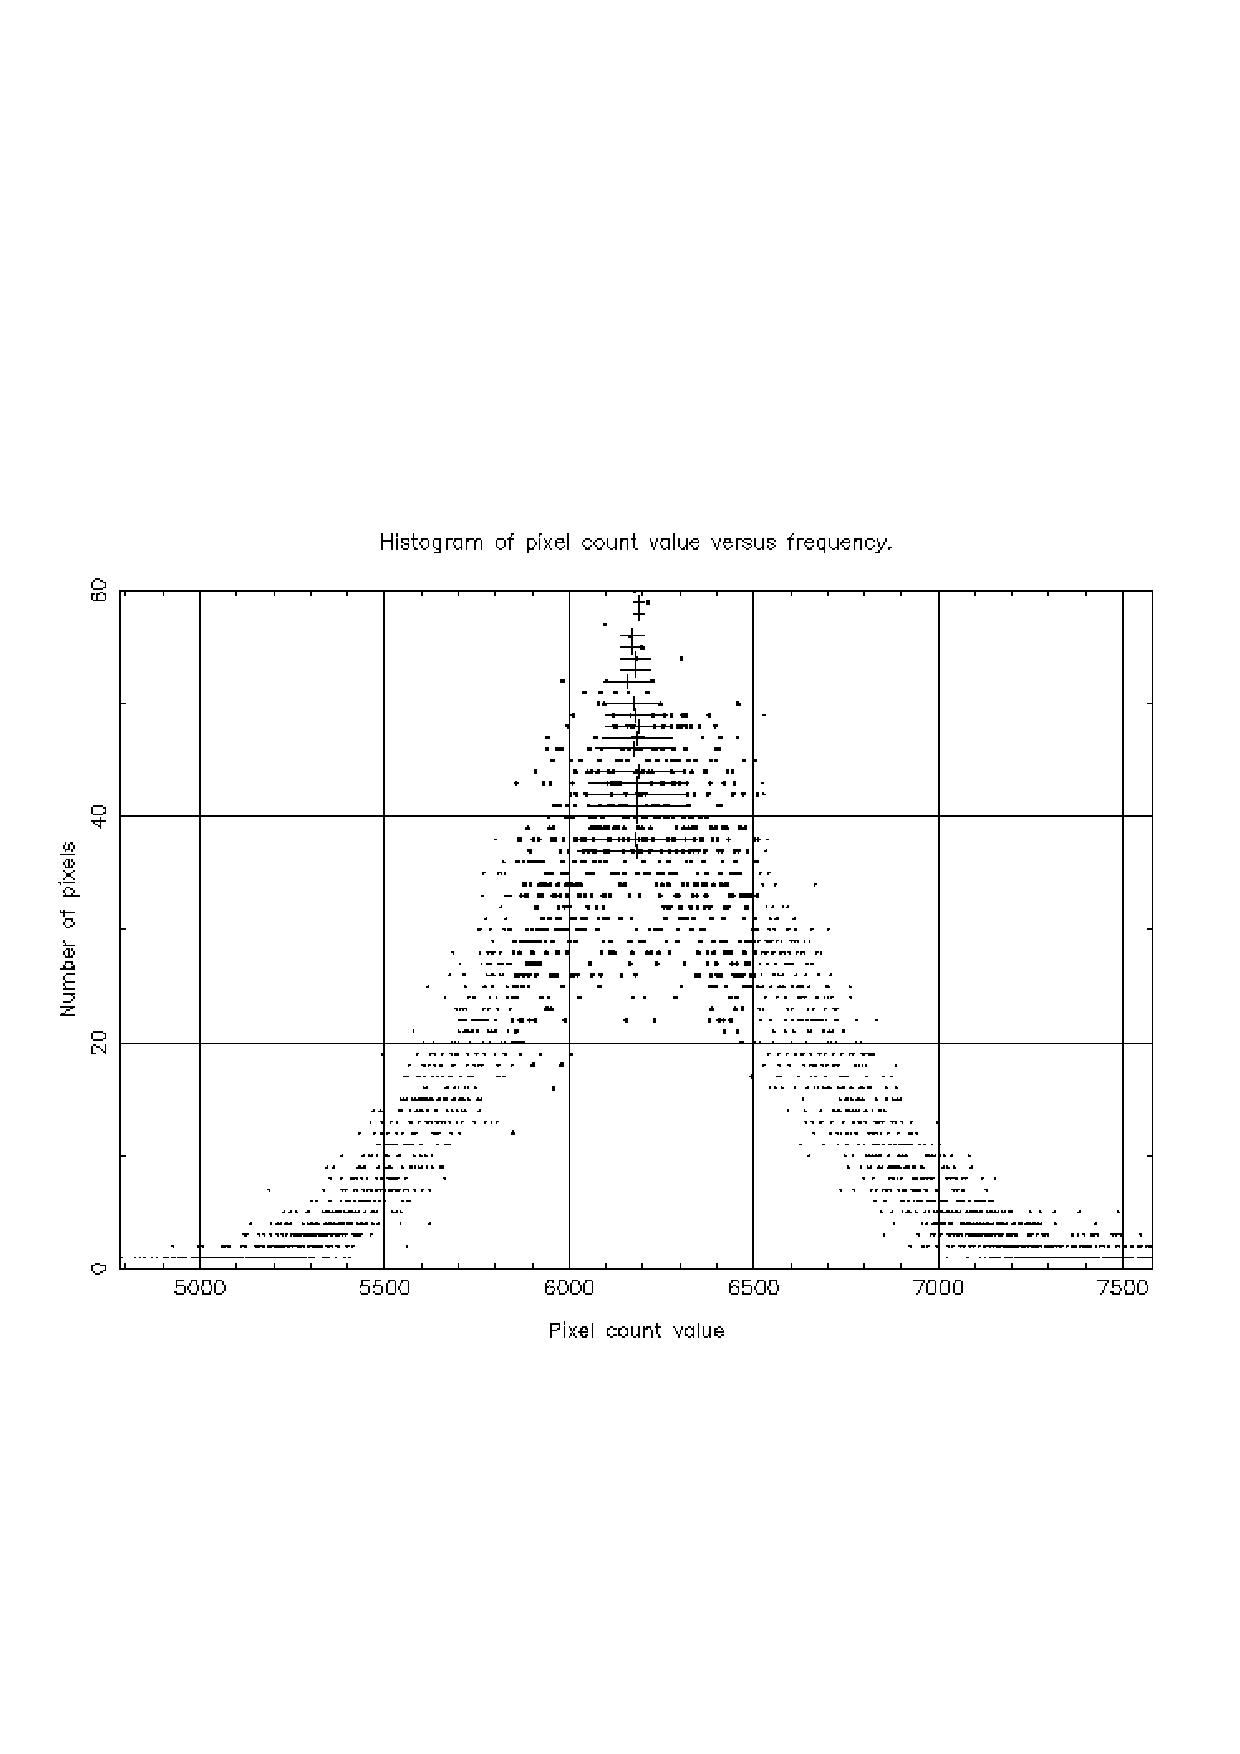
\includegraphics[width=151mm,height=100mm]{sun180_diag1}
\caption{The unsmoothed pixel count histogram generated by HISTPEAK.}
\end{figure}

If you re-run HISTPEAK but this time input an SFACT value of 4 you will find
that the results for some quantities are different. This is as you would
expect when histograms are smoothed. As you can see from the excerpt below,
the values affected are those relating to values extracted from the
smoothed histogram. Figure 2 shows the histogram and the effect
of smoothing upon the shape of the pixel count distribution - smoothed
points are plotted bold.

\newpage
\begin{terminalv}
Histogram modal values:
Unsmoothed:              6179.000     Smoothed:             6176.000
Projected:               6175.306     Interpolated:         6193.840

Absolute dev.:            333.494     Variance:              183890.
Standard. dev.:           428.824     Back. st. dev.:        365.752

Smoothing filter radius:
Radius request:                 4     Radius actual:               4

Contents of the most occupied histogram bin:
Unsmoothed:                60.000     Smoothed:               46.204
Interpolated:              39.609
\end{terminalv}

\begin{figure}[htb]
\centering
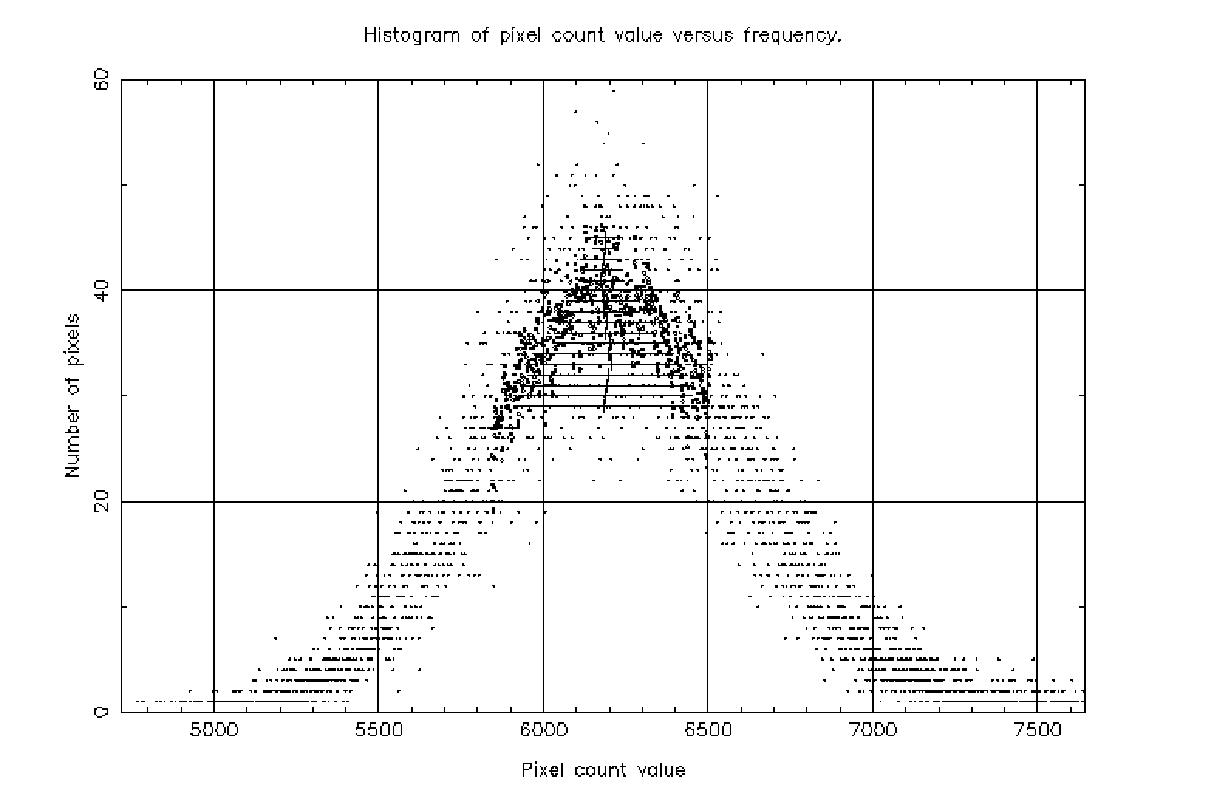
\includegraphics[height=100mm,width=150mm]{sun180_diag2}
\caption{The smoothed pixel count histogram generated by HISTPEAK.}
\end{figure}

\subsection{Session 2 --- Interactive profiling by intensity analysis}
\xlabel{SESSION2}

One of the key uses of ESP is for profiling images of galaxies.
The ESP application for doing this is ELLPRO. If we again assume we
are logged on and that the \texttt{esp} command has been issued,
then the following is a simple session using it. The example
assumes also, that the \texttt{kappa} command has been issued allowing use of the
\xref{DISPLAY}{sun95}{DISPLAY} routine. For the simplest use of ELLPRO, the image containing
the galaxy to be profiled needs to be displayed.

\begin{terminalv}
% display in=ic3374c mode=faint device=xw
% lutgrey device=xw
\end{terminalv}

The first instruction clears the X window and displays the NDF image file
ic3374c. The second instruction defines
the colour table to be employed for that window.

The next step is to start up ELLPRO and give it information about how
you wish to work.

\begin{terminalv}
% ellpro

ESP ELLPRO running.
MODE - Use the application interactively? /TRUE/ > Y
CURSOR - Use the cursor to identify the galaxy centre? /TRUE/ > Y
\end{terminalv}

Choosing a value of TRUE for MODE tells the program that you will
either be typing in a value for the location of the galaxy centre on the image
or using a cursor to indicate where it is. The alternative is for the program to
read in a list of co-ordinates from a text file. Specifying a value of TRUE
for CURSOR then tells the program that you will be inputting the location by
using a cursor. This is only possible if you have previously displayed an
image on a device and it is still visible. If several images are currently
displayed on a device then the most recently added image displayed
(containing a DATA component) is examined. This information is obtained from
the AGI database.

The next information required is the
name of the display device on which your galaxy is currently displayed --
in this case Xwindows. It then looks at the AGI database to determine
what image you used to create the displayed image and displays its name
to allow you to check that it is the right one. After a brief pause
(duration depends on your hardware) the cursor may be used to identify the
centre of the galaxy. How this may be done differs slightly from device type to
device type. However, it is by use of buttons on an Xwindow and by use
of the space bar and buttons on IKONs.

\begin{terminalv}
IMGDEV - Which device is displaying the image? /@xwindows/ > xw

Using /local2/data/esp/ic3374c as the input NDF.

Select the centre of the galaxy to be profiled.
Keyboard "2" key:   Quit the program.
Keyboard "." key:   Select the galaxy.
Keyboard "1" key:   Show the cursor co-ordinates.
  SKY frame co-ordinates:  RA = -11:23:21.6,  Dec = 62:13:07
\end{terminalv}

When you identify the location you want,
the program reports that location in the Current co-ordinate
system of the image, which in this case is SKY,
with co-ordinates of RA and Dec.
Information about co-ordinate systems associated with an NDF file is held
in its WCS (World Co-oordinate System) component.
Briefly, the WCS component contains several co-ordinate \emph{frames},
allowing positions within the data array to be addressed in different ways.
Each frame has a label, called its \emph{Domain}, which usually describes
the co-ordinate system; two important ones are GRID (which is
always present) and SKY (which may or may not be).
At any given time one of these frames is designated the \emph{Current\/} one,
and this determines the co-ordinates used when positions are requested
or reported by ESP or other Starlink packages like \xref{KAPPA}{sun95}{}.
You can change between frames using KAPPA's
\xref{WCSFRAME}{sun95}{WCSFRAME} command.
For instance the following would cause all positions to
be reported in PIXEL co-ordinates instead:
\begin{terminalv}
% wcsframe ic3374 pixel
\end{terminalv}
To find out more about WCS components see \xref{SUN/95}{sun95}{se_wcsuse}.

Once the galaxy centre is identified, it is necessary to describe how far out
from the centre you want the profiling to continue (if possible). This is again
achieved via the cursor.

\begin{terminalv}
Indicate the outer limit of the galaxy.
Keyboard "2" key:   Quit the program.
Keyboard "." key:   Select the outer limit of the galaxy.
Keyboard "1" key:   Show the cursor co-ordinates.
  SKY frame co-ordinates:  RA = -11:23:17.0,  Dec = 62:12:43
\end{terminalv}

When this has been done, a circle is drawn around the galaxy showing the extent
of the profiling requested. This may, or may not, be visible depending on the
colour of the image background. However, this can be overcome by use of the
command line parameter COLOUR when starting ELLPRO, i.e.:

\begin{terminalv}
% ellpro colour=n
\end{terminalv}

Where the valid range of colours (N) for drawing the lines is 0--3.

The next prompts displayed are simple to understand.

\begin{terminalv}
FRZORI - Is the galaxy origin to be frozen? /FALSE/ > F
BACK - Background value /6179/ > 760.5
SIGMA - Standard deviation of the background /392/ > 12.07
Using info from SKY frame - pixels are  0.961 arcseconds square.
\end{terminalv}
The first parameter, FRZORI,
asks if the galaxy position you proposed (and refined with
AUTOL if required) should be held to
be the galaxy centre throughout the profiling operation or,
is it allowed to vary slightly
from ellipse to ellipse if that provides a better fit?
BACK and SIGMA are the modal pixel value in the image and its
associated standard deviation.
Since the image in this example has a SKY co-ordinate frame
(it does not have to be the Current frame),
the program then works out the pixel size in arc seconds and reports it.
If your image does not have any SKY co-ordinates, then you will
be prompted to enter this as the value of a parameter PSIZE.
The final group of configuration parameters is as follows:
\begin{terminalv}
ZEROP - Surface brightness zerop point (in magnitudes per arcsec) /27.5/ >
AUTOL - Automatically search for better origin? /YES/ > yes
AUTOLT - Use a centroid? /NO/ > yes
ARDFIL - Masking ARD file /@ardfile.dat/ > !
!! SUBPAR: Null (!) response to prompt for parameter ARDFIL
WARNING! - ARD file not used.
\end{terminalv}
ZEROP is the base of the scale for the surface brightness plot
which will be made.
AUTOL will refine
the estimate of the galaxy centre position you have proposed with the cursor
if set to TRUE. In the case shown it has been requested and the method
chosen was a centroid.
The last information required is to name an ARD file if one is to be used to
define the good parts of the image. In this case `!' is entered because no
ARD file will be used. Instead, the whole image will be used. To make sure
you're aware of this, the program issues a warning.

It should be noted that for those required inputs which match the
values suggested by the program, it is sufficient just to press
the Return/Enter key to accept the proposed value.

The program then starts to work on the profiles. It first makes a guess at
the crude shape of the galaxy at some smallish radius and (hopefully)
sensible S/N ratio and displays this.
Next, it makes a full estimate of the profile at that radius before dropping
down to smaller radii and then increasing upward again until
one of the profiling limits (see LIM1, LIM2 and RLIM in Appendix
\ref{des:ELLPRO})
is exceeded. Results of the
profiling activity are displayed as they are calculated. This is done to allow
you to see what progress is being made.

\begin{small}
\begin{terminalv}
Initial parameter estimates
Rad(a)     5.41  Posang   12.1  1/Ellipt.  .692

  X       Y     Points   Rad(a)    Count     PA  1/Ellip Dev.  PPU  Statistic

Residual calculation: weighted SD
  93.3    96.5    76      4.81      114.2  -16.4  0.593    0.9  100.  0.87E+03
  93.0    96.1    20      0.16      213.8  -31.7  0.116    0.4  100.  0.97E+03
  93.0    96.2    20      0.27      211.6  -23.4  0.141    0.9  100.  0.97E+03
  93.0    96.1    20      0.36      211.3  -23.4  0.141    0.8  100.  0.97E+03
  92.9    96.2    20      0.45      210.6  -23.4  0.141    0.8  100.  0.97E+03
  ----    ----    ---     ----       ---    ----  -----    ---  ----
  ----    ----    ---     ----       ---    ----  -----    ---  ----
  ----    ----    ---     ----       ---    ----  -----    ---  ----
  93.5    95.8   332     19.93        1.9   -2.9  0.602    0.5   92.  0.76E+03

Mean count below threshold LIM2.
\end{terminalv}
\end{small}

Descriptions for the headings may be found in Appendix~\ref{app:outputfiles}.

When the application has finished profiling the galaxy it issues a message
indicating why the profiling action was stopped.

You are then prompted for the name of a device on which the image should be
displayed. This is done by first asking you if the device currently displaying
the image is to be used
and then, if you say no, asking for the name of the new device. In the event
that you request the current device as the place the profile results should be
displayed, you will be further prompted to indicate (using the cursor) in which
quadrant of the
screen it is to be shown. It must be remembered that any objects in that part
of the screen will, subsequently, be obscured, as may be seen in Figure 3.

\begin{terminalv}
SAME - Use the same graphics device for the results graph? /TRUE/ > f
DEVICE - Which device/type to display the graph /@x2windows/ >

OUT - Text file for profile output /@elp/ > testprof.dat
AGAIN - Profile again? /FALSE/ >
\end{terminalv}

\begin{figure}[htb]
\centering
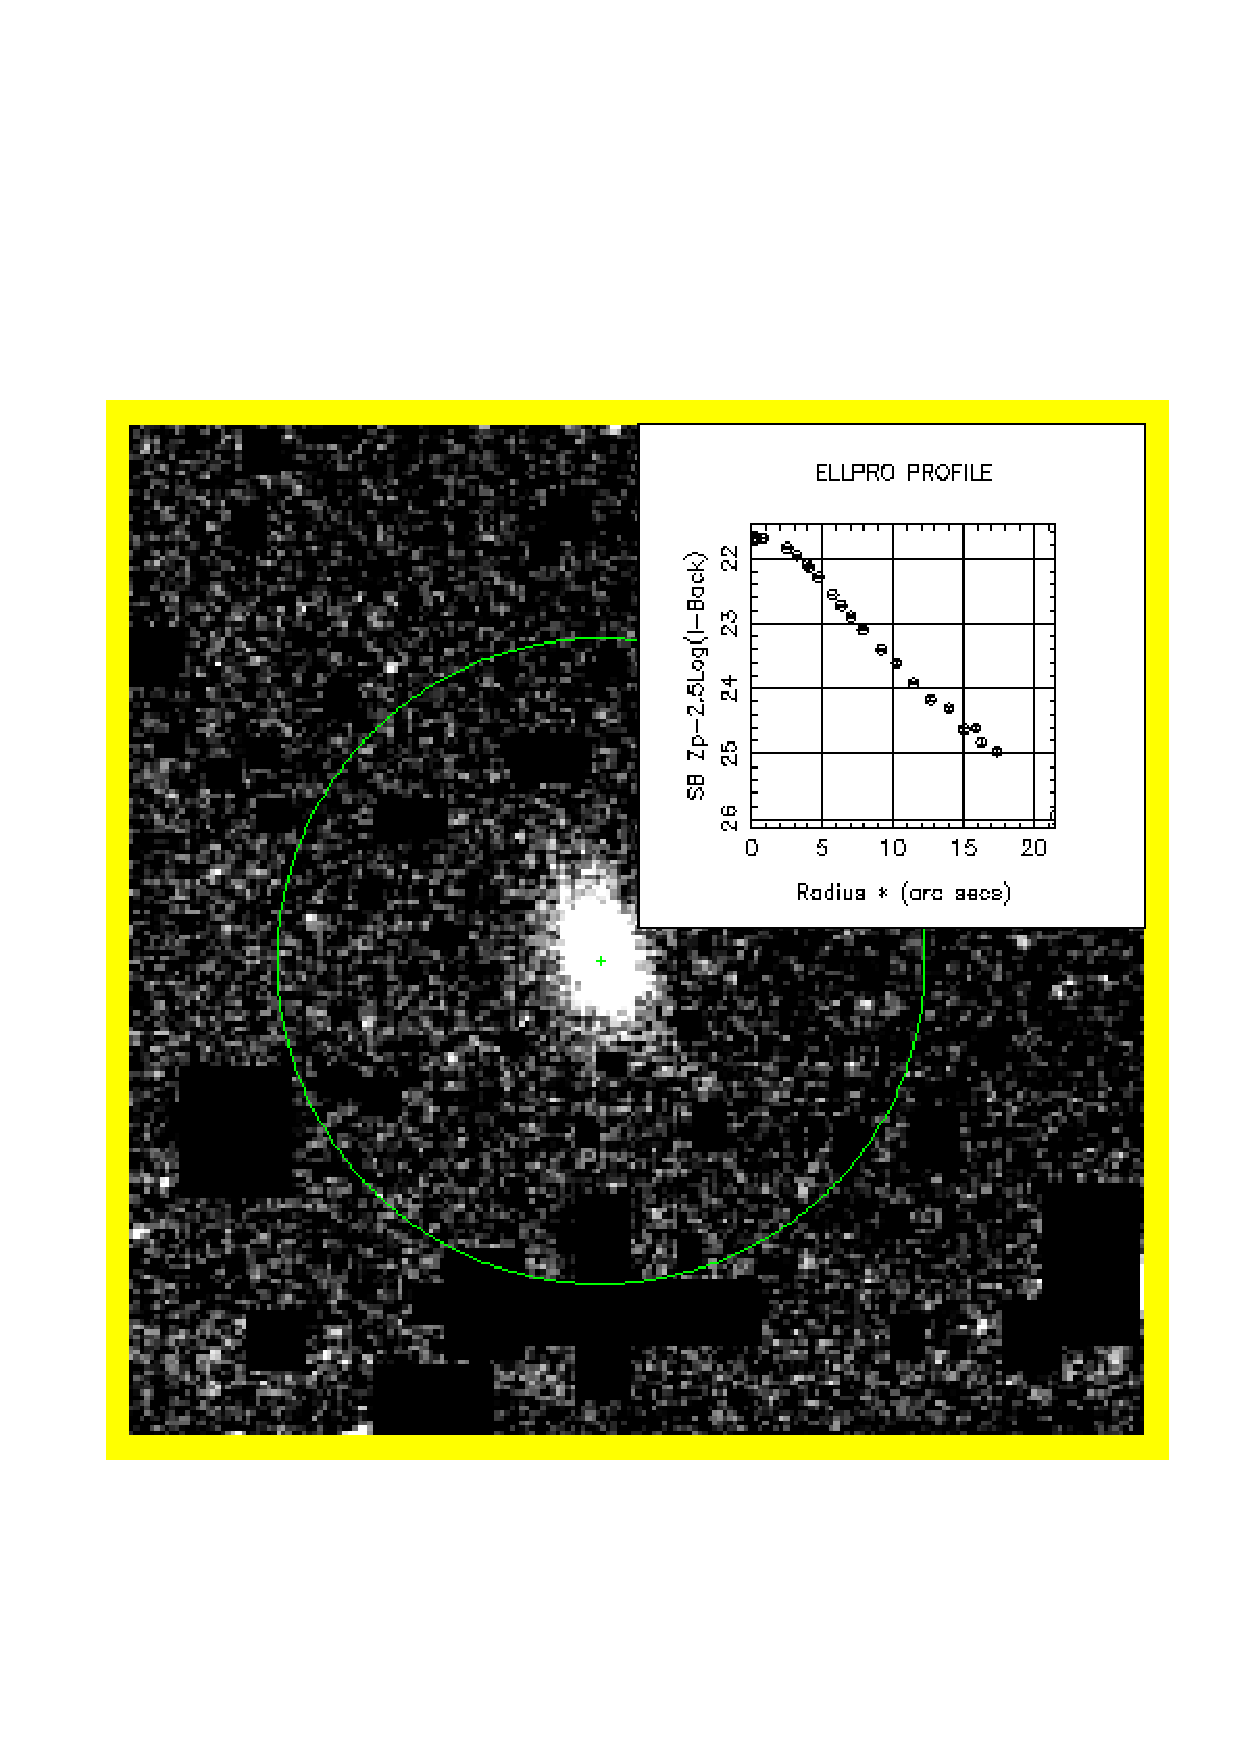
\includegraphics[height=125mm,width=125mm]{sun180_diag3}
\caption{The galaxy image and profile when displayed on the same device.}
\end{figure}

You are also prompted for the name of an output file into which the
profiling results are to be placed. If it is found that the name you provide is
not allowable (e.g.\ there are illegal characters in the name or the file named
already exists) you will be reprompted. A `!' may be used to avoid creating a
file if you do not wish to retain a copy of the results.

Finally you will be asked if you wish to try again. If you answer yes, the
program will go back to the point at which you identified the location of the
galaxy centre on the image and start again. Where possible, you will not be
reprompted for input you have already provided.

You will find that the ESP ELLFOU application works in a very similar manner.
Consequently, you are now in a position to profile galaxies
interactively and to generate profiles using either intensity (ELLPRO) or
contour analysis (ELLFOU).


\subsection{Session 3 --- File based profiling by intensity analysis}
\xlabel{SESSION3}

Session 2 showed how one or more galaxies on an image might be
processed interactively to yield their profiles. However, there are
times when you want to profile virtually every object in an image.
This can be done using ELLPRO or ELLFOU in essentially the same manner.
The only difference is that you supply the image co-ordinates of the galaxies
you want profiled in a text file. Such a file may be easily created
using the LOGFILE option of \xref{KAPPA}{sun95}{}'s CURSOR or by taking
information from a file generated by object identification software such as
\xref{PISA}{sun109}{}.

The file used in the example below, contains the following:

\begin{terminalv}
426.8958 155.2692
278.7055 299.9713
206.613 350.2151
\end{terminalv}

The columns represent the $x$ and $y$ co-ordinates respectively. A third column
might also have been included, giving a value for the background to be
used for each of the galaxies. In the absence of a third column, the image's
global value is employed. Local background values for different points may be
easily determined using the ESP LOBACK application.

The co-ordinates given in this file should be in the
Current co-ordinate system of the image (which can be selected by
\xref{WCSFRAME}{sun95}{WCSFRAME} as described in the previous section),
so that for instance if the image had the SKY frame as Current,
a suitable file might read something like:

\begin{terminalv}
 0:07:21.4   30:33:04
 0:07:42.6   30:32:10
 0:07:22.9   30:27:20
\end{terminalv}

An example of the sort of input required is shown below.

\begin{small}
\begin{terminalv}
% ellpro

ESP ELLPRO running.
MODE - Use the application interactively? /TRUE/ > f
INFILE - Text file containing co-ordinates /@coords.dat/ > f5coords.dat
IN - Image NDF filename /@ic3374c/ > f5flat
FRZORI - Is the galaxy origin to be frozen? /FALSE/ >
BACK - Background value /760/ > 22712
SIGMA - Standard deviation of the background /12/ > 57
PSIZE - Size of the pixels (in arcsec) /1/ > 1
RLIM - Maximum ellipse radius (in pixels) /10/ > 40
ZEROP - Surface brightness zerop point (in magnitudes per arcsec) /27.5/ >
AUTOL - Automatically search for better origin? /TRUE/ >
AUTOLT - Use a centroid? /TRUE/ > f
Default background used for object at  426.9,  155.3
Default background used for object at  278.7,  300.0
Default background used for object at  206.6,  350.2
ARDFIL - Masking ARD file /@ardfile.dat/ > !
WARNING! - ARD file not used.
OUT - Text file for profile output /@testprof.dat/ > f5results.dat

Working on PIXEL co-ordinates: 426.9  155.3
  19 ellipses determined.
Working on PIXEL co-ordinates: 278.7  300.0
  30 ellipses determined.
Working on PIXEL co-ordinates: 206.6  350.2
  12 ellipses determined.
\end{terminalv}
\end{small}

Note that since the image in this example does not have a SKY
frame in its World Coordinate System component,
you have to enter the PSIZE parameter by hand.

In the example given, the co-ordinates file coords.dat identified the
locations of 3 galaxies, but it could just as
easily have contained information on many more. The current
upper limit imposed by ESP is 10000.


\subsection{Session 4 --- Obtaining galaxy pieslice cross-section}
\xlabel{SESSION4}

The ESP application SECTOR may be used to interactively derive a
pieslice cross-section of a galaxy. Before it may be used the
NDF image containing the galaxy must be displayed on a suitable
display device. This may be done in a manner similar to
that described in Session 2. Once the image is displayed, SECTOR
may be run.

The first prompt you are faced with asks if you are going to use a cursor
to define the position of the galaxy centre and to describe the
direction, size and length of the pieslice. If you answer FALSE to this query,
you will have to input all your values via the keyboard. However, it is much
simpler to use a cursor, as in the example below.

\begin{terminalv}
% sector

ESP SECTOR running.
CURSOR - Use the cursor to identify the galaxy centre? /TRUE/ >
IMGDEV - Which device is displaying the image /@xwindows/ >
\end{terminalv}

You are then asked
on what device the image to be examined is displayed (DEVICE).
SECTOR then examines the AGI image database to determine the image's name.
This is displayed so that the you can be sure the image used is as expected.

Control then passes to the cursor and you are prompted to use the
cursor (and/or the keyboard) to identify the part of the image to be used in
the pie-slice cross-section.

\begin{terminalv}
Using /local2/data/esp/ic3374c as the input NDF.

Select the centre of the galaxy.
Keyboard "2" key:   Quit the program.
Keyboard "." key:   Select the galaxy.
Keyboard "1" key:   Show the cursor co-ordinates.
  SKY frame co-ordinates:  RA = -11:23:21.7,  Dec = 62:13:07

Indicate centre of the outer limit of the sector.
Keyboard "2" key:   Quit the program.
Keyboard "." key:   Select centre of the outer  limit of the sector.
Keyboard "1" key:   Show the cursor co-ordinates.
  SKY frame co-ordinates:  RA = -11:23:21.4,  Dec = 62:12:25

Select the sector angular width.
Keyboard "2" key:   Quit the program.
Keyboard "." key:   Select width of the sector.
Keyboard "1" key:   Show the cursor co-ordinates.
  SKY frame co-ordinates:  RA = -11:23:23.6,  Dec = 62:12:27
\end{terminalv}

The application then asks
for information about the image (BACK, SIGMA and, if necessary, PSIZE),
how the results are to be displayed (SURF, RADISP, ZEROP)
and where the results are to be displayed (SAME, DEVICE).

\begin{terminalv}
MIRROR - Use two diametrically opposite slices? /TRUE/ > TRUE
BACK - Background count value /760.5/ >
SIGMA - Standard deviation of the background /12/ >
Using info from SKY frame - pixels are  0.961 arcseconds square.

SURF - Display counts as surface brightness? /TRUE/ > TRUE
RADISP - Radius display mode /'r'/ > r
ZEROP - Surface brightness zerop point /27.5/ >
AUTOL - Automatically search for better origin? /TRUE/ >
ARDFIL - Masking ARD file /@ardfile.dat/ > !
!! SUBPAR: Null (!) response to prompt for parameter ARDFIL
WARNING! - ARD file not used.
SAME - Use the same graphics device for the results graph? /TRUE/ > f
DEVICE - Which device/type to display the graph /@x2windows/ >
\end{terminalv}

The RADISP and SURF options above specify that the `profile' will be displayed
in the form of surface brightness versus linear radius. Other options exist for
displaying the mean pixel count versus radius transformed into its
logarithm, square root or quarter power.

AUTOL set to TRUE means that the application will look at the parts of the
image immediately surrounding the galaxy centre suggested
and, if possible, will identify a better candidate. In the instance given
AUTOL has been used.

The option MIRROR allows for the pieslice
defined to be duplicated on the other side of the galaxy
origin. This effectively increases the signal since more of the image will be
sampled, but is only really applicable when the image is roughly
symmetrical. Figure 4 shows the selected sector displayed on the galaxy. It
also shows the mirror image sector generated by the MIRROR parameter being
set to TRUE.

The graph is then displayed and you are asked to indicate (using the cursor)
the radius range of the profile points to be used to calculate the scale
lengths.

\begin{terminalv}
Select a point defining the lower radius limit.
Keyboard "2" key:   Quit the program.
Keyboard "." key:   Select lower radius limit.

Select a point defining the upper radius limit.
Keyboard "2" key:   Quit the program.
Keyboard "." key:   Select upper radius limit.
\end{terminalv}

The graph then displays the galaxy profile `fits' and the
results of the scale length calculations are printed, showing
values for the central surface brightness of the galaxy for both elliptical
and spiral galaxy models.

\begin{figure}[htb]
\centering
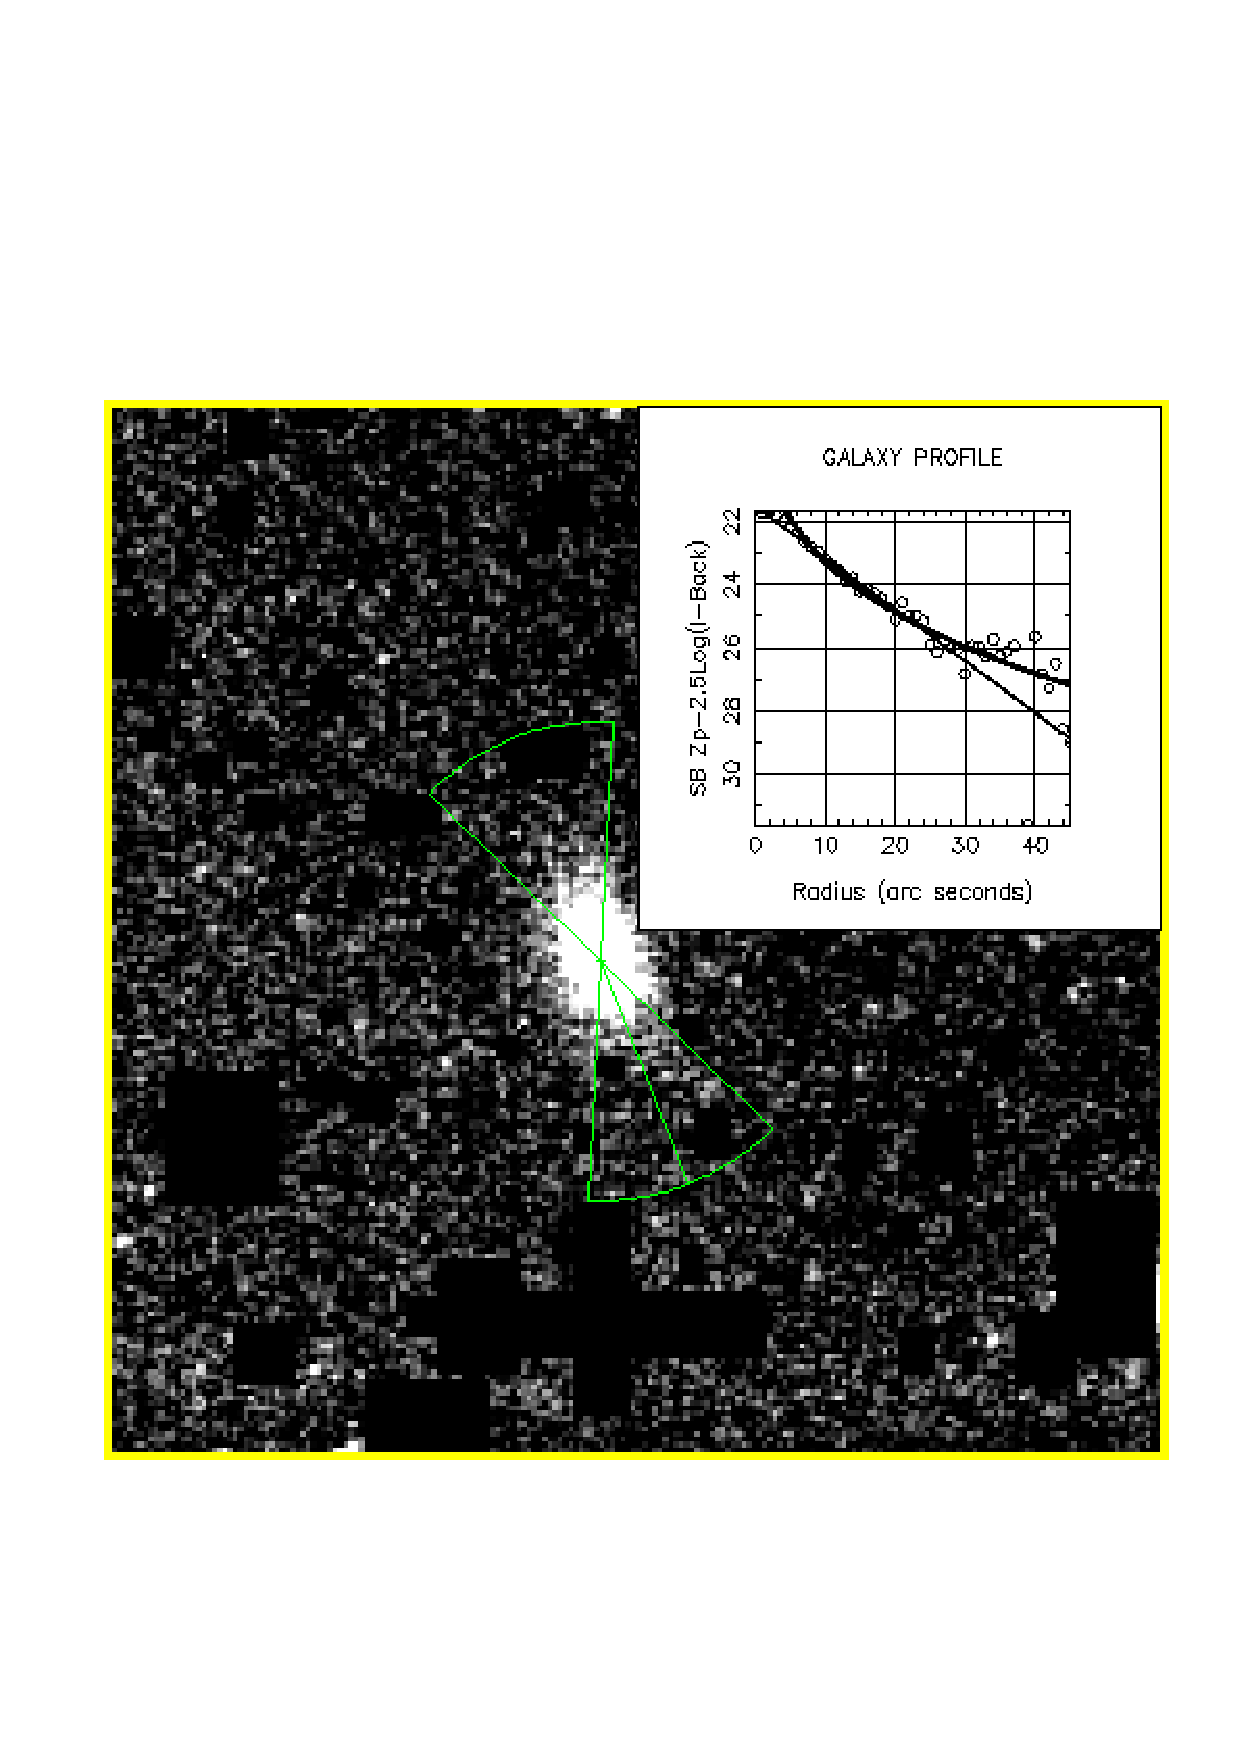
\includegraphics[height=125mm,width=125mm]{sun180_diag4}
\caption{The galaxy image, showing the sector area sampled and profile.}
\end{figure}

\begin{terminalv}
SECTOR Results for file: /local2/data/esp/ic3374c

Origin:  -11:23:21.6  62:13:08

Pixel count (raw):              980.00
Pixel count (subtracted):       219.50
Pixel count (sigma):             18.29
Pixel count (Log(I-BACK)):        2.34
Mag. rel. zero point:          21.6464

Central mag. spiral:  21.4506
Central mag. ellipt:  16.9384
Above or below sky:   -0.5397

Number of data points:      46 ie.  43.22"
Range used (arc sec):     0.63,  26.88

Points used for spiral calculation:        27
Scale length spiral:                   6.2582
Points used for elliptical calculation.:   27
Scale length elliptical:              0.08769
\end{terminalv}

Finally, you are given the chance to obtain a pieslice of some other
part of the image.

\begin{terminalv}
OUT - Text file for profile output /@sectout.dat/ >
AGAIN - Profile again? /FALSE/ >
\end{terminalv}


\subsection{Session 5 --- Examining profiling results}
\xlabel{SESSION5}

The applications ELLPRO, ELLFOU and SECTOR all generate text output
files that may be examined using the application GRAPHS. This lets
you display graphs such as surface brightness, ellipticity or position
angle versus radius (or some transformation thereof). GRAPHS
has been made as simple to use as possible. A simple session is shown below.
The input file used (\texttt{prof.dat}) was generated by ELLPRO.

\begin{terminalv}
% graphs

ESP GRAPHS running.
MODE - Use the application interactively? /TRUE/ > true
CURSOR - Use the cursor? /FALSE/ > false
INFILE - Name of ESP data file /@test.dat/ > prof.dat

OUT - Text file for profile output /@graphs.out/ >
\end{terminalv}

By opting for MODE to be TRUE, you have opted to interactively examine
each of the profiles from the input file in turn. In this mode, the profiles are
displayed (if required) on a graphics device and you must
identify the radius range of the data points to be used to determine the
galaxy scale length. CURSOR set to FALSE means that the radius range will
either be typed in or GRAPHS will automatically guess at an
appropriate range to use. The inputs INFILE and OUT identify the input and
output text files respectively. The graphical output is shown in
Figure 5.

\begin{terminalv}
ELLPRO Header found.
Source image was: f5flat
End of filename report.

WHATD - Parameter to display /'s'/ > s
RADISP - Radius display mode /'q'/ > r
DEVICE - Which device/type to display the graph /@xw/ > xw
RRANGE - Automatic radius limit selection? /TRUE/ > f
FITLIM - Limit of the radius range to be fitted (in arcsec) > 2.5,15
\end{terminalv}

\begin{figure}[htb]
\centering
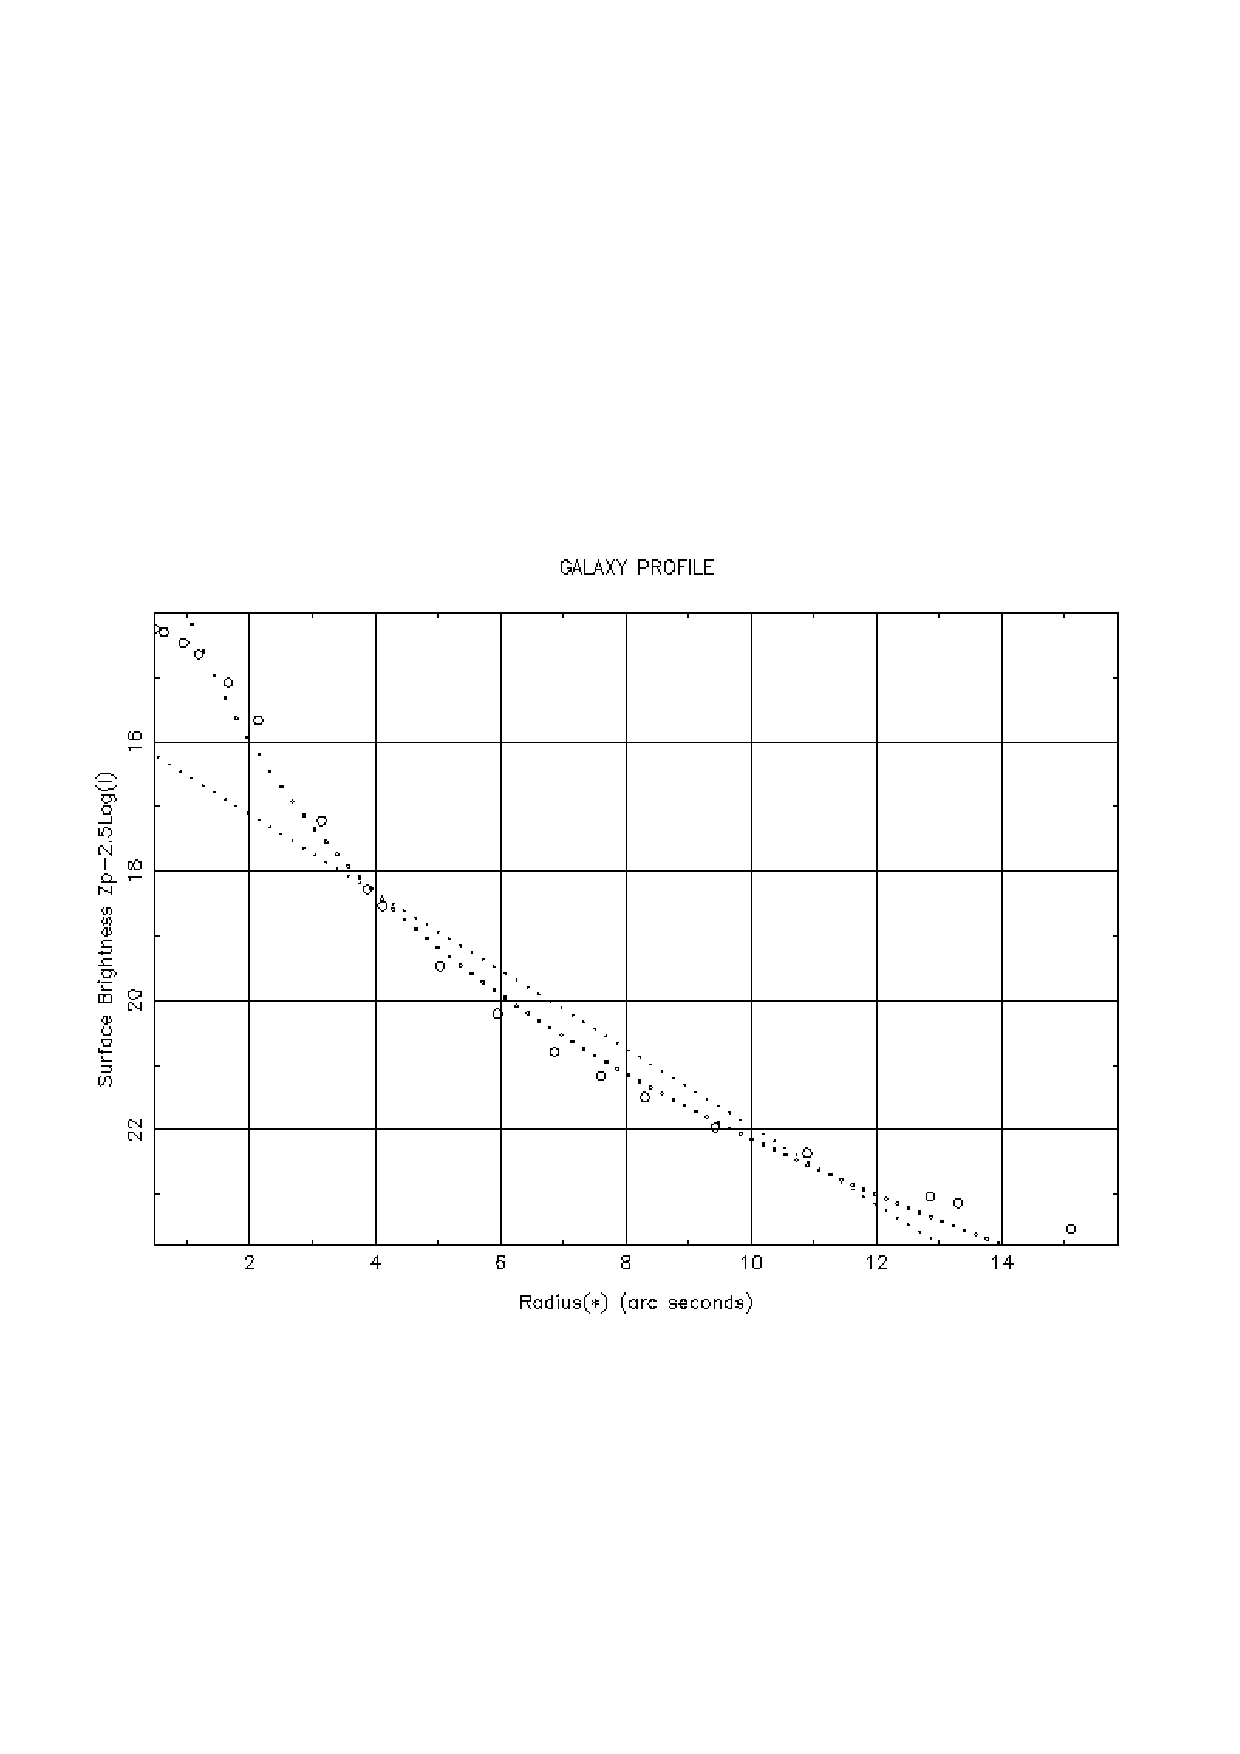
\includegraphics[height=100mm,width=150mm]{sun180_diag5}
\caption{The galaxy profile with elliptical and spiral models shown.}
\end{figure}

GRAPHS shows you the name of the application that generated the
profile you are examining and the name of the image from which
it was derived. It then asks you to define what is to be displayed.
WHATD set to `s' means surface brightness will be displayed against
linear radius (defined by RADISP set to `r'). DEVICE again defines the
name of the graphics device to be employed while RRANGE and FITLIM define the
radius range of the part of the profile to be fitted.

\begin{terminalv}
Number of data points:      19
Range used (arc sec):     2.5,  14.75
X and Y co-ordinates (Base):  89.3, 99.8
X and Y co-ordinates (Current):  1787.8, 698.3
\end{terminalv}

Two sets of co-ordinates are displayed here to identify the point
in question: those of the Base frame (GRID co-ordinates, which
always start at (1,1) for the bottom left pixel in the image)
and those of whatever was the Current frame when the
file being plotted by GRAPHS was generated.
If the Current co-ordinate frame of the image has been changed
using \xref{WCSFRAME}{sun95}{WCSFRAME} then the Current co-ordinates
will no longer be correct, but the Base frame ones always will.
You can set the Base frame to be Current,
and so used for display etc.,
at any time by doing
\begin{terminalv}
% wcsframe myimage grid
\end{terminalv}

More information is then given;
values for central surface brightness (CSB), scale length and
range of data points used are displayed. The LCC (linear correlation
coefficient) values give an idea of how good the fit was. Finally, you are
given the option to try fitting the profile again. If there is only one
object in the input file, the application will then stop, otherwise the
next profile from the file will be read and you will be allowed to profile
that.

\begin{terminalv}
Points used for spiral calculation:        12
Scale length spiral:                   2.0442
Points used for elliptical calculation.:   12
Scale length elliptical:              0.00183
Extrapolated CSB spiral:              16.6
Extrapolated CSB elliptical:           4.6
Spiral LCC squared:                    .92
Ellip. LCC squared:                    .95

AGAIN - Display again? /TRUE/ > f

End of file found.
\end{terminalv}

One detail of this example needs a little more explanation. In one
of its modes, GRAPHS can work automatically on input files
containing information on lots of galaxies without further
input. This means that GRAPHS can take the file generated in Session
3 (containing the profiles of three galaxies) and determine from them,
values for the central surface brightness and scale length.
This method of working is selected by setting MODE to FALSE, but otherwise
differs only slightly from the example above.



\subsection{Session 6 --- Looking at the image background variation}
\xlabel{SESSION6}
In this  session, the ESP application SKEW is employed to show
what parts of a source image suffer from poor flat fielding.
Before you run this program you should run HISTPEAK for the source image to
determine its background value and also its associated standard deviation.

Then, the session will go something like this:

\begin{terminalv}
% skew

ESP SKEW running.

IN - Image NDF filename /@skew/ > cnt4141c
Filename:   cnt4141c
Title:      Source Image
Shape:      525 x 520 pixels
Bounds:     x= 1:525  y= 1:520
Image size: 273000 pixels
OUT - Output NDF filename /@skew/ > skew
WIDTH - Template width (in arcsec) /8/ >
PSIZE - Pixel size /1/ > .88
MODET - Use a global mode value (y/n)? /YES/ >
BACK - Background sky value /6200/ > 22716
USEALL - Include very bright pixels (y/n)? /NO/ >
SIGMA - Standard deviation of the image pixels /390/ > 56
NSIGMA - Level of the cutout in SIGMA /10/ >
MULT - Output skewness multiplying factor /1000/ >
\end{terminalv}

The parameters IN and OUT refer to the source image and the output image
respectively. BACK, SIGMA and PSIZE all relate to the image
cnt4141c.

When the MODET option is set to FALSE, SKEW calculates a local background
value when determining the skewness of each part of the image. In this
example it is set to TRUE, so the image's global background value is used
instead. This is the faster option.

USEALL and NSIGMA are used to define a pixel count cutoff value. If one of the
image pixels is brighter than the global background (BACK) plus a certain
number (NSIGMA) of background value standard deviations (SIGMA) it is excluded from the
calculations. This may be used to reduce the influence of cosmic rays and
other bright image features which might otherwise dominate the output.

Since skewness values are usually fairly small, a multiplying factor may be
applied to all the skewness values calculated. This is specified by MULT.

Finally, SKEW shows you what it is currently doing and how
far it has got. This is because, for large images, it can
take a considerable time to run, especially, if the template size is large.

Figure 6 shows a source image and the image generated by SKEW when it was sampled
over boxes approximately 10x10 pixels in size. Note how the previously
unnoticed bad column (slightly left of centre near the top) is easily spotted
and how large the full extent of the poor flatfielding is.

\begin{terminalv}
Applying SKEW to file: cnt4141c
Results file will be:  skew
Global background value used.
High count cutoff was used.

Percentage done so far: 10
Percentage done so far: 20
Percentage done so far: 29
..........................
..........................
Percentage done so far: 98
\end{terminalv}

\begin{figure}[htb]
\centering
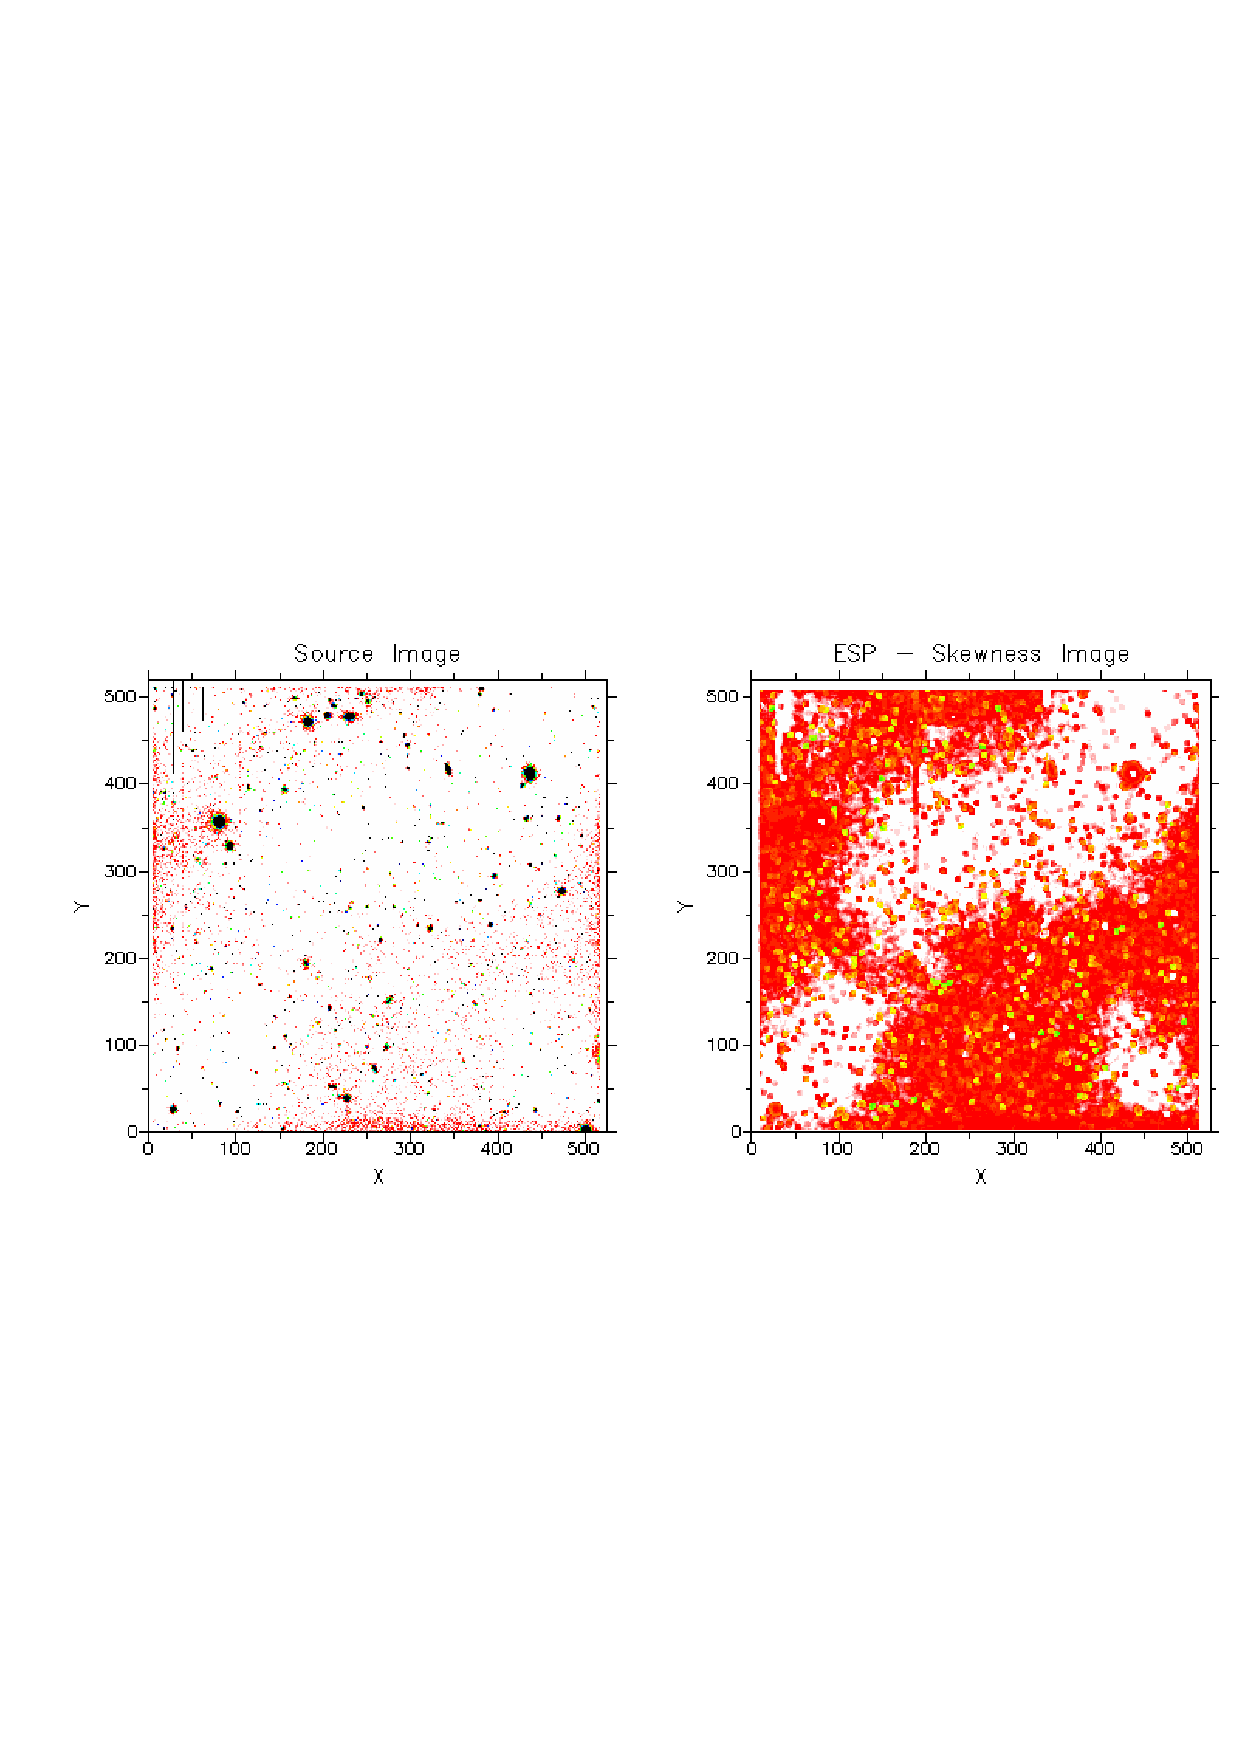
\includegraphics[height=75mm,width=150mm]{sun180_diag6}
\caption{A poorly flatfielded source image and the output generated by SKEW.}
\end{figure}

\subsection{Session 7 --- Interactively obtaining 2-D Gaussian source profiles}
\xlabel{SESSION7}
In some of the earlier sessions you saw how to profile a galaxy in
terms of an ellipse using ELLPRO and ELLFOU. Sometimes in astronomy
it is useful to profile a source (or sources) in terms of 2-D Gaussian
functions, this is especially useful for users of JCMT data (see also
\xref{JCMTDR}{sun132}{}). In ESP this operation is performed by the
application GAUFIT.

GAUFIT is similar to ELLPRO, SECTOR and ELLFOU in that it may be operated
using a cursor or a simple text file to select the source position(s) that
must be examined.

GAUFIT now contains two distinct fitting algorithms: the original one,
which obtained the fit parameters by hunting through a region of
parameter space constrained by you, and a new one (as of version 0.9),
which uses a non-linear least-squares algorithm to obtain the
parameters and their uncertainties.  For further details on the new
algorithm, see the detailed description of GAUFIT in
section~\ref{des:GAUFIT}.  The interface has not changed radically,
but I will show two complete examples below.







\subsubsection{GAUFIT: original fitting algorithm}

Once the image to be analysed has been examined using
HISTPEAK and displayed using \xref{KAPPA}{sun95}{}'s DISPLAY, an interactive
session might proceed as follows:

\begin{terminalv}
% gaufit

ESP GAUFIT running.

MODE - Use the application interactively? /TRUE/ >
COLOUR - Pen colour? /1/ >
ANGCON - Use clockwise positive rotation convention? /FALSE/ >
ANGOFF - Position angle offset /0/ >
IMGDEV - Which device is displaying the image? /@xwindows/ >

Using /local1/export/home/norman/s/src/esp/ic3374c as the input NDF.

Select the source location
Left mouse button:        Select location.
Middle mouse button:      Show cursor coordinates.
Right button or CTRL-C:  Quit selection.

  SKY frame co-ordinates:  RA = -11:23:21.4,  Dec = 62:13:07

Indicate the outer limit of the source.
Left mouse button:        Select location.
Middle mouse button:      Show cursor coordinates.
Right button or CTRL-C:  Quit selection.

  SKY frame co-ordinates:  RA = -11:23:20.8,  Dec = 62:12:45
\end{terminalv}

You can choose several sources to fit.  We chose to fit only one here,
so quit at this point.

\begin{terminalv}
You have opted to quit source selection.

Read source positions:
  Source     X      Y   Radius-limit
     1      93.0   94.0   22.6
Using info from SKY frame - pixels are  0.961 arcseconds square.
\end{terminalv}

This is very similar to the way in which ELLPRO, ELLFOU and SECTOR works.
After first defining the colour (COLOUR) of the ink to be used to mark the
image locations specified, the angle convention to be used is
defined (via ANGCON and ANGOFF) and then the device displaying the
source image chosen (IMGDEV).


\begin{terminalv}
FWHM - Work in FWHM, rather than sigmas? /TRUE/ >
LSQFIT - Use the non-linear least-squares method? /FALSE/ >
BACK - Background count value /6196.5/ > 760
SIGMA - Std. dev. of the background /400.4/ > 12
NSIGMA - Number of sigma above sky /5/ >
NITER - Number of iterations /5/ > 3


MODEL - Output NDF filename /@ic3374c-out/ >
MODTYP - Whole image model (W) or residuals (R) /'w'/ >
\end{terminalv}
If you set FWHM to be
true, then results will be displayed as FWHM, rather than the gaussian
width parameter, sigma.


If you set the parameter LSQFIT to be false, you get the original
GAUFIT algorithm.

It is then necessary to provide information on the image background value
(BACK) and its standard deviation (SDEV). These are most easily found
using ESP's HISTPEAK. For most purposes the interpolated standard deviation is
best.

The parameter NSIGMA defines a count value (NSIGMA times the SDEV value
plus BACK value supplied)
above which a pixel must be
for it to be included during the minimisation process. This is to reduce
the number of pixels considered and avoid `noisy' pixels contributing.
Using too low a value will slow the application down a lot.
ITER merely tells it how many minimisation loops must occur before the
processing stops. As with all minimisation processes the application can
reach the `point of vanishing returns' if too many iteration loops are
specified. The arbitrary residual indicator will be a useful help. See below.

The parameter MODEL is the name you wish to give to the output image while
MODTYP defines what sort of image it should be. There are two options: the
first is a whole image (MODTYP=W) where the model value for every pixel of the
image is calculated, the second (MODTYP=R) where only the areas of the image
immediately surrounding the sources are shown as non-bad. In these regions the
residual value is given (ie the source image value for a given pixel
minus the model value for the same pixel).

\begin{terminalv}
XINC - Source origin movement in X /0.001/ >
YINC - Source origin movement in Y /0.001/ >
SAINC - Source std dev factor in Sa /1/ >
SBINC - Source std dev factor in Sb /1/ >
PINC - Source peak variation /1/ >
ANGINC - Source origin variation in angle /1/ >

AUTOL - Search for a better origin? /TRUE/ >
\end{terminalv}


These parameters define how tightly constrained the minimisation routine
is when it tries to walk through variable space. That is, if any of these
values is very small (say .001) the minimisation can only adjust that
aspect of the source model very slightly. The other extreme, a lot of freedom
to vary source parameters, is specified if the value supplied is 1. So in the
case shown above, the centres of the source cannot be varied
much (XINC and YINC), while the breadths of the sources, peak height and
position angle (SAINC, SBINC, PINC and ANGINC respectively) are allowed
a lot of freedom to vary. The ability to constrain an aspect for the
source model is essential for merged sources.

Setting AUTOL true means that the application will try to improve slightly
on the source positions you have suggested using a centroiding routine.
This is particularly useful with very large images where the display
window you
are using may not be able to provide a 1:1 relationship between the
pixels in the image and the pixels on the screen.

\begin{small}
\begin{terminalv}
Finding a better origin.

First estimates of source data

Source      X           Y         Angle   FWHMa/as     FWHMb/as         Peak
  1       93.40       95.10      105.00     7.6          5.6        0.210E+03

Initial arbitrary residual   51.17


Iteration  1  of  3
Source      X           Y         Angle   FWHMa/as     FWHMb/as         Peak
  1       93.40       95.10      107.00     7.4          4.3        0.209E+03

Current arbitrary residual   42.5

Iteration  2  of  3
Source      X           Y         Angle   FWHMa/as     FWHMb/as         Peak
  1       93.40       95.10      106.67     7.7          4.1        0.210E+03

Current arbitrary residual   42.0

Iteration  3  of  3
Source      X           Y         Angle   FWHMa/as     FWHMb/as         Peak
  1       93.40       95.11      107.33     7.7          4.1        0.210E+03

Current arbitrary residual   41.8
OUT - Text file for parameter /'GaiaEsp-outputtext'/ > ic3374c-txt
\end{terminalv}
\end{small}

As you can see, the source positions remained unchanged during the minimisation
(as requested by the small values we assigned for XINC and YINC) while
the other parameters varied considerably -- note that even at the last
iteration the position angle of the source is still varying and the
residual is dropping.
The X and Y co-ordinates reported here,
and those written to the output file \texttt{ic3374c-txt},
are in the Base co-ordinate system of the image.

An example output file is shown in Section \ref{sec:output}
and described in Appendix \ref{app:outputfiles}.

\subsubsection{GAUFIT: least-square fits}

Fitting with the least-squares algorithm proceeds much as before:

\begin{terminalv}
% gaufit

ESP GAUFIT running.

[...]
\end{terminalv}

So far, the interaction with GAUFIT is exactly as before, but now we
choose to use the new algorithm.

\begin{terminalv}
FWHM - Work in FWHM, rather than sigmas? /TRUE/ >
LSQFIT - Use the non-linear least-squares method? /FALSE/ > y
CALCSD - Calculate and display uncertainties? /TRUE/ >
BACK - Background count value ( < 0 to have it fitted) /760/ > -1
MAXITER - Maximum number of iterations (-1 for default) /-1/ >

MODEL - Output NDF filename /@ic3374c-out/ >
MODTYP - Whole image model (W)/Residuals (R)/reGression diag. (G) /'w'/ >
\end{terminalv}

You choose to use the new algorithm by setting the parameter LSQFIT to
true.  Around half of the function-evaluations in the fitting
algorithm are used to calculate the uncertainties in the fit
parameters, so if you have no need for these (for some reason), you
will save a significant amount of run time by not requesting them.

This algorithm can fit the background count, so you do not need to use
another routine to determine this.  If you do give a positive value
for the BACK parameter, then the routine will use that instead of
fitting it (there is absolutely no speed advantage to this).

Unless you suspect the algorithm is somehow misbehaving, you should
not give a positive value for the iteration count: the default is 150,
and the fit should converge well before that, so that this parameter
merely acts as a check on any pathological cases which cause the
routine to somehow run away with itself.

For the LSQ algorithm, there is a third option for MODTYP.  MODTYP=G
gives a `regression diagnostic', which is an image in which the value
at each point is the change in the residual function if the
corresponding point in the data were deleted.  The residual function
is half the sum of the squares of the differences between the model
and the data.  This is expensive to create, so you should not
select it unless you actually wish to examine it.

\begin{small}
\begin{terminalv}
First estimates of source data

Source      X           Y         Angle   FWHMa/as     FWHMb/as         Peak
  1       93.67       95.15       21.00     59.          57.        0.933E+03

   IT    NF     DRIFT    NL'D RESID
    0     1    0.00        0.00E+00
    1     2   0.110E-04    0.42E+03
    2     4   0.120E-02    0.41E+03
    3     5   0.383E-01    0.41E+03
    4     6   0.287        0.39E+03
    5     8   0.103        0.38E+03
    6    10   0.230        0.32E+03
    7    12   0.168        0.28E+03
    8    14   0.190        0.15E+03
    9    15   0.198        0.89E+02
   10    16   0.199        0.75E+02
   11    17   0.199        0.74E+02
   12    18   0.199        0.74E+02
   13    19   0.199        0.74E+02
   14    20   0.199        0.74E+02
   15    21   0.199        0.74E+02

GAUFIT2: algorithm performance
         Effective data s.d:     12.      Check reasonable
           Condition number:    0.21E+05  poor -- uncertainties plausible
        Optimisation metric:    0.91      Acceptable


Fitted parameter values:
Source      X           Y         Angle   FWHMa/as     FWHMb/as         Peak
  1       93.32       96.11       20.73     10.          6.1        0.189E+03

Parameter uncertainties: (-ve values indicate no estimate made)
Source      X           Y         Angle   FWHMa/as     FWHMb/as         Peak
  1        0.04        0.07        0.02    0.15         0.85E-01   -0.100E+01

Background (fitted) = 769.0236

OUT - Text file for parameter /@ic3374c-txt6/ >
\end{terminalv}
\end{small}

There is a good deal of information in the text which GAUFIT produces
while it is working.

For each iteration, GAUFIT prints the number of function evaluations
so far, the `drift' from the initial guessed position, and a
residual.  The `drift' is a scaled estimate of how far the current
solution $(x,y,\sigma_a,\sigma_b,\theta)$ is from the initial one,
with the different components of the solution appropriately weighted.
If the drift reaches 1, the routine will conclude that it has somehow
got lost, and give up with an error message to that effect. The scale
for this calculation is set when you `Indicate the outer limit of the
source' at the time you pick the source positions -- you might want to
select a small circle if there are several sources which might become
confused with each other.  The `normalised residual' is related to how
much the model deviates from the data, but the numerical value is
unimportant -- it should decrease as the calculation goes on.

When the routine calculates the parameter uncertainties, it assumes a
value for the data standard deviation based on the size of the
residual and the number of parameters and data points, and it
reports this for your information.  If this value seems unreasonable,
because it is \emph{substantially} different from an alternative
estimate you have of the standard deviation, please let me
know.\footnote{Norman Gray, \texttt{norman@astro.gla.ac.uk}}

The routine also reports an estimated condition number (the ratio
between the highest and lowest eigenvalues) for the Hessian used in
the uncertainty calculation.  If this is huge (more than about~$10^6$),
you should not place too much reliance on the uncertainties produced.
In this case, the condition number is larger than we'd like, but the
reported uncertainties should not be too far out.  A condition number
less than~$10^3$ would suggest good reliable uncertainties.

In adapting the least-squares algorithm for this particular
application, I made one or two optimisations, and the `optimisation
metric' indicates how well this is performing.  It's scaled so that a
value towards~1 indicates that the optimisation is working as
expected, zero means I needn't have bothered, and negative values
suggest it's actually creating more work than the unimproved case.  If
you have a non-pathological case which gives negative values here, I'd
like to hear about it.

Finally, the routine reports that it has converged successfully (if it
hasn't, it should give a more-or-less useful explanation here).
% The number indicates which of several internal convergence tests was satisfied.

The routine displays its results, then their corresponding
uncertainties, with negative uncertainties indicating that no estimate
was made.  The routine does not (in this release) make an estimate of
the peak flux uncertainty.

\section{Deriving accurate background values}
\xlabel{ACCURATEBACKGROUNDVALUES}
\label{sec:deriving}

Probably the most important factor limiting the accuracy of a
galaxy profile is the accuracy of the image background value used.
If this value is significantly too high (or too low) the profile will
be distorted at the faint isophotes. This will modify any scale
length value determined for the galaxy by SECTOR or by GRAPHS. Great care
should be taken to ensure the most accurate possible value is found.

To this end, two ESP applications are provided: HISTPEAK and LOBACK.
HISTPEAK derives a global value for an image by considering all the
image pixels apart from those defined as bad by an optional ARD
file. This is most useful when the image is well flatfielded. LOBACK,
by comparison, determines values for discrete parts of the image
centred on image co-ordinates provided in a text file. This is most
useful when an image is not perfectly flatfielded.

\subsection{Global background value determination}
\xlabel{GLOBALBACKGROUNDS}

The application HISTPEAK examines the pixel values within an image
and determines a number of statistical quantities.

The application can be used with the following syntax:

\begin{terminalv}
% histpeak in=p2 use=w sfact=4 device=x2w
\end{terminalv}

This leads to the NDF p2 being examined, using the whole image, smoothing
the histogram with a filter of radius 4 counts and displaying the histogram on
device x2windows. Full details of the parameters may be found in Appendix
\ref{des:HISTPEAK}.

The alternative to using the whole image is to use an ARD file to define the
parts of the image to be ignored. In that case the syntax is:

\begin{terminalv}
% histpeak in=p2 use=a ardfil=^areas.dat sfact=4 device=x2w
\end{terminalv}

In this example the source image p2 is used together with the
ARD file definition areas.dat (note the use of the `\^{ }' character).
The histogram generated to
calculate the modal value is smoothed using a Gaussian filter
of radius 4 counts. The histogram generated is displayed on
device x2w. Other examples are shown in Appendix \ref{des:HISTPEAK}.

Full details of ARD files may be found in Appendix \ref{app:bad}.

The program output generated is in the the following format:

\begin{terminalv}
Filename:   p2
Title:      Raw Plate Image
Shape:      201 x 201  pixels
Bounds:     x = 1700:1900  y = 600:800
Image size: 40401 pixels

HISTPEAK Results: p2

Pixels (used):              40401     Pixels (bad):                0
Lowest count:            4768.000     Highest count:        9388.000
Skewness:                   0.516     Kurtosis:                1.795

Mean:                    6226.607     Median:               6210.462

Histogram modal values:
Unsmoothed:              6179.000     Smoothed:             6176.000
Projected:               6175.306     Interpolated:         6193.840

Absolute dev.:            333.494     Variance:              183890.
Standard. dev.:           428.824     Back. st. dev.:        365.752

Smoothing filter radius:
Radius request:                 4     Radius actual:               4

Contents of the most occupied histogram bin:
Unsmoothed:                60.000     Smoothed:               46.204
Interpolated:              39.609
\end{terminalv}

The first section gives the name of the file used, the shape of the image,
its title and the co-ordinate range involved. This is output as soon as
the file name has been input, thereby allowing you to exit the application
at an early stage if the wrong file has been requested.

The later sections are data derived either directly from the pixel values
in the file or are determined following the construction of a histogram
containing the pixel values. Each of the histogram bins has a default
width of 1 count (or larger if the count range present in the image is large).
The peak in the histogram is used to determine the modal
value by a number of routes. The methods are as follows:

\begin{description}
\item[Unsmoothed:]
               The histogram bins are examined to identify the most
               occupied bin.
\item[Smoothed:]
               The histogram is smoothed using a Gaussian filter of radius
               SFACT and then searched to identify the most occupied bin.
\item[Projected:]
               A number of chords through the histogram peak at different
               heights are taken. The length and midpoint of each of these is
               calculated and an extrapolation used to determine the
               location of the midpoint of a zero length chord.
\item[Interpolated:]
               The part of the smoothed histogram near to its peak is
               identified and data from that region `fitted' with a
               Gaussian curve. The location of the fitted peak is
               calculated. Under normal conditions this should be
               the most accurate estimate of the modal pixel value.
\end{description}

The standard deviation of the pixel values in the image is
calculated using the standard equations for a Normal distribution.
A value (SIGMA) is also derived, evaluating the standard deviation of the
pixel value distribution in the region of the histogram immediately
surrounding the
modal value. For a pure noise image these two values would be expected
to be the same, but the presence of any objects or image flaws acts to
skew the distribution, generating `outliers' which quickly causes the
standard deviation of the image as a whole to become large compared to
the value obtained for parts of the image where no objects are imaged.

A crude estimate of the influence of the outliers may be obtained by
considering the ratio of the normal standard deviation to the absolute
deviation of the image. Alternatively, the skewness and kurtosis (third
and fourth moments of deviation from a Gaussian distribution) may also be
considered. It should be noted that the kurtosis value provided
has had its base value of three subtracted to allow more digits to be
displayed.

As a result of the default bin width used (1), images with a pixel count range
less than 3 will not be examined by HISTPEAK. To overcome this, images may be
manipulated using \xref{KAPPA}{sun95}{}'s CMULT to increase their range by a suitable factor.


\subsection{Local background value determination}
\xlabel{LOCALBACKGROUNDS}

If you are intending to determine profiles for a large number of
galaxies on an image and the image is not perfectly flatfielded
then the background values in the image region surrounding
each of the galaxies may be determined using LOBACK.

The first requirement for this is a text file containing a list of the
coordinates of the objects on the image. This may be derived
in a number of ways. The most obvious is to use the \xref{KAPPA}{sun95}{} application
CURSOR (with LOGFILE assigned a value). This method is convenient
when only a small number of galaxies are required from each image.
However, if all the galaxies/objects on an image are to be examined then
the text files generated by \xref{PISA}{sun109}{}, RGASP's IMAGES or
\xref{IRAF}{sun109}{}'s FOCAS might
form the the basis of an input file to LOBACK.

The input file for LOBACK should (in the simplest case) contain two
columns, they represent the $x$ and $y$ co-ordinates respectively
in the Current co-ordinate system of the NDF.
LOBACK then determines modal pixel values, pixel value standard deviation
and background standard deviation
values at each of the image locations described in the text file. Optionally
(parameter THIRD=FALSE),
you may define a third column representing the minimum number
of pixels to be used in determining the modal pixel value or alternatively
(parameter THIRD=TRUE) the number of pixels believed to be in the object found
at that location. In the latter case the number of pixels used, and the
size of the image area they are taken from is adjusted to ensure the sample
contains a significant number of non-object pixels - hopefully sky.
In either case, the software imposes a lower limit on the number of pixels
to be used, thereby reducing the effect of a sparse pixel value histogram.

The application can be used with the following syntax:

\begin{terminalv}
% loback in=p2 infile=coords.dat sfact=2 third=true out=backs.dat width=64
\end{terminalv}

This reads the galaxy co-ordinates from a file called coords.dat. The
information in the third column of the text file is assumed to be the
number of contiguous pixels found in the galaxy by \xref{PISA}{sun109}{},
IMAGES or FOCAS. The
pixels used to make up the histogram required will be taken from an
area of the image 64x64 pixels in size. In the unlikely event
of an image being smaller than the requested number of pixels required,
all the non-bad image pixels will be employed. Other examples are given in
Appendix \ref{des:LOBACK}

If an object location
is not within the bounds of the image requested then an
error message is generated for that object, but the program continues
reading the object list working on each in turn. The modal pixel values
generated use the same methods as HISTPEAK, i.e. (un)smoothed histogram,
projection and interpolation (see HISTPEAK).

An example output file is shown in
Appendix \ref{app:outputfiles}
and described in
Section \ref{sec:output}.


\section{Removing image contamination}
\label{sec:removi}

It is usually the case that any image containing a galaxy of interest will
also contain a number of other objects such as galaxies, stars, cosmic rays
or even image flaws.
Those that fall on the image far beyond the apparent limits of the
galaxy may be ignored, but those lying close
to the galaxy of interest must be
removed. The is because the profiling applications have been
written under the assumption that the only sources of pixel count
on the image are the one galaxy of interest and the image background noise.
If an extraneous object lies within the outer, fainter, isophotes of a galaxy
the software is unaware that the contaminated pixels contain
contributions from an additional source and the profile generated is incorrect.
For the purposes of ESP the contaminated pixels may be removed from the
analysis by setting their values to bad.

\subsection{Removing consistent image faults}

It is well known that few, if any, CCD type detectors are perfect. Normally,
it will be found that several pixels are either `hot' or `cold' (contain very
high or very low values) no matter what is being imaged. In the case of
cheaper, or older, CCDs it may be found that whole columns or rows of pixels
are similiarly useless. Efforts should be made to ensure the values in these
pixels are disregarded during all stages of image analysis; this may
be done by identifying the pixels in question (they remain the same for
a given CCD and a list is usually available at the observatory for
each CCD they employ) and inserting that information into an ARD file
which can be examined by the ESP application MASK. This looks at the
ARD file supplied to find out which pixels are suspect and then sets them
to bad in the output image thus ensuring they play no role in future analysis.

The application can be used with the following syntax:

\begin{terminalv}
% mask in=p2 out=masked ardfil=^areas.dat
\end{terminalv}

This looks at the ARD text file areas.dat (note the use of the
`\^{ }' character) and then sets the pixels defined
in p2 to be bad. The image so generated is output as the NDF masked.
Other examples may be found in Appendix \ref{des:MASK}.


\subsection{Removing other image contamination}

Often, it will be found that an image of a galaxy will contain, within its
isophotes, brighter areas due to satellite galaxies or other foreground and
background objects. Since these do not arise at predictable sites (due to faults
in the CCD or optics), it is not possible to remove
these objects without a visual inspection. The simplest way to remove these
is to display the image using \xref{KAPPA}{sun95}{}'s DISPLAY and to then set the offending
areas of the frame to the bad value
by interactive use of the \xref{KAPPA}{sun95}{}'s ARDGEN and ARDMASK applications.
Unfortunately, it is usually necessary to carry out this process with all the
images that are to be profiled.

\section{Removing cosmic rays and bright regions}
\label{sec:removc}

It is often found that images contain small bright dots scattered throughout
the image. These arise because the detector has been struck by a cosmic ray,
generating a pixel value corresponding to a large influx of light. Commonly,
these bright dots consist of 1--6 reasonably bright pixels surrounding one
very bright one (frequently 10--20 SIGMA above sky count), but
the exact shape depends on the structure of the detector, the energy of
the cosmic ray and its angle of incidence. Some of these events may be
simply removed using the ESP TOPPED application. This searches
through an image and find all those pixels above a defined threshold and
sets to bad all the pixels in a circular area surrounding it.

You are first
prompted to enter the name of the image from which the cosmic ray events are
to be removed. Information is then requested which defines how bright pixels
must be before they can be attributed to cosmic ray events. Finally, you are
asked to define
the size of the area surrounding a cosmic ray detection that will be
assumed to be contaminated and will be set to the bad value.

Clearly, some experimentation should be employed to determine
suitable values for the threshold pixel value and the likely size of the
events. One possible method of operation for TOPPED is to run it twice for
each image. Once to detect saturated pixels and remove pixels in a
large area surrounding these (saturated pixels tend to spill count into
their neighbours) and then run it again for a lower threshold with a small area
being set to bad.

The use of TOPPED will always be a compromise. If a cosmic ray falls
within a bright object its detection and removal becomes much more
difficult and requires a more sophisticated approach involving
interactive removal of contaminating pixels (see Appendix \ref{app:bad}).

The application can be used with the following syntax:

\begin{small}
\begin{terminalv}
% topped in=galaxy out=cleaned noise=false width=3. back=6200 sigma=23 nsigma=10
\end{terminalv}
\end{small}

As usual, if there is no SKY frame in the NDF \texttt{galaxy}
then pixel size must also be supplied via the PSIZE parameter.
In this example all pixels in the image galaxy with a pixel value
greater than BACK$+$10$\times$SIGMA are identified. Then, all the pixels
within a radius of 1.5 arc second of the bright pixels are set to the
bad value. Other examples may be found in Appendix \ref{des:MASK}.


\section{Examining image flatness}
\label{sec:examining}

One of the major problems encountered when using astronomical images
obtained from CCDs or plate scans is that of poor flatfielding. Very often
we are forced to deal with images that have been pre-processed by
someone else and yet still retain variations in the background value.
These are most commonly caused either by hardware faults such as vignetting,
poor flatfielding software or by simple human error.

Whilst such variations may be small compared to the brighter
objects on an image, they can make analysis of faint and/or diffuse objects
very difficult and, in addition, they will spoil any low level display of the
image by appearing as brighter or darker regions rather than a uniform
background continuum.

The more serious quantitative influence of these variations is in
the consequent inaccuracy of any global background value estimate fed into a
profiling application. If a galaxy being profiled is in a part of the image for
which the global background value is significantly inaccurate the profile
generated will also be inaccurate. Any subsequent scale length analysis
will also be wrong, particularly at lower isophotes.

The ESP application SKEW allows you to generate an image which highlights
where the flatfielding has been poorly accomplished.
It operates by considering how the skewness of the pixel brightness distribution
varies over the image. It does this by, for each pixel of the image in turn,
considering the values of all pixels within a given radius and using those to
calculate a skewness value. You must define the size of the image region
sampled and hence the scale size over which fluctuations in the background
may be detected. Any areas of the image where the pixel brightness distribution
is not similiar to the expected Normal distribution are shown up strongly.
The values for the expected distribution are taken from the modal value
and background value standard deviation of the image. These may be derived easily
using HISTPEAK.

For images containing very bright galaxies it may be necessary to reduce the
contribution of real objects in the image by use of the TOPPED application.
This then allows the variations in the background to be
more easily seen.

It should be noted that SKEW is not a quick application since a large image and
sampling area can easily combine to cause the application to make \emph{billions}
of calculations per run. However, it is a good idea to run the application at
least once for every new data set unless you are entirely confident of the
flatfielding techniques that were employed during reduction. Execution time
may be reduced by reducing the size of an image using \xref{KAPPA}{sun95}{}'s COMPADD prior
to using SKEW.

The Starlink package \xref{CCDPACK}{sun139}{} is particularly useful for flatfielding data
even when no flat frames are available.

The SKEW application can be used with the following syntax:

\begin{terminalv}
% skew in=jet out=skewim modet=true psize=0.5 width=10. mult=1000.
             back=949 useall=true
\end{terminalv}

This example leads to a skew type image named skewim being generated.
The image's global modal pixel value (949) is employed and all the image
pixels are allowed to contribute to the skewness calculations (best used
only if no bright objects are present). The sampling area used for the
calculation will be WIDTH arc seconds (=WIDTH/PSIZE pixels) square.
The final skewness values calculated are multiplied by the factor
1000 (making them more acceptable to HISTPEAK).
As usual, if the image contains a SKY co-ordinate frame then PSIZE
need not be speficied.
Other examples may be
found in Appendix \ref{des:SKEW}.

\section{Highlighting faint diffuse objects}
\label{sec:highlighting}

Three small applications are included in ESP for the purposes of detecting faint
diffuse objects in an image. The algorithms employed are used to generate
versions of the source image in which the contrast has been heightened for
an object of a given scale length. They are described in the sections that
follow.
For all the commands given here, if the image IN has a SKY co-ordinate
frame in its WCS component, the PSIZE parameter will be calculated
automatically and need not be given explicitly.

\subsection{Self-correlation}

The ESP application SELFC generates an image on which areas
displaying a degree of symmetry are more easily identified. The algorithm
employed examines the position of all the pixels within a given radius of
the pixel currently being considered and from that creates a set of pairs
consisting of pixels equidistant from, and on opposite sides of it. A
sum is then made which is maximised if the pixels pairs are both above
the sky value and also of similar brightness. The sum derived is
normalised and inserted into the pixel on the output image corresponding
to the current pixel.

The normalisation is not to the 0--1 range but instead supplies a value above
or below zero. Any object with a value below zero on the output image
must be a statistical fluke or arises from poor flat field, whilst
objects with values above zero may be real. Given the simple normalisation
employed it is difficult to determine exactly what is real statistically.
However, a good guess may be made in the following way. Generate a
self-correlated image (IMAGE1) from the source image using SELFC. Then,
scramble the source image using the ESP application MIXUP to generate
a noise equivalent image (IMAGE2). Apply SELFC to IMAGE2 and then find
the modal pixel value (BACK) and its associated standard deviation (SIGMA) using
HISTPEAK. The rule is then that any object brighter than BACK$+$3$\times$SIGMA
in IMAGE1 is probably real. For the highest possible accuracy the values
of BACK and SIGMA should be derived from examination of 10 scrambled versions
of IMAGE1, but the calculation time involved may be substantial.

The application can be used with the following syntax:

\begin{terminalv}
% selfc in=ic3374 out=ic3374s diam=10 psize=0.96 back=727
\end{terminalv}

The above examples perform the self-correlation on image ic3374 using a local
modal pixel value for the image of 727 counts. The sampling area used is
a circle of 10 arc second width and all correlation values generated
will be placed in the output NDF image ic3374s.

The correlation is performed in such a way that objects of
bigger or smaller than the size requested are improperly sampled. However,
they will still generate a response, as the detection method does not depend
critically on the size of the template. Consequently, a compromise is
involved in selecting the object size. If a large object size is requested
the calculations take longer and the resolution of the output image drops,
but if a small object size is requested noise quickly
becomes a problem and offsets the increased speed and resolution.

It might be supposed that symmetry would not be a very good basis for correlation,
given the wide range of possible galaxy shapes known. Despite this,
trials suggest that the method works well with a wide range of galaxy
types. The only disadvantage is that two bright objects close together can
give rise to spurious objects between them. This effect can be minimised by
using TOPPED to remove very bright pixels from the image. Any object containing
such bright pixels will already have made its presence very obvious!

\subsection{Cross-correlation}

The ESP application CORR generates a cross-correlation image by correlating
a mask with the input image. As with SELFC, you again input a size but in
this case it defines the scale length of the galaxy for which the correlation
should be optimised. The radius of the circular exponential mask used
(simulating a face on galaxy) with which the image will be correlated
is varied accordingly. It should be noted that this optimisation is such that
the correlation will still be sensitive to objects of scale lengths in the
approximate range 0.25 to 4 times the scale length requested.

The correlation results placed in the output image generated are
normalised to the range 0--1. If no arbitrary value
of correlation coefficient is being employed to define the reality of a detection,
a suitable value may be derived using the method described for SELFC.

The application can be used with the following syntax:

\begin{terminalv}
% corr in=hh1826 out=correl scale=8. psize=0.3 back=3265 useall=true
\end{terminalv}

Correlates image hh1826 with a mask-template optimised for galaxies of
8 arc second scale length. The image pixel size is .3 arc seconds
per pixel and the background value is 3265. The
output cross-correlation image will be called correl.

\subsection{Hybrid cross/self-correlation}

The SELFCW application performs a calculation that is essentially the same
as that of CORR but where the raw pixel values used are replaced by RMS
(sign maintained) values derived from a list of diameterically opposed
equidistant pixel pairs found within the mask region. It thus
represents a mixture of the symmetry based SELFC and the template
cross-correlation CORR. This hybrid self/cross-correlation appears
to produce fewer spurious objects than the two previous methods and
appears to be less sensitive to noise. It is again normalised to the
0--1 range and significance testing may be performed as
before.

The application can be used with the following syntax:

\begin{terminalv}
% selfcw in=p2 out=scp2 scale=15. psize=1. back=1000. useall=true
\end{terminalv}

Using this example a hybrid correlation image is generated which has been
optimised to detect galaxies of 15 arc second scale length on the
image p2. No pixels have been excluded from the calculations.
Other examples of the syntax required to use this application are given
Appendix \ref{des:SELFCW}.


\section{Obtaining galaxy cross-sections}
\xlabel{SECTOR}
\label{sec:obtaining}

The ESP application SECTOR may be used to examine, in a quick
interactive manner, the intensity profile of a galaxy. Unlike the
other profiling routines, ELLPRO and ELLFOU (see the following sections),
SECTOR may only be used with the image required displayed on a graphics
device, and a keyboard and cursor available to identify various input
parameters. It is possible to use SECTOR with only a keyboard but in
such a mode its ease of use is reduced.

In the mode allowing a mouse/cursor (parameter CURSOR=TRUE), you are
asked to identify the centre of the galaxy on the image, the direction
and distance outward from the centre to which the pieslice should
extend and also its angular width. The application displays on the image
the values entered, drawing the sector/slice defined. You are asked
(via the keyboard in all modes) for various information about the image
(magnitude scale zero point, background value, pixel size etc.) and a graph
is displayed, either on the current graphics device (in one of its quadrants)
or on another device, showing how its brightness varies as a
function of distance outward from the galaxy centre. The graphs displayed
can show the brightness in terms of brightness above sky (expressed in SIGMA)
or magnitudes versus one of four transformations for the radius
(see Appendix \ref{des:SECTOR}). Once this is done, you are prompted to
indicate, from the graph,
the radius range for the data points to be used to calculate the scale
length of the galaxy. Finally, the scale length is calculated,
and some information about the data derived is displayed.

Various parameters exist (see Appendix \ref{des:SECTOR}) which allow it
to be used more
efficiently, in particular, it can output the results to a text
file for later examination (possibly using MONGO or some similar package) or,
alternatively, the ESP application GRAPHS. Another, important parameter, AUTOL
refines your estimate of the galaxy's centre position, whilst parameter
MIRROR assumes that the results for two diametrically opposite slices may
be used and the mean pixel values for each radii considered, thereby reducing
the influence of noise.

An example output file for SECTOR is shown in Appendix \ref{app:outputfiles}
and described in Section \ref{sec:output}.


\section{Profiling galaxies using intensity analysis}
\xlabel{ELLPRO}
\label{sec:profi}

ELLPRO is intended to be the main ellipse profiling application within the
ESP suite. It has been created as a robust application which attempts to
generate ellipse profiles by placing a trial ellipse profile on a
galaxy and then adjusting the ellipse characteristics to ensure the
minimum possible variation in intensity around the ellipse.
To do this it employs minimisation routines that are
tuned for normal galaxies. With barred spiral galaxies, ELLFOU may be the
better application to use.

For the examination of a few galaxies on an image it is best used in
interactive mode. This requires that the cursor (a mouse or cursor
control device) is used in conjunction with the keyboard and that,
before starting, the image containing the galaxy to be profiled is
displayed. The cursor is then used to indicate roughly where the
galaxy centre is (a mistake of a few pixels is rarely important)
and to indicate how far out from the centre the profiling action
should cease. Thereafter information about the image (its background
value, magnitude scale zero point, pixel size, etc.) is entered
before profiling begins. Two additional parameters that must be set
are AUTOL and FRZORI. AUTOL will (if set to TRUE) cause the software
to look at your estimated position for the galaxy centre and will
refine it using a distance weighted mean method or a centroid (via AUTOLT).
FRZORI set to TRUE forces the application to accept your estimate of
the galaxy centre as the value to be used throughout. In such a case it
is usually best used in conjunction with AUTOL set to TRUE.

A number of other fine control `tuning' parameters are available
and are adjusted via the command line if the default value
is not to be employed.

LIM1 may be used to adjust the threshold employed to stop profiling when
the brightness results seem to have become scattered. Whenever the
application finishes a new isophote it compares the brightness it
found (B1) with the average found for the two previous isophotes (B2).
If the value of  B1/B2 is greater than LIM1 then the isophote is
assumed to be low into image noise or possibly the ellipse has
encountered contamination. These assumptions are for most galaxies
perfectly reasonable and the main use of LIM1 is to force the profiling
action to take place to lower isophotes than normally required. You
may care to compare the results obtained when using the default value and
(say) 5 or 10. LIM1 may prove particularly useful if you are examining
the profiles of shell galaxies.

LIM2 provides another method of limiting the radius of the largest profile
generated by ELLPRO. If it is found that the value of a newly
generated isophote is below LIM2xSIGMA then the profiling action immediately
ceases.

LIM3 is used to define an ellipse semi-major radius value at which
the `fitting' operation ceases to allow changes to the ellipticity or
position angle. Consequently these remain fixed at their previous values
while the mean value for the isophote drops for each succesive
isophote until profiling ceases. This parameter can only sensibly be used
when profiling very well behaved galaxies and is not generally recommended.

The FAST parameter is provided for those users particularly interested in the
inner regions of galaxies. When normally estimating the brightness of
pixels around the isophotal ellipses (FAST set to TRUE) a bi-linear
interpolation method is used. At very small radii this will not be
particularly accurate. To overcome this you may opt for an
interpolated value based upon a 8x8 surface created using a
bi-cubic spline. This involves considerable additional calculation.
At present the 8x8 surface generation ceases at radii greater than
5 pixels, as computers become faster it may be possible to extend this
to a greater radius.

The final additional tuning parameter is FINE. The default value is 1.
If this is decreased then more profiles are generated
(or at least attempted)  while if it is increased the number of
profiles generated drops. It is not recommended that values greater
than 2 or less than .02 be used. The former will produce few ellipses
and the latter might take some time.

The number of inputs required for ELLPRO can be quite large, but the
following examples can get you started :

\begin{description}
\item[\texttt{\% ellpro mode=true cursor=true in=img001 autol=true frzori=true}]
   \mbox{}\\
  Allows you to use the keyboard and cursor for input. The initial
  cursor generated guess for the galaxy centre will be refined and
  not allowed to move from isophote to isophote.
\item[\texttt{\% ellpro mode=true cursor=false in=img001 origin='"96 92"' rlim=10}]
   \mbox{}\\
  Permits interactive use of ELLPRO but only via the keyboard. The origin
  to be used is at Current co-ordinates 96,92 and the profiling will extend
  out to a radius of 10 arc seconds.
  (A quirk of the ADAM parameter system means that the ORIGIN value has
  to be quoted like this).
\item[\texttt{\% ellpro mode=false in=hh10 infile=objs out=profs autol=true autolt=true}]
   \mbox{}\\
  A list of galaxy co-ordinates on image HH10 will be read from text
  file OBJS. Each object will be profiled in turn and the results placed
  in text output file PROFS. All galaxy centre values will be refined
  using a centroid method.
\end{description}

An example output file for ELLPRO is shown in Appendix \ref{app:outputfiles}
and described in Section \ref{sec:output}

\section{Profiling galaxies using contour analysis}
\xlabel{ELLFOU}
\label{sec:profc}

ELLFOU is a profiling application providing contour analysis generated profiles.
This application takes longer to run and so is only really suitable if you
really do not want an intensity analysis method, such as if you are
examining barred spiral galaxies. It attempts to profile galaxies by identifying
the pixels in a given contour and fitting an ellipse to that shape. This is
done by minimising the pixel to ellipse distance sum. Care has been taken
to try to make the application robust. As a consequence of this the algorithm
used is not quick and for simple galaxies ELLPRO may be the better application.

It will be found that ELLFOU can be fine tuned in the same way as ELLPRO
by use of additional parameters such as LIM1 and LIM2 (see above). However,
due to the nature of the modelling technique employed, parameters LIM3
and FAST are no longer applicable.

Another consequence of the modelling technique utilised is that the profile
radii values generated by ELLFOU may sometimes be clumped slightly.
This arises as a direct result of a combination of the value for FINE
employed and the actual physical distribution of the pixels contributing
to a given contour. The clumping can usually be overcome by reducing FINE
somewhat.

As for ELLPRO, the number of inputs required for ELLFOU can be quite large,
but the following examples can get you started :

\begin{description}
\item[\texttt{\% ellfou mode=true cursor=true in=img001 autol=true device=xw zerop=29}]
   \mbox{}\\
  Allows you to use the keyboard and cursor for input. The initial cursor
  generated guess for the galaxy centre will be refined and the profile
  displayed on device XW.  The magnitude sacle zero point is at 29
  magnitudes per arc second.
\item[\texttt{\% ellfou mode=true cursor=false in=img001 origin='"8:36:50.2 31:17:22"'}]
  \mbox{}\\
  Permits interactive use of ELLPRO but only via the keyboard. The origin
  to be used is at Current co-ordinates (here in the SKY domain)
  RA=8:36:50.2, Dec=31:17:22.
\item[\texttt{\% ellfou mode=false in=hh10 infile=objs out=profs autol=true}]
   \mbox{}\\
  A list of galaxy co-ordinates on image HH10 will be read from text
  file OBJS. Each object will be profiled in turn and the results placed in
  text output file PROFS. All galaxy centre values will be refined.
\end{description}

A sample output file for ELLFOU is shown in Appendix \ref{app:outputfiles}
and described in Section \ref{sec:output}.


\section{Choosing between ELLPRO and ELLFOU}
\label{sec:choosing}

ELLFOU and ELLPRO work in very different ways. ELLPRO works by creating
trial ellipses which it places on the galaxy. It then carefully adjusts the
shape and position of the ellipses until the brightness variation around
the ellipse is minimised. ELLFOU identifies the locations of all the
pixels in a given isophotal range, takes a subset of those and then trys to
fit an ellipse through the pixels that minimises the pixel/ellipse distance
sum. These approaches are known as intensity and contour analysis respectively.

You might well ask then why two routines are provided. The reason is simply that
galaxies vary enormously. If these routines are used with a normal galaxy
of approximately elliptical shape they will normally both behave well. But
this is not always the case. Limits to this sensible behaviour are
outlined below.

\subsection{Limitations of ELLPRO and ELLFOU}

The major difficulty with ELLFOU is its speed. With current machines (circa
1993 - SUN Classic) analysis of a large galaxy can take some time, clearly
this will become less important in time as machine speed increases, but at
present it is a serious problem. The problem is caused by the fact that
many pixels can fall within a given isophotal range. If the image contains
too many pixels within the defined isophotal range then the software has to
select a subset and try to ensure that they are both representative and
evenly distributed. This is time consuming. The minimisation routines
then applied have been
designed to be not only robust but (most importantly) to avoid false minima as
far as possible. An algorithm inclined to allow false minima would have
disasterous results, consequently, the software design implemented has
verged on the side of caution and unashamedly sacrifices speed for accuracy.

A second problem with ELLFOU is that at the higher isophotes where the radius
is small there will be very few pixels within a given isophote, this can make
the shape of any resultant isophotal profile
uncertain and limits the low radius limit.

ELLPRO is the faster of the two profiling application beings 3--4 times
faster than ELLFOU in trials. This is because it does not have to sample
all the image pixels and can instead sample the image as required
using bi-linear (or bi-cubic spline if parameter FAST=FALSE)
interpolation to provide it with the data it needs. As a result it can work
well at both small and large radii. To help the application work at lower
isophotes, where the signal to noise ratio is lowest, the number of
points on the trial ellipses increases as the isophotal
radius increases. This is subject to an upper limit defined in the ELLPRO
INCLUDE file which may be adjusted by users with faster machines.
Comparative trials showed that the results generated using ELLPRO, ELLFOU
and RGASP on three different galaxies were consistent. Information on
RGASP (VAX and UNIX versions) may be found in \xref{SUN/52}{sun52}{}.

Consequently, for most applications, particularly where the galaxy is
reasonably small (in terms of pixels) ELLPRO is the better choice.
However, it has been found that some types of barred spiral galaxy,
can cause it difficulties. These occur mainly where the brightness of
the profile and its orientation change drastically at the same time.
The situation is exacerbated if the transition occurs at a low signal to
noise ratio. You should be cautious in such cases and set FRZORI to FALSE
and experiment with the LIM1, LIM2 and FINE parameter values. Alternatively,
they can use ELLFOU. Such objects deviate greatly from elliptical form,
particularly in their lower isophotes and SECTOR may also provide useful
information.


\section{Displaying the profiling results}
\label{sec:displaying}

The ESP applications SECTOR, ELLPRO and ELLFOU generate output text
ASCII files that contain the profiles they generated. The data in each of these
has a fixed format which allows them to be read by another ESP application,
GRAPHS. This application allows data derived during profiling to be displayed.

The application operates in one of three ways:

\begin{itemize}
\item via use of a graphics display unit, a keyboard and a cursor or mouse.
\item via use of a graphics display unit and a keyboard.
\item via use of keyboard only (for automatic scale length determinations).
\end{itemize}

The mode of operation is defined by the parameters  MODE and CURSOR.
The settings required for each mode are, respectively:

\begin{itemize}
\item MODE=TRUE CURSOR=TRUE
\item MODE=TRUE CURSOR=FALSE
\item MODE=FALSE (A value for CURSOR will not be requested)
\end{itemize}

For the simplest case, files generated by SECTOR, the data
to be displayed is brightness (either in the form of magnitudes or relative
to sky) versus the distance (transformed using logarithmic, square root
or quarter power functions if required) from the galaxy centres. Once this
is displayed, you are asked to define (using the keyboard or
cursor as appropriate) the part of the profile that is to be employed in
calculating the scale length of the galaxy being examined.

The other two applications, ELLPRO amd ELLFOU, generate a great deal more
information since they also derive the shape and orientation of the ellipses
used to `fit' the galaxy. In addition, they calculate Fourier descriptor
values for each isophote out to the fourth order terms.  Consequently,
they have bigger output files with a slightly different format. The
differences in the format are normally unimportant since GRAPHS
automatically adjusts to the type of file it is asked to
read, but they are described in Section \ref{sec:output}. The majority of data
stored in the output files can be shown in graphs. The data that may be
displayed includes any of the following quantities (specify which using
parameter WHATD) versus radius:

\begin{itemize}
\item[] E --- ellipticity of the isophote ellipse
\item[] P --- position angle of the isophotal ellipses (units degrees)
\item[] S --- surface brightness of the isophotes
\item[] X --- $x$ co-ordinate of the isophote centres (Base frame)
\item[] Y --- $y$ co-ordinate of the isophote centres (Base frame)
\item[] FC1/4 --- Fourier cosine descriptors
\item[] FS1/4 --- Fourier sine descriptors
\end{itemize}

Note that the X and Y co-ordinates are always stored in output files
in the co-ordinates of the Base frame, not that of the Current frame.
The Base (GRID) frame co-ordinates are in units of pixels and
always start at (1,1); they remain the same for a given image NDF,
whereas Current co-ordinates may change according to which frame is
selected as the Current one.
The radius value (in arc seconds) used for the graphs may be transformed by:

\begin{itemize}
\item[] Q --- a quarter power law
\item[] L --- a logarithmic (base 10) function
\item[] S --- a half power law (square root)
\item[] R --- no transformation (simple linear)
\end{itemize}

The transformation required is chosen using the RADISP parameter.

The radius values employed are the semi-major radius size for an isophote
when reading an ELLPRO or ELLFOU file, but are the mean distance to the
chosen galaxy origin when reading from a file created using SECTOR. The
units are arc seconds.

The keyboard only mode of use for GRAPHS asks for a few simple inputs and then
reads data from the named text file. It also calculates the scale length
(using the radius range requested) and outputs the results to another text
file. This automatic mode is particularly useful with ELLPRO and ELLFOU
output files that can contain the profiling results for hundreds of galaxies.
The output file contains the image co-ordinates read from the ELLPRO/ELLFOU
file and then columns containing the scale length (both for spiral and
elliptical models) and the resultant extrapolated central surface
brightness values.

One useful consequence of the way GRAPHS works is that output files from
SECTOR, ELLPRO and ELLFOU may be concatenated as required so that
analysis of several output file can be performed in one go.

the example below shows how to obtain a graph of position angle versus linear
radius for the profile conatine in text file RESULTS:

\begin{terminalv}
% graphs mode=true infile=result whatd=p radisp=r cursor=true
\end{terminalv}


\section{Output file formats}
\label{sec:output}

The output files generated by the applications SECTOR, ELLFOU,
ELLPRO, GAUFIT and GRAPHS are created in a simple ASCII text format.
Examples of the output from each of the applications are shown as
Appendix \ref{app:outputfiles}

The structure of ELLPRO and ELLFOU output files are very similar.
Each has as its first line a title identifying the format version
of the rest of the file together with the name of the application
that generated it. This is then followed by lines of text
that define the source image that was used, its background
value (and its associated standard deviation), the pixel size in arc seconds,
the galaxy co-ordinates in both Current and Base frames,
the zero point of the surface brightness
magnitude scale (magnitudes per arc seconds) and the number of points
present. Essentially every piece of data required for subsequent
calculation of scale length, display of results or reconstruction of
a synthetic galaxy are retained for later use.
Below all this comes the ellipse parameter data arranged in columns preceeded
by a heading. The ellipse parameter data is followed by the associated
Fourier descriptor values for each profile.

The SECTOR output file format is slightly different. It again identifies
values such as pixel size on the original image but includes
also the estimates of the scale length determined when SECTOR was run.
These are not employed by GRAPHS but are retained for your
convenience and later reference.
Unsurprisingly, the file does not contain
any ellipse parameters or Fourier descriptors since SECTOR does not derive
these. It instead contains columns of radii and mean pixel values together
with estimates of surface brightness.

The GRAPHS output file is (unless ELLPRO or ELLFOU has been used
to examine examined several
galaxies found on a given image in one go) a much smaller affair.
It again has
an identifying format header but this is followed simply by
the name of the image and information on the galaxy image co-ordinates,
scale lengths
calculated and the estimates for the central surface brightness.

LOBACK output files are similar in layout to those described above.
The first part of the file describes the file format version, the
application name and the image that was examined. After this it
give a table showing the local background estimates. Clearly, the
number of rows in this table is defined by the number of entries
that were in the co-ordinate text file input to LOBACK.

It can be seen that all the lines beginning `\#\#' describe what is on the
next line (or subsequent lines) of text. If the program GRAPHS
encounters such a start to a line, it then examines the remainder of the line
to determine exactly what type follows.

You can easily construct your own files for analysis or display by
GRAPHS. The important
considerations are that the file must contain all the data and that each
piece of data must be preceeded by a line beginning with `\#\#'
that correctly identifies it. The actual position of these
within the file is otherwise unimportant, thereby making things
easier. It is hoped that you will find the file reading parts of
GRAPHS fairly robust and tolerant.

Lines beginning with the `!' character are ignored by the software
and are merely contain helpful comments.

The GAUFIT output file is a very simple affair and only a slight
variation on those seen above. As before the file contains a header to
allow the file source to be identified. It also contains the
background value and the standard deviation of that value for the
source image.  The table following the header contains location of the
object on the image (column 1 and 2) and the position angle, Sa, Sb
and source peak value in columns 3 to 6. This structure has been
adopted so that, if the header is removed, the output file could be
used as the basis of the text file input for another minimisation
run.  If the parameter FWHM was set true, then the results will be
written as FWHM here rather than standard deviations, and when a
source-position file is read in, the entries in the corresponding
columns will be interpreted as FWHM.

GAUFIT writes the parameter uncertainties after the parameter values.
\textbf{Note} that you will need to remove or comment these out if you
wish to use this GAUFIT output file as a later GAUFIT input file -- if
you do not, the uncertainties will be interpreted as specifying new
sources, to your (and GAUFIT's) considerable confusion.


\section{Incorporating HISTPEAK into your own ADAM applications}
\label{sec:incorporating}

The software written for the HISTPEAK application contains routines that generate
a wide range of statistical quantities concerning the pixel values in
an image. Clearly then, some users writing their own software might want to
incorporate such routines into their own code. To make this easier to acheive
the salient parts of HISTPEAK have been made into an application HSUB wherein
HISTPEAK (in a slightly modified form) is called from the main subroutine.
The subroutine called HISTPEAK2 should obtain values for all the
quantities displayed by HISTPEAK (various modal pixel values, standard
deviation, kurtosis, absolute deviation, number of bad pixels etc.) and these
can be passed to the the main routine if required. HSUB as it stands allows you
you to define which type of modal pixel value should be estimated
(there are four to choose from --- see HISTPEAK) and displayed, but this
is merely intended to show how the routine HISTPEAK2 might be used.

The code is fully commented to make its use easier.


\section{Acknowledgements}
\label{sec:acknowledgements}

I owe thanks to Rodney Warren-Smith, Martin Shaw and numerous others for
contributing their comments, suggestions and/or pointing out the bugs that had
eluded me. Thanks also go to Rhys Morris for knowing about obscure Starlink
applications and UNIX commands, while Peter Draper  and David Berry gave
much valuable assistance with LATEX and ARD files.

Finally, thanks to Malcolm Currie for the \xref{KAPPA}{sun95}{} CURSOR routines I purloined,
Rodney Smith for his patience and to Steve Phillipps for his encouragement
along the way.

\newpage
\appendix

\newpage

\section{Alphabetical list of ESP routines.}
\xlabel{ALPHABETICAL}
\label{app:alphabetical}

%
% set up a mini table of contents for this section pointing into next section.
%
\textbf{CORR}{ --- Cross-correlates a galaxy template with an image.}
\pageref{des:CORR}

\textbf{ELLFOU}{ --- Ellipse fits galaxies by contour analysis.}
\pageref{des:ELLFOU}

\textbf{ELLPRO}{ --- Ellipse fits galaxies by intensity analysis.}
\pageref{des:ELLPRO}

\textbf{FASTMED}{ --- Variable size median filtering.}
\pageref{des:FASTMED}

\textbf{GAUFIT}{ --- 2-D Gaussian fit to a source.}
\pageref{des:GAUFIT}

\textbf{GRAPHS}{ --- Display and analyse profile results.}
\pageref{des:GRAPHS}

\textbf{HISTPEAK}{ --- Determine image pixel count statistics.}
\pageref{des:HISTPEAK}

\textbf{HSUB}{ --- An application employing HISTPEAK as a subroutine.}
\pageref{des:HSUB}

\textbf{LOBACK}{ --- Determines the background value at numerous image locations}
\pageref{des:LOBACK}

\textbf{MASK}{ --- Uses an ARD file definition to set to bad the specified pixels
of an image.}
\pageref{des:MASK}

\textbf{MIXUP}{ --- Scrambles the positions of all the pixels on an image.}
\pageref{des:MIXUP}

\textbf{SECTOR}{ --- Generates a pie-slice profile of a galaxy/sector.}
\pageref{des:SECTOR}

\textbf{SELFC}{ --- Self-correlates an image on a given scale.}
\pageref{des:SELFC}

\textbf{SELFCW}{ --- Self/cross-correlates a galaxy template with an image.}
\pageref{des:SELFCW}

\textbf{SKEW}{ --- Highlights flatfielding problems.}
\pageref{des:SKEW}

\textbf{TOPPED}{ --- Removes bright parts of an image.}
\pageref{des:TOPPED}

\newpage
\section{Description of the ESP routines}
\label{app:description}

In this Appendix a more exhaustive catalogue of the capabilities and parameters
of the ESP routines are given.

It should be remembered that help is available at any time by returning a
`?' in response to a prompt.

\subsection{Complete routine descriptions}
\label{app:descriptions}

The ESP routine descriptions are contained in the following pages.

% Insert the routine descriptions as follows:
%
%    % for i in corr ellfou ellpro fastmed gaufit graphs histpeak hsub \
%        loback mask mixup sector selfc selfcw skew topped; do \
%      prolat document=no $i.f out=$i.tex; \
%      done
%    % cat *.tex | sed '/sstroutine/{N;N;N;s/\n//g;s/{ *\([A-Z]*\) *}{ */{\1}{\\label{des:\1}/;}' >rd.list
%
% Then delete everything between %%%BEGINSST and %%%ENDSST, and
% replace it with rd.list.
%
% The output of prolat needs some fixing up, to do with linebreaks and
% inverted commas being crazily mapped to \texttt{'}.
%
% The command for the .hlp libraries is `prohlp $i.f out=$i.hlp'


%%%BEGINSST
\newpage
\sstroutine{CORR}{\label{des:CORR}Performs cross-correlations on an image using a galaxy template
}{
   \sstdescription{
      Performs calculations to cross-correlate a circular shaped
      exponential template with an image.
      The exponential profile template chosen optimises the chances of
      identifying faint diffuse galaxies/galaxies of (and near) a
      scale length defined by the user.

      Performs cross-correlation calculations on an input NDF image
      file. The resulting image/plot is stored in an output NDF.

      For each image pixel in turn, all the pixels within a defined
      radius are identified. The values for each of these in turn have
      their background values subtracted and the result (F1)
      multiplied by a factor (F2) generated using an exponential function.
      The values obtained for all the surrounding image pixels are
      summed. The total generated is divided by using a normalisation
      value created by taking the sums of square for F1 and F2,
      multiplying them together and then taking the square root.
      This normalised sum is placed in the
      appropriate pixel of the output image and the program moves on
      to the next input image pixel to be considered.

      The circular elliptical mask used is of a radius 1.8x the
      scale length requested. Studies undertaken by Phillipps and
      Davies at Cardiff suggest that this value optimises the
      detection sensitivity.

      The correlation value obtained is multiplied by 1000 (or a user
      defined value) to make display easier.

      A border is present in the final output image which is the
      same width as the radius of the template used. Pixels within the
      border have been assigned the value bad.
   }
   \sstusage{
      CORR IN OUT SCALE PSIZE BACK USEALL MULT [SIGMA] [NSIGMA]
   }
   \sstparameters{
      \sstsubsection{
         BACK = \_REAL (Read)
      }{
         The modal pixel count value found in the input NDF.
         Units counts.
      }
      \sstsubsection{
         IN = \_NDF (Read)
      }{
         The name of the NDF image that is to be examined.
      }
      \sstsubsection{
         MULT = \_REAL (Read)
      }{
         A multiplying factor applied to each of the results.
         Default value is 1000.
      }
      \sstsubsection{
         NSIGMA = \_REAL(Read)
      }{
         The number of standard deviations above the sky level
         count value, where the pixel count cutoff occurs.
      }
      \sstsubsection{
         OUT = \_NDF (Write)
      }{
         The name of the NDF data that will be created.
      }
      \sstsubsection{
         PSIZE = \_REAL (Read)
      }{
         The size of each pixel in arc seconds.  If the image contains
         a SKY co-ordinate frame this value will be determined
         automatically.
      }
      \sstsubsection{
         SCALE = \_REAL (Read)
      }{
         The scale length of the galaxies to be highlighted in the
         output image. Units arc seconds.
      }
      \sstsubsection{
         SIGMA = \_REAL (Read)
      }{
         The standard deviations of the background pixel count within the
         input NDF. Should be determined using a routine such as
         HISTPEAK which ignores outliers.
      }
      \sstsubsection{
         USEALL = \_LOGICAL (Read)
      }{
         Used to indicate whether a pixel count threshold is to
         be applied when calculating the correlation.
      }
   }
   \sstexamples{
      \sstexamplesubsection{
         corr in=hh1826 out=correl scale=8. psize=0.3 back=7437.
\LineBreak
            useall=true mult=1000.
      }{

         Correlates image HH1826 with a mask/template optimised for
         galaxies of 8 arc seconds scale length. The pixel size on the
         image is .3 arc second, the background count value 7437 and
         all the pixels on the image can be used in the calculation.
         The output image is to be named CORREL.
      }
      \sstexamplesubsection{
         corr in=forn out=forn4 scale=4. psize=0.22 mult=1000. back=666
\LineBreak
            useall=false sigma=15 nsigma=3
      }{

         Correlates image FORN with a mask/template optimised for
         galaxies of 4 arc seconds scale length. The pixel size is .22
         arc seconds and the background count value 666.

         Pixels that are brighter than 666$+$15x3 counts are not
         included in the correlation calculations (USEALL=FALSE).
         The output image is to be named FORN4.
      }
   }
   \sstnotes{
      It is assumed that the x and y axis pixels are of the same size.

      To establish the statistical significance of a detection, this
      application should be used in conjunction with MIXUP to allow noise
      equivalent images to be generated and correlated thereby
      establishing a 3 sigma limit.
   }
}
\newpage
\sstroutine{ELLFOU}{\label{des:ELLFOU}Ellipse fitting galaxy profiles using contour analysis
}{
   \sstdescription{
      Performs the calculations to fit galaxy profiles using ellipses.
      The method used involves fitting an ellipse to the shape
      of the isophote contour.

      The output includes the ellipse parameters, the azimuthally-averaged
      intensity around them, and
      the Fourier descriptors. The position of the centre of the
      galaxy (and a number of other parameters) must be specified
      interactively (using cursor or keyboard) by the user.

      If MODE is false, a list containing the location of
      galaxies within an image, is obtained from an ASCII file.
      profiles are generated for all these objects.

      If MODE is true, a value for the parameter CURSOR
      is required. If CURSOR is true, then a cursor/mouse is used (in
      conjunction with the most recent image displayed) to determine
      information such as proposed galaxy centre and the largest
      ellipse radius to be used. If CURSOR is false, a keyboard is
      used for all input required by the application.
   }
   \sstusage{
      ELLFOU MODE BACK SIGMA PSIZE ZEROP ARDFIL DEVICE OUT (OUTCAT)
\LineBreak
             AUTOL AUTOLT FRZORI [CURSOR] [IN] [ORIGIN] (FINE)
\LineBreak
             [RLIM] (LIM1) (LIM2) [SAME] [AGAIN] [INFILE]
\LineBreak
             [IMGDEV] (COLOUR) (ANGCON) (ANGOFF) (FRACT)
   }
   \sstparameters{
      \sstsubsection{
         AGAIN=\_LOGICAL (Read)
      }{
         Allows the user to elect to repeat the profiling operation
         on the current input image. Profiling is repeated if
         AGAIN=TRUE.
      }
      \sstsubsection{
         ANGCON=\_LOGICAL (Read)
      }{
         Position angle convention. TRUE=clockwise positive
      }
      \sstsubsection{
         ANGOFF=\_REAL (Read)
      }{
         Positive angle offset. Units degrees.
      }
      \sstsubsection{
         ARDFIL=\_CHAR (Read)
      }{
         The name of an ARD file to be used to mask out regions of the
         image that are not to be used.
      }
      \sstsubsection{
         AUTOL=\_LOGICAL (Read)
      }{
         Is a better estimate of the galaxy centre position to be
         obtained? If AUTOL=FALSE the user estimate is employed,
         otherwise the application examines the area of the image near
         the user defined co-ordinates for a better estimate.
      }
      \sstsubsection{
         AUTOLT=\_LOGICAL (Read)
      }{
         The type of centroiding method used. N=centroid, Y=weighted mean
      }
      \sstsubsection{
         BACK=\_REAL (Read)
      }{
         The background count value for the image. Units counts.
      }
      \sstsubsection{
         COLOUR=\_INTEGER (Read)
      }{
         Colour of the pen used to mark the position of the galaxy
         centre.
      }
      \sstsubsection{
         CURSOR=\_LOGICAL (Read)
      }{
         Whether the galaxy locations are to be identified using the
         graphics cursor or the keyboard. Cursor/mouse is used if
         CURSOR=TRUE.
      }
      \sstsubsection{
         DEVICE=\_DEVICE (Read)
      }{
         The name of the graphics device on which the graph of results
         should be displayed.
      }
      \sstsubsection{
         FRACT=\_REAL (Read)
      }{
         Fraction of pixels that must be present for a fit to be okay.
      }
      \sstsubsection{
         FINE=\_REAL (Read)
      }{
         A factor modifying the default separation of isophotal
         separation of the pixels used to create ellipses.
         The default value is 1. Decreasing this value increases the
         number of profiles generated for a given object.
         Must be issued from the command line.
      }
      \sstsubsection{
         FRZORI=\_LOGICAL (Read)
      }{
         Allows the origin given (or the values determined via AUTOL)
         to remain unchanged throughout the current profiling
         operation. The origin is free to move if FRZORI=FALSE.
      }
      \sstsubsection{
         IMGDEV=\_DEVICE (Read)
      }{
         Name of the graphics device displaying the current image.
      }
      \sstsubsection{
         INFILE=\_CHAR (Read)
      }{
         Name of a text file containing the co-ordinates of galaxies
         to be profiled. (Only used in file mode i.e. MODE=FALSE).
         Co-ordinates are in the Current co-ordinate frame of the WCS
         component of IN.  The file may also contain a third column
         containing the background count value. If this is found to be
         absent the global background count value (BACK) is substituted.
      }
      \sstsubsection{
         IN=\_NDF (Read)
      }{
         The name of the source NDF data structure/file.
      }
      \sstsubsection{
         LIM1=\_REAL (Read)
      }{
         The maximum ratio that is permitted between the average mean
         count value of the two preceeding radii profiled and that of
         the current radius. If this ratio is exceeded, the profiling
         operation stops.
         Must be issued from the command line.
      }
      \sstsubsection{
         LIM2=\_REAL (Read)
      }{
         The lower limit for mean profile count value. If the mean count
         value for the current profile drops below this value the
         profiling operation stops. Must be issued from the command line.
      }
      \sstsubsection{
         MODE=\_LOGICAL (Read)
      }{
         Whether the application is to run in file input mode or
         interactively. Interactive MODE=TRUE. File mode=FALSE.
      }
      \sstsubsection{
         ORIGIN=\_CHAR (Read)
      }{
         Image co-ordinates for the galaxy origin point to be used. To be
         given in the Current coordinate system of the source NDF.
      }
      \sstsubsection{
         OUT=\_CHAR (Read)
      }{
         File name for the output text file containing the profile
         data.
      }
      \sstsubsection{
         OUTCAT=\_CHAR (Read)
      }{
         File name for an output file which is written using the CAT
         library.  See SUN/181.  The type of catalogue which is written
         depends on the file extension to the filename presented here.
         A file ending .txt will be written as a STL (Small Text List)
         file, and one ending .fits will be written as a FITS file.
      }
      \sstsubsection{
         PSIZE=\_REAL (Read)
      }{
         The size of each pixel in arc seconds.  If the image contains
         a SKY co-ordinate frame this value will be determined
         automatically.
      }
      \sstsubsection{
         RLIM=\_REAL (Read)
      }{
         Radius at which the profiling will be stopped. Units pixels.
      }
      \sstsubsection{
         SAME=\_LOGICAL (Read)
      }{
         Is the results graph to be displayed on the device currently
         displaying the input image? Only valid if CURSOR is true.
         If SAME is set to true then the user is prompted to identify
         the quadrant of the input device in which graph will be
         displayed.
      }
      \sstsubsection{
         SIGMA=\_REAL (Read)
      }{
         The standard deviation of the background count value. Units counts.
      }
      \sstsubsection{
         ZEROP=\_REAL (Read)
      }{
         Zero point of the scale for surface brightness plots. Units
         magnitudes per arc seconds.
      }
   }
   \sstexamples{
      \sstexamplesubsection{
         ellfou mode=true back=6200. sigma=390. psize=1.
      }{
             zerop=27.5 ardfil=$\wedge$ardfile.dat device=xwindow
\LineBreak
             out=elf autol=true frzori=true cursor=true
\LineBreak
             same=true

         Profiles are obtained for the image co-ordinates determined
         using the cursor/mouse on the DATA image currently displayed
         on device XWINDOW. The background count value of that image is
         6200 with an associated standard deviation of 390. The
         magnitude scale assumed has a zero point of 27.5, all profiles
         will be output to text file ELF, the final results will
         also be plotted on the XWINDOW device and the galaxy centre
         co-ordinates are allowed to vary.
      }
      \sstexamplesubsection{
         ellfou mode=true back=1267. sigma=45. psize=2.
      }{
             zerop=26.2 ardfil=$\wedge$ardfile.dat device=xwindow
\LineBreak
             out=elf2 autol=true frzori=true cursor=true
\LineBreak
             same=false imgdev=x2windows

         Profiles are obtained for the current data image on device
         XWINDOW. The results are output onto device X2WINDOWS. An
         ARD file definition in ARDFILE.DAT is used to identify parts
         of the image that may be used in the profiling operation.
         An attempt will be made to improve the co-ordinates indicated
         via the cursor/mouse but the galaxy centre co-ordinates will
         not be allowed to vary from one profile to the next.
      }
      \sstexamplesubsection{
         ellfou mode=true back=6200 sigma=390. zerop=27.5
      }{
             ardfil=$\wedge$ardfile.dat out=elf autol=true frzori=true
\LineBreak
             cursor=false in=p2 origin=\texttt{"}12:36:53.42 62:12:21.8\texttt{"}
\LineBreak
             rlim=10. imgdev=x2windows

         Profiles for the object at the co-ordinates indicated on image
         P2 are obtained out to a radius of 10 pixels. The Current
         co-ordinate frame of P2 is in the \texttt{'}SKY\texttt{'} domain.  Pixel size in
         arcseconds is determined automatically from the SKY co-ordinates.
         The results are output to device X2WINDOWS and to a file text
         file ELF. The background count is 6200 with an associated
         standard deviation of 390.
      }
      \sstexamplesubsection{
         ellfou mode=false infile=coords ardfil=$\wedge$ardfile.dat in=jet
      }{
             frzori=false back=3713 sigma=23 rlim=20 psize=0.5
\LineBreak
             zerop=26.2 autol=false

         The program is operated in file mode where co-ordinates
         of the galaxies to be profiled are read from file
         COORDS. An ARD file ARDFILE.DAT is used to identify parts of
         the image that can be used. The global value for the
         background count value is input in case the COORDS file does not
         contain a third column with local background values in.
         The image used as the source is JET. During profiling the
         galaxy centre is allowed to vary from that originally
         provided in the file. The profiling operation ceases
         if the ellipse radius reaches 20 pixels.
      }
   }
   \sstnotes{
      The parameters surrounded by curved brackets may only be changed
      from the command line.
   }
}
\newpage
\sstroutine{ELLPRO}{\label{des:ELLPRO}Performs an ellipse fitting galaxy profile using simple
   intensity analysis
}{
   \sstdescription{
      Fits a galaxy profile using simple intensity analysis.  The
      routine fits a series of ellipses to the galaxy, at varying
      intensity values, and displays the position, size and angle of
      these ellipses, as well as the azimuthally-averaged intensity
      around them.  It plots these intensities as a function of radius.

      The position of the centre of the galaxy
      (and a number of other parameters) may be specified
      interactively (using cursor or keyboard) or the location
      within the image of several galaxies may be specified using
      an ASCII text file.

      A number of options allow the user to determine criteria for;
      when profiling should end, whether an ARD file is to be used
      to mask out bad areas of the image, whether the initial galaxy
      centre value is to be fixed throughout profiling and also
      whether or not the initial galaxy centre co-ordinates provided
      by the user may be refined by the application before the first
      profile is generated.

      The position of the centre of the galaxy in question may be
      input interactively, MODE=TRUE), or (if there are many galaxies
      to be considered) may be read in from a text file (MODE=FALSE).
      In addition, when in MODE=TRUE the galaxy can be identified
      using a cursor (CURSOR=TRUE) as opposed to a keyboard entry of
      its co-ordinates.
   }
   \sstusage{
      ELLPRO MODE BACK SIGMA PSIZE ZEROP ARDFIL DEVICE OUT (OUTCAT)
\LineBreak
             AUTOL AUTOLT FRZORI [CURSOR] [IN] [ORIGIN] (FAST)
\LineBreak
             (FINE) [RLIM] (LIM1) (LIM2) (LIM3) (FRACT) [SAME]
\LineBreak
             [AGAIN] [INFILE) [IMGDEV] (COLOUR) (ANGCON) (ANGOFF)
   }
   \sstparameters{
      \sstsubsection{
         AGAIN=\_LOGICAL (Read)
      }{
         Allows the user to elect to repeat the profiling operation
         on the current input image.
      }
      \sstsubsection{
         ANGCON=\_LOGICAL (Read)
      }{
         Angle rotation convention. Defines if clockwise or
         anticlockwise is considered positive. TRUE=Clockwise.
      }
      \sstsubsection{
         ANGOFF=\_REAL (Read)
      }{
         Angular offset for position angles generated. Units degrees.
      }
      \sstsubsection{
         ARDFIL=\_CHAR (Read)
      }{
         The name of an ARD file to be used to mask out regions of the
         image that are not to be used.
      }
      \sstsubsection{
         AUTOL=\_LOGICAL (Read)
      }{
         If true, then the application attempts to find a better initial
         estimate of the galaxy centre.  See also the AUTOLT parameter
         for further control of this, and contrast the FRZORI parameter.
      }
      \sstsubsection{
         AUTOLT=\_LOGICAL (Read)
      }{
         Controls the method used when improving the estimate of the
         galaxy centre (see parameter AUTOL).  If autolt=true, the
         application refines the initial galaxy centre by taking the
         centroid of the points in a small region around the given
         location.  If autolt=false, it uses an alternative
         weighted-mean method.
      }
      \sstsubsection{
         BACK=\_REAL (Read)
      }{
         The background count value for the image. Units counts.
      }
      \sstsubsection{
         COLOUR = \_INTEGER (Given)
      }{
         Colour of the pen used to mark galaxy centres.
      }
      \sstsubsection{
         CURSOR=\_LOGICAL (Read)
      }{
         Whether the galaxy locations are to be identified using the
         graphics cursor or the keyboard. True=cursor. False=keyboard.
      }
      \sstsubsection{
         DEVICE=\_DEVICE (Read)
      }{
         Name of the graphics device on which the results graph should
         be displayed.
      }
      \sstsubsection{
         FAST=\_LOGICAL (Read)
      }{
         Is the faster method of profiling to be used? Default value is
         true. The slower version should yield better values at low
         radii values since surface interpolation (rather than
         bi-linear) is used. The surface generated by the slow method to
         model the galaxy near its centre is a 8x8 bi-cubic spline, so
         considerable calculation is involved.
      }
      \sstsubsection{
         FINE=\_REAL (Read)
      }{
         A factor modifying the default separation of ellipses
         profiled. The default value is 1. Decreasing this value
         increases the number of profiles generated for a given object.
         Increasing this value above 2.0 is not recommended.
      }
      \sstsubsection{
         FRACT=\_REAL (Read)
      }{
         The minimum fraction of the points round the ellipse for which
         no value was available due to either image pixels set to the
         bad value or parts of the ellipse being beyond the bounds of
         the image. If the fraction of points available for a given
         ellipse drops below this value the results for that radius
         are not kept.
      }
      \sstsubsection{
         FRZORI=\_LOGICAL (Read)
      }{
         If FRZORI is true, then the initial galaxy position, after any
         initial refinement if the AUTOL parameter is true, will be
         frozen for the rest of the calculation.  If FRZORI is false,
         then the initial estimate will be allowed to drift if that
         improves an ellipse fit.
      }
      \sstsubsection{
         IMGDEV=\_DEVICE (Read)
      }{
         Name of the graphics device displaying an image.
      }
      \sstsubsection{
         INFILE=\_CHAR (Read)
      }{
         Name of a text file containing the co-ordinates of galaxies
         to be profiled. (Only used in file mode i.e. MODE=FALSE)
         Co-ordinates are in the Current coordinate system of the
         WCS component of IN.
      }
      \sstsubsection{
         IN=\_NDF (Read)
      }{
         The name of the source NDF data structure/file.
      }
      \sstsubsection{
         LIM1=\_REAL (Read)
      }{
         The maximum ratio that is permitted between the average mean
         count value of the two preceeding radii profiled and that of
         the current radius. If this value is exceeded, the profiling
         operation stops.
      }
      \sstsubsection{
         LIM2=\_REAL (Read)
      }{
         The lower limit for mean profile count value (above sky).
         If the mean count value for the current profile drops below
         this value the profiling operation stops. Units
         are standard deviations.
      }
      \sstsubsection{
         LIM3=\_REAL (Read)
      }{
         The distance from the galaxy origin at which the profile is
         assumed to maintain a constant position angle, origin and
         ellipticity. At radii beyond these, parameters are no longer
         modified. The position angle, origin and ellipticity are not
         frozen if a value of zero or less than zero is suggested.
         Units are pixels
      }
      \sstsubsection{
         MINMOD=\_INTEGER (Read)
      }{
         Which type of ellipse-residual minimisation is to be used.

        The type of residual to be calculated is specified as 0, 1 or
        2.  It's not
        completely clear what is the best type of residual to use.  The
        original one -- a weighted standard error, selected by giving
        this parameter the option~0 -- is rational, but not obviously
        ideal.  As alternatives, you can use the range and the
        squared-differences, selectable by options~1 and~2 respectively.
        This also controls which type of statistic is returned in
        the final column of the ELLPRO output file: this statistic is
        the mean, median and mean (including background) in the three
        cases, but you should not regard this as useful information.
        You are advised not to play with this unless you particularly wish to
        experiment.  If this parameter makes much of a difference, the
        ESP maintainer would be interested to hear about it.
      }
      \sstsubsection{
         MODE=\_LOGICAL (Read)
      }{
         Whether the application is to run in file input mode or
         interactively. Interactive MODE=TRUE. File mode=FALSE.
      }
      \sstsubsection{
         ORIGIN=\_REAL (Read)
      }{
         Image co-ordinates for the origin point to be used.  Co-ordinates
         are in the Current co-ordinate system of the WCS component
         of IN.
      }
      \sstsubsection{
         OUT=\_CHAR (Read)
      }{
         File name for the output text file containing the profile
         data.
      }
      \sstsubsection{
         OUTCAT=\_CHAR (Read)
      }{
         File name for an output file which is written using the CAT
         library.  See SUN/181.  The type of catalogue which is written
         depends on the file extension to the filename presented here.
         A file ending .txt will be written as a STL (Small Text List)
         file, and one ending .fits will be written as a FITS file.
      }
      \sstsubsection{
         PSIZE=\_REAL (Read)
      }{
         The size of each pixel in arc seconds.  If the image contains
         a SKY co-ordinate frame this value will be determined
         automatically.
      }
      \sstsubsection{
         RLIM=\_REAL (Read)
      }{
         Radius at which the profiling will be stopped. Units pixels.
      }
      \sstsubsection{
         SAME=\_LOGICAL (Read)
      }{
         Is the results graph to be displayed on the device currently
         displaying the input image? Only valid if CURSOR is true.
         If SAME is set to true then the user is prompted to identify
         the quadrant of the input device in which graph will be
         displayed.
      }
      \sstsubsection{
         SIGMA=\_REAL (Read)
      }{
         The standard deviation of the background value. Units counts.
      }
      \sstsubsection{
         ZEROP=\_REAL (Read)
      }{
         Zero point of the scale for surface brightness plots. Units
         magnitudes per arc seconds.
      }
   }
   \sstexamples{
      \sstexamplesubsection{
         ellpro mode=true back=6200 sigma=390
      }{
             zerop=27.5 ardfil=$\wedge$ardfile.dat device=xwindows
\LineBreak
             out=elp1.dat autol=true frzori=false cursor=false
\LineBreak
             in=p2 rlim=10 origin=\texttt{"}12:36:53.42 62:12:21.8\texttt{"}

         Performs profiling on an object positioned at the co-ordinates
         indicated on image P2; the Current co-ordinate system of P2 is
         in the SKY domain.  Pixel size in arcseconds will be determined
         automatically from the SKY co-ordinates.  The profile
         determined will  be output to a graphical display on device
         XWINDOWS and to text file ELP1.DAT. The galaxy centre
         provided will be refined by the application and during
         profiling the galaxy centre will be allowed to change. The
         profiling will be stopped at a radius of 10 pixels.
      }
      \sstexamplesubsection{
         ellpro mode=true back=6200 sigma=390 psize=1. zerop=27.5
      }{
              ardfil=$\wedge$ardfile.dat device=xwindows out=elp1.dat
\LineBreak
              autol=false frzori=true cursor=true

         Performs profiling on a galaxy identified using a cursor/mouse
         and the most recently displayed image. The ARD area definition
         contained in the file ARDFILE.DAT is used to mask out bad
         parts of the image. The galaxy centre identified by the user
         is not refined by the software and is not allowed to change
         during profiling. The galaxy location is defined using a
         cursor/mouse on the most recently displayed image.
      }
      \sstexamplesubsection{
         ellpro mode=false back=760 sigma=12 psize=0.44 zerop=27.5
      }{
              ardfil=$\wedge$arddef.dat in=p2 infile=p2log.dat
\LineBreak
              out=output.dat autol=true frzori=false

         The appliication reads the object locations in file P2LOG.DAT
         (in the Current co-ordinates of P2) and performs profiling on
         those locations on image P2. The profiling output is displayed
         on the text screen and is also placed in file OUTPUT.DAT.
      }
   }
   \sstnotes{
      Parameters surrounded by curved brackets may only be
      modified via the command line.
   }
}
\newpage
\sstroutine{FASTMED}{\label{des:FASTMED}Applies a square median filter of user defined size to an input
   image
}{
   \sstdescription{
      The method used employs a rolling histogram and allows
      the whole image to be filtered.

      The median pixel value in the region surrounding each input
      image pixel is  calculated. This value is then subtracted from
      the value of the pixel being considered. Finally, the original
      background count is added to the result, which is placed in the
      corresponding pixel of the output image.
   }
   \sstusage{
      FASTMED IN OUT BACK SIGMA WIDTH
   }
   \sstparameters{
      \sstsubsection{
         BACK = \_REAL (Read)
      }{
         Image background count value. Units counts.
      }
      \sstsubsection{
         IN = \_NDF (Read)
      }{
         The name of the NDF to which the filter will be applied.
      }
      \sstsubsection{
         OUT = \_NDF (Write)
      }{
         The name of the output NDF that will be created.
      }
      \sstsubsection{
         SIGMA = \_REAL (Read)
      }{
         Standard deviation of the background count value. Units counts.
      }
      \sstsubsection{
         WIDTH = \_INTEGER (Read)
      }{
         The width of the filter to be employed. Units pixels.
      }
   }
   \sstexamples{
      \sstexamplesubsection{
         fastmed in=field out=flatgal back=760. sigma=27. width=72
      }{
         In this example, a 72x72 pixel filter will be applied to
         the input image FIELD. The resulting median filtered image
         will be placed in output image FLATGAL. The input image
         (FIELD) had a global background count value of 760 with
         an associated standard deviation of 27 counts.
      }
   }
   \sstnotes{
      With small filters it may be found that the resulting output
      images are noisy. This is due to the small
      number of pixels contributing to the histogram. The problem will
      be most obvious at the image edges and corners. For this reason
      some users may find it necessary to clip the output image by
      WIDTH/2 pixels on each edge to generate better results.
   }
}
\newpage
\sstroutine{GAUFIT}{\label{des:GAUFIT}Performs a 2-D Gaussian fit of multiple sources
}{
   \sstdescription{
      Uses a minimisation routine to determine the 2-D Gaussian profiles
      of multiple sources on an NDF format image. This will be especially
      useful for those using JCMT data (see also \xref{JCMTDR}{sun132}{}).

      Source locations can be specified using a cursor or by
      text file. The user is allowed to restrain the extent to which
      each minimisation iteration is allowed to modify the location,
      breadth or position angle of the sources. This is
      essential when the package is used with overlapping sources.

      Input text files must contain the x and y coordinates of the
      source in the Current co-ordinates of the NDF, and may in
      addition contain estimates for the position angle, Sa, Sb
      (std deviation of the Gaussian functions in 2 directions -
      major axis then minor) and the peak value.

      Output image options are for the generation of the complete whole
      image model or an image containing the residuals in the regions
      surrounding the sources.

      There are two separate fitting algorithms within GAUFIT, a
      non-linear least-squares routine (selectable with parameter
      LSQFIT=true) or the original parameter-search routine.  Some of
      the parameters below have slightly different behaviour in the two
      modes, or are only available in one mode or the other.  These are
      indicated by prefacing the variant descriptions with either [PS:]
      for parameter-search mode (lsqfit=false) or [LSQ:] for
      least-squares (lsqfit=true)
   }
   \sstusage{
      GAUFIT IN INFILE OUT MODE MODEL IMGDEV
\LineBreak
             MODTYPE COLOUR ANGCON ANGOFF FWHM PSIZE
\LineBreak
             BACK SIGMA NSIGMA
\LineBreak
             LSQFIT=false AUTOL XINC YINC SAINC SBINC PINC ANGINC NITER

      GAUFIT IN INFILE OUT MODE MODEL IMGDEV
\LineBreak
             MODTYPE COLOUR ANGCON ANGOFF FWHM PSIZE
\LineBreak
             BACK SIGMA NSIGMA
\LineBreak
             LSQFIT=true CALCSD MAXITER
   }
   \sstparameters{
      \sstsubsection{
         ANGCON = \_LOGICAL (Read)
      }{
         Angle rotation convention. Defines if clockwise or
         anticlockwise is considered positive. TRUE=Clockwise.
      }
      \sstsubsection{
         ANGINC = \_REAL (Read)
      }{
         [PS:] The amount by which the angle of a source may vary.
         Arbitrary range 0 to 1. 1 = free to move as required.
         0 = unable to move.
      }
      \sstsubsection{
         ANGOFF = \_REAL (Read)
      }{
         Angular offset for position angles generated. Units degrees.
      }
      \sstsubsection{
         AUTOL = \_LOGICAL (Read)
      }{
         [PS:] Is the source origin provided to be refined?
      }
      \sstsubsection{
         BACK = \_REAL (Read)
      }{
         The background value for the image.  [LSQ:] You may give this
         as a negative number, to have the routine obtain and report the
         best-fit background; in this case, the SIGMA and NSIGMA
         parameters are ignored.
      }
      \sstsubsection{
         CALCSD = \_LOGICAL (Read)
      }{
         [LSQ:] Should we calculate and display parameter uncertainties?
         A significant part of the calculation is taken up with this
         calculation, so if you do not want the uncertainties, you will save
         time by opting not to calculate them.
      }
      \sstsubsection{
         COLOUR = \_INTEGER (Read)
      }{
         Colour of the pen used to mark source centres.
      }
      \sstsubsection{
         FWHM = \_LOGICAL (Read)
      }{
         Are the gaussian widths to be read and written as FWHM or
         standard deviations?
      }
      \sstsubsection{
         IMGDEV = \_DEVICE (Read)
      }{
         Name of the graphics device on which the results graph should
         be displayed.
      }
      \sstsubsection{
         INFILE = \_CHAR (Read)
      }{
         Name of a text file containing the co-ordinates of sources
         to be profiled.  Co-ordinates are in the Current co-ordinate
         system of the WCS component of IN.
      }
      \sstsubsection{
         IN = \_NDF (Read)
      }{
         The name of the source NDF data structure/file.
      }
      \sstsubsection{
         LSQFIT = \_LOGICAL (Read)
      }{
         Is the application to use the least-squares fitting
         routine, or the older parameter-search method?
      }
      \sstsubsection{
         MAXITER = \_INTEGER (Read)
      }{
         [LSQ:] Upper-bound on the iteration count within the
         least-squares method
         (-1 indicates that you are happy
         with the default limit).  The default maximum count is large, and
         intended as an upper bound on the iteration count, to stop it spinning
         its wheels uselessly on some pathological dataset.  You should not
         need to change this unless you suspect that the limit is genuinely
         being reached by a correct calculation.
      }
      \sstsubsection{
         MODE = \_LOGICAL (Read)
      }{
         Whether the application is to run in file input mode or
         interactively. Interactive MODE=TRUE. File mode=FALSE.
      }
      \sstsubsection{
         MODEL = \_NDF (Read)
      }{
         The output NDF.
      }
      \sstsubsection{
         MODTYP=\_CHAR (Read)
      }{
         The type of output NDF file to be created. MODTYP=R gives
         residuals near the sources. MODTYP=W gives the whole
         image model.
      }
      \sstsubsection{
         NITER = \_INTEGER (Read)
      }{
         [PS:] The number of iterations performed by the parameter-search
         routine.
      }
      \sstsubsection{
         NSIGMA = \_REAL (Read)
      }{
         Number of sigma above sky at which pixels are considered
         to be significant. [LSQ:] If you give back=-1, then this is ignored.
      }
      \sstsubsection{
         OUT = \_CHAR (Read)
      }{
         File name for the output text file containing the profile
         data.
      }
      \sstsubsection{
         PINC = \_REAL (Read)
      }{
         [PS:] The amount by which the peak of a source may vary.
         1 = free to move as required. 0 = unable to move.
      }
      \sstsubsection{
         PSIZE = \_REAL (Read)
      }{
         The size of each pixel in arc seconds.  If the image contains
         a SKY co-ordinate frame this value will be determined
         automatically.
      }
      \sstsubsection{
         SAINC = \_REAL (Read)
      }{
         [PS:] The amount by which the standard deviation of a source may vary
         per iteration. Largest axis. 1 = free to move as required.
         0 = unable to move.
      }
      \sstsubsection{
         SBINC = \_REAL (Read)
      }{
         [PS:] The amount by which the standard deviation of a source may vary
         per iteration. Smallest axis.
      }
      \sstsubsection{
         SIGMA = \_REAL (Read)
      }{
         Standard deviation of the sky count. [LSQ:] If you give
         back=-1, then this is ignored.
      }
      \sstsubsection{
         XINC = \_REAL (Read)
      }{
         [PS:] The amount by which the x coordinate of a source may vary
         per iteration. 1 = free to move as required.
         0 = unable to move.
      }
      \sstsubsection{
         YINC = \_REAL (Read)
      }{
         [PS:] The amount by which the x coordinate of a source may vary
         per iteration. 1 = free to move as required.
         0 = unable to move.
      }
   }
   \sstexamples{
      \sstexamplesubsection{
         gaufit mode=false infile=coords.dat in=image out=sources
\LineBreak
             modtyp=w model=imodel
      }{

         Will read source coordinates from the text file coords.dat.
         The image on which these appear is image, the output image
         containing the model for each pixel will be imodel.
         The coordinates provided by the file are in the Current
         coordinate system of the WCS component of the NDF image.
      }
      \sstexamplesubsection{
         gaufit mode=true out=test1 modtyp=r angoff=90
      }{
         The sources will be identified by cursor. The output
         image test1 will only show the residual (discrepancy
         between the models and the source image in the vicinity
         of the sources. The resultant position angles will be
         modified by 90 degrees.
      }
      \sstexamplesubsection{
         gaufit mode=true lsqfit=true back=-1 out=test1 angoff=90
      }{
         The sources will be identified by cursor. The resultant
         position angles will be modified by 90 degrees.  The source
         positions will be identified using a least-squares fitting
         technique, which will also fit the background.
      }
   }
}
\newpage
\sstroutine{GRAPHS}{\label{des:GRAPHS}Displays/analyses the results generated using SECTOR,
   ELLFOU or ELLPRO
}{
   \sstdescription{
      Displays galaxy profiles and performs scale length analysis.
      The data used comes from an ASCII text input file generated by
      ESP application ELLPRO, ELLFOU or SECTOR.

      The application can be operated in two modes; interactive and file.

      INTERACTIVE - The user can select whether the radius
                    range used to calculate the scale length values
                    are input via a keyboard (CURSOR=FALSE) or via the
                    mouse/ball (CURSOR=TRUE).

      FILE -        The user inputs the name of the text
                    file output by ELLPRO, ELLFOU or SECTOR and the
                    radius range over which isophotes will be employed
                    to calculate the galaxy scale length.

      In the file mode, graphs are not displayed. Once the input
      filename has been entered, no further user interaction is
      required. The input file should contain the contents of a
      single file output from ELLFOU, ELLPRO, SECTOR, or,
      alternatively, several such files concatenated together.
      In both modes, the name of the text file created by GRAPHS to
      store results in, is supplied by the user.

      The X and Y co-ordinates output by SECTOR, ELLFOU and ELLPRO,
      and hence those plotted by GRAPHS, are in the Base frame
      coordinate system (units pixels) of the processed NDF images.
   }
   \sstusage{
      GRAPHS MODE INFILE OUT RRANGE [AGAIN] [CURSOR] [DEVICE]
\LineBreak
             [FITLIM] [RADISP] [WHATD] (LOWLIM) (ANGCON) (ANGOFF)
   }
   \sstparameters{
      \sstsubsection{
         AGAIN = \_LOGICAL(Read)
      }{
         Should the profile be displayed/analysed again?
      }
      \sstsubsection{
         ANGCON = \_LOGICAL (Read)
      }{
         Position angle rotation convention. TRUE=clockwise positive.
      }
      \sstsubsection{
         ANGOFF = \_REAL (Read)
      }{
         Position angle offset. Units degrees.
      }
      \sstsubsection{
         CURSOR = \_LOGICAL (Read)
      }{
         Whether the radius value range is to be identified using the
         graphics cursor or the keyboard. Only values within the user
         defined range will be used to determine the scale length.
      }
      \sstsubsection{
         DEVICE = \_LOGICAL (Read)
      }{
         Name of the graphics device on which to display the
         results graph.
      }
      \sstsubsection{
         FITLIM = \_REAL (Read)
      }{
         The range of radius values over which the scale length 'fits'
         are to be calculated. Units arc seconds.
      }
      \sstsubsection{
         INFILE = \_CHAR (Read)
      }{
         Name of the text file containing the galaxy profile.
      }
      \sstsubsection{
         LOWLIM = \_REAL (Read)
      }{
         The radius below which a profile will not be included
         in the automatic radius calculation. Units arc seconds.
      }
      \sstsubsection{
         MODE = LOGICAL (Read)
      }{
         Is the application to be used interactively or in file mode?
         TRUE = interactive. FALSE = file mode.
      }
      \sstsubsection{
         OUT = \_CHAR (Read)
      }{
         File name for the output text file containing the
         scale length data.
      }
      \sstsubsection{
         RADISP = \_CHAR (Read)
      }{
         The display mode used for the radius axis of the graphs.
         \sstitemlist{

            \sstitem
            Q = quarter power

            \sstitem
            L = logarithmic

            \sstitem
            S = square root

            \sstitem
            R = linear
            The radius values displayed are the equivalent radius
            (R$*$) when using ELLPRO/ELLFOU input files and distance
            from the galaxy origin when using SECTOR derived files.
         }
      }
      \sstsubsection{
         RRANGE =\_CHAR (Read)
      }{
         Should the radius range be selected automatically?
      }
      \sstsubsection{
         WHATD = \_CHAR (Read)
      }{
         What will be displayed against radius on the graphs.
         \sstitemlist{

            \sstitem
            B   = Brightness of the profile in terms of sky i.e. (I-Back)/Sigma

            \sstitem
            C   = Count value of the profile

            \sstitem
            E   = Ellipticity of the profile

            \sstitem
            FC1 = First cosine Fourier descriptor

            \sstitem
            FC2 = First sine Fourier descriptor

            \sstitem
            FC3 = Second cosine Fourier descriptor

            \sstitem
            FC4 = Second sine Fourier descriptor

            \sstitem
            FS1 = Third cosine Fourier descriptor

            \sstitem
            FS2 = Third sine Fourier descriptor

            \sstitem
            FS3 = Fourth cosine Fourier descriptor

            \sstitem
            FS4 = Fourth sine Fourier descriptor

            \sstitem
            P   = Position angle of the profile

            \sstitem
            S   = Surface brightness of the profile

            \sstitem
            X   = X co-ordinate (Base frame)

            \sstitem
            Y   = Y co-ordinate (Base frame)
         }
      }
   }
   \sstexamples{
      \sstexamplesubsection{
         graphs mode=true infile=results.dat out=scales.dat rrange=true
\LineBreak
            cursor=true whatd=s radisp=r device=xwindows
      }{

         The file RESULTS.DAT is examined and its contents displayed
         graphically as required. The first display will be of linear
         radius versus surface brightness and will be shown on
         device XWINDOWS. The radius range for the isophotes to be
         employed in the scale length calculation are selected
         interactively via the mouse/ball.
      }
      \sstexamplesubsection{
         graphs mode=true infile=profs.dat out=lengths.dat rrange=false
\LineBreak
            fitlim=1,20 cursor=false whatd=p radisp=l
\LineBreak
            device=x2windows
      }{

         The results stored in file PROFS.DAT are read one after the.
         other The profiles and 'fits' may be observed interactively as
         graphs on device X2WINDOWS. The first display will be of
         log(radius) versus position angle. The radius range used
         when calculating the scale length is 1 to 20 arc seconds.
         results are output to file LENGTHS.DAT.
      }
      \sstexamplesubsection{
         graphs mode=false infile=elf1.dat out=lengths.dat rrange=true
      }{
         The profile data required is read in from file ELF1.DAT.
         Data from isophotes chosen by the application
         are selected for use in the scale length analysis.
         The results are output to file LENGTHS.DAT.
      }
      \sstexamplesubsection{
         graphs mode=false infile=profs.dat out=scales.dat rrange=false
\LineBreak
             fitlim=0.5,7
      }{

         Profile data read in from file PROFS.DAT is analysed to
         determine the scale length using isophotes with a radius in
         the range 0.5 to 7 arc seconds. The results are output into
         text file SCALES.DAT.
      }
   }
   \sstnotes{
      Parameters surrounded by curved brackets may only be adjusted
      via the command line.

      Within ESP the scale lengths are calculated by assuming an
      exponential brightness profile for spiral galaxies and an
      exponential modified by a quarter power law for elliptical
      galaxies. The scale length
      value given is derived from the decay constant of the
      exponential functions.
   }
}
\newpage
\sstroutine{HISTPEAK}{\label{des:HISTPEAK}Establish the mean, mode, median and other statistics
   for NDF image files
}{
   \sstdescription{
      Allows the user to input the name of an NDF image file and
      then constructs an image count value versus occurence
      histogram. This is used to allow count median, mode, kurtosis,
      standard deviation, background count standard deviation and skewness
      values to be estimated.

      The user may also select which parts of the image are to be
      used. The options implemented are:
      \sstitemlist{

         \sstitem
         the whole image.

         \sstitem
         areas defined using an ARD file.

      }
      Both options exclude bad valued points from the calculations.

      Four estimates of the modal value are generated:
      \sstitemlist{

         \sstitem
         unsmoothed histogram mode.

         \sstitem
         smoothed histogram mode.

         \sstitem
         projected mode. Calculated by extrapolating the lengths of a
           series of chords through the peak to zero length and
           determining the count value at which this occurs.

         \sstitem
         interpolated mode. Calculated by assuming a Normal form
           for the histogram peak and 'fitting' a function to it.
           The function is then used to provide both a modal value and
           the background count standard deviation.

      }
      An estimate of the standard deviation of pixel count values
      and the background count standard deviation are generated.
   }
   \sstusage{
      HISTPEAK IN USE SFACT DEVICE [ARDFIL]
   }
   \sstparameters{
      \sstsubsection{
         ARDFIL = \_CHAR (Read)
      }{
         The name of the ARD file containing a description of
         the parts of the image to be ignored.
      }
      \sstsubsection{
         DEVICE = \_DEVICE (Read)
      }{
         The name or number of the graphics display type to be
         used when displaying the histogram. ! may be used if
         graphics are not required.
      }
      \sstsubsection{
         IN = \_NDF (Read)
      }{
         The name of the NDF data structure/file that is to be
         examined.
      }
      \sstsubsection{
         LOW = \_REAL (Write)
      }{
         The lowest pixel count value found in the parts of the
         image that were used. Units counts.
      }
      \sstsubsection{
         HIGH = \_REAL (Write)
      }{
         The highest pixel count value found in the parts of the
         image that were used. Units counts.
      }
      \sstsubsection{
         KURT = \_DOUBLE (Write)
      }{
         The value of pixel count kurtosis calculated for the good
         pixels found in the parts of the image used.
      }
      \sstsubsection{
         MEAN = \_DOUBLE (Write)
      }{
         The mean pixel count value calculated using the pixels found
         in the parts of the image used. Units counts.
      }
      \sstsubsection{
         MEDIAN = \_DOUBLE (Write)
      }{
         The median pixel count value calculated using the pixels
         found in the parts of the image used. Units counts.
      }
      \sstsubsection{
         MODE = DOUBLE (Write)
      }{
         The modal value of the unsmoothed histogram generated
         when using only pixels from the parts of the image requested.
      }
      \sstsubsection{
         MODEI = \_DOUBLE (Write)
      }{
         The modal value of the histogram calculated by
         assuming that near the histogram peak a Normal distribution
         is present and then 'fitting' it. The 'fit' obtained
         supplies the value for the histogram peak and also an
         accurate estimate of the background count standard deviation.
      }
      \sstsubsection{
         MODEP = \_DOUBLE (Write)
      }{
         The modal value of the smoothed histogram calculated
         by taking a number of chords through the histogram and
         by examining the length of chord versus height relationship
         extrapolates to a zero chord length. Assumes that the
         histogram peak is probably a skewed distribution (SIGMA).
      }
      \sstsubsection{
         MODES = \_DOUBLE (Write)
      }{
         The modal value of the smoothed histogram calculated
         when using only pixels from the parts of the image requested.
      }
      \sstsubsection{
         PEAKV = \_DOUBLE (Write)
      }{
         The peak number of pixels found with a given count value
         in the unsmoothed count versus occurence histogram.
      }
      \sstsubsection{
         PEAKVS = \_DOUBLE (Write)
      }{
         The peak number of pixels found with a given count value
         in the smoothed count versus occurence histogram.
      }
      \sstsubsection{
         PEAKVI = \_DOUBLE (Write)
      }{
         The peak number of pixels found with a given count value
         as estimated by fitting a Normal distribution to the
         peak of the count versus occurence histogram.
      }
      \sstsubsection{
         SDEV = \_DOUBLE (Write)
      }{
         The standard deviation of the pixel count value calculated
         using only the good pixels from the image areas requested.
      }
      \sstsubsection{
         SIGMA = \_DOUBLE (Write)
      }{
         Estimates for the background count standard deviation. Units counts.
      }
      \sstsubsection{
         SFACT = \_INTEGER (Read)
      }{
         The Gaussian smoothing filter radius requested. This may be:
         \sstitemlist{

            \sstitem
            -1 to indicate that the application should automatically
              assign a filter radius to apply to the histogram.

            \sstitem
            0 to indicate that the histogram should not be smoothed.

            \sstitem
            $>$0 to indicate the radius of the Gaussian filter.
            Values greater than HIS\_\_SFLIM (see include file) are not
            allowed. Units counts.
         }
      }
      \sstsubsection{
         SFACTA = \_INTEGER (Write)
      }{
         The Gaussian filter radius actually employed by the application.
         See SFACT. Units counts.
      }
      \sstsubsection{
         SKEW = \_DOUBLE (Write)
      }{
         The value of pixel count skewness calculated for the
         pixels found in the parts of the image used.
      }
      \sstsubsection{
         UNUPIX = \_INTEGER (Write)
      }{
         The number of unused pixels in the final image.
      }
      \sstsubsection{
         USE = \_CHAR (Read)
      }{
         Defines the method by which the areas of the image to be
         used in building up the pixel count histogram are to be
         selected.
            USE='W' All the image pixels are used.
            USE='A' The image pixels are defined using an ARD file
      }
   }
   \sstexamples{
      \sstexamplesubsection{
         histpeak in=galaxy sfact=3 use=w device=ikon1
      }{
         The statistics are calculated for the image GALAXY, using the
         all the non-bad pixels on the image and the results displayed
         on the default device as text and graphically on device IKON1.
         The histogram used to calculate the interpolated mode and
         background standard deviation is smoothed using a Gaussian filter of
         radius 3 counts.
      }
      \sstexamplesubsection{
         histpeak in=galaxy2 sfact=-1 use=a device=xwindows ardfil=$\wedge$okay.dat
      }{
         The statistics are calculated for the image GALAXY2, using
         the image pixels defined by ARD file OKAY.DAT
         and the results displayed
         on the default device as text and graphically on device XWINDOWS.
         A smoothed histogram is used to calculate the interpolated mode and
         background standard deviation. The width of the smoothing filter is
         chosen by the application.
      }
   }
   \sstimplementationstatus{
      The current version will not accept a pixel value range greater
      than the largest integer value possible.
   }
}
\newpage
\sstroutine{HSUB}{\label{des:HSUB}A subroutine version of HISTPEAK for developers
}{
   \sstdescription{
      A subroutine version of HISTPEAK that has been designed to be
      easily transplanted into the users ADAM programs. It establishes
      the mode, median and other statistics for NDF image files. Calls a
      subroutine based upon a modified version of HISTPEAK to obtain
      values for the mode, skewness and kurtosis values for an NDF image.

      The method employed to calculate the modal value from the
      count versus frequency histogram is user selected using
      parameter TYPE.

      The histogram may also be smoothed using a Normal distribution
      filter of integer radius SFACT. In general, values less than 3
      have very little effect. A value of 0 indicates no smoothing is to
      be employed.
   }
   \sstusage{
      HSUB IN SFACT TYPE OUT OUTCAT
   }
   \sstparameters{
      \sstsubsection{
         IN = \_NDF (Read)
      }{
         The name of the NDF data structure/file that is to be
         examined.
      }
      \sstsubsection{
         SFACT = \_INTEGER (Read)
      }{
         The Gaussian smoothing filter radius requested. This may be:
         \sstitemlist{

            \sstitem
            -1 to indicate that the application should automatically
              assign a filter radius to apply to the histogram.

            \sstitem
            0 to indicate that the histogram should not be smoothed.

            \sstitem
            $>$0 to indicate the radius of the Gaussian filter to use.
            Values greater than HSB\_\_SFLIM (see include file HSUB\_PAR)
            are not allowed. The value returned is that actually
            employed. Units counts.
         }
      }
      \sstsubsection{
         TYPE = \_INTEGER (Read)
      }{
         Allows the user to define which method is to be used to
         calculate the modal count value.
         1 = raw histogram
         2 = smoothed histogram
         3 = extrapolate the length of chords through histogram peak
             to zero length
         4 = interpolation of data points near the histogram peak
         0 = computer selection i.e. the highest method number that
             didnt fail
         A negative value is returned if the application cannot supply a
         result using the method requested. The value returned for
         mode is the next best estimate.
      }
      \sstsubsection{
         OUT = \_CHAR (Read)
      }{
         The name of an output file which is to receive the results.  If
         not present, then the results are printed on stdout.
      }
      \sstsubsection{
         OUTCAT = \_CHAR (Read)
      }{
         The name of a file which is to receive the results formatted as
         an STL file, as defined in SUN/190.  Both OUT and OUTCAT may be
         specified, in which case output is sent to both.  If neither
         is specified, then output is sent to stdout, in the format
         appropriate for the OUT parameter.  OUTCAT may only be
         specified on the command line.
      }
   }
   \sstexamples{
      \sstexamplesubsection{
         hsub in=ic3374 sfact=0 type=0
      }{
         A histogram of the values in image IC3374 is constructed.
         The image is not smoothed (SFACT=0) and the results returned
         correspond to the highest value (1-4) of TYPE that was
         obtainable.
      }
      \sstexamplesubsection{
         hsub in=galaxy sfact=10 type=4
      }{
         A histogram of the values in image GALAXY is used. The image
         is smoothed (SFACT=10) using a Gaussian filter of radius 10.
         The results required are those for the smoothed histogram
         only.
      }
      \sstexamplesubsection{
         hsub in=forn4 sfact=6 type=3 outcat=hsub.txt
      }{
         A histogram of the values in image FORN4 is used. The image
         is smoothed using a gaussian filter of radius 6 and the
         results returned those for the projected mode value.
      }
   }
   \sstnotes{
      HSUB should be viewed as a coding example for users wishing
      to incorporate the functions of HISTPEAK into their own
      programs.

      This application is intended to form the basis of a user
      program requiring image statistics. The user requiring other
      data from the application will need to modify subroutines HSUB
      and HISTPEA2 so that the desired parameters (say mean or median)
      are passed between them.

      With the addition of the OUTCAT keyword, HSUB is now
      used by GAIA to generate backgrounds.  You should not, therefore,
      change the keywords in the STL output.
   }
   \sstimplementationstatus{
      The current version will not accept a pixel value range greater
      than the largest integer value possible.
   }
}
\newpage
\sstroutine{LOBACK}{\label{des:LOBACK}Establishes the local mode values for parts of an image
}{
   \sstdescription{
      Establishes the local mode values for parts of an image
      immediately surrounding a set of image co-ordinates supplied by
      the user.

      The user may also supply some indication of the number of pixels
      that must be used to create the pixel value histogram.  This value
      may be supplied as a number pixels around the given co-ordinates
      (ie, an area), or alternatively the number of contiguous data
      points believed to be present in the object at the image location
      specified.  The latter method is intended specifically for use
      with RGASP's IMAGES or IRAF's FOCAS output files.

      All co-ordinates are read from the
      ASCII text file given in the parameter INFILE.
      The selection of the number of pixels to be used in constructing
      the histogram is defined by the user, subject to a lower limit of
      1024 pixels (32x32).
   }
   \sstusage{
      LOBACK IN INFILE SFACT THIRD OUT WIDTH
   }
   \sstparameters{
      \sstsubsection{
         IN = \_NDF (Read)
      }{
         The name of the NDF data structure/file that is to be
         examined.
      }
      \sstsubsection{
         INFILE = \_CHAR (Read)
      }{
         The name of the ASCII text file containing the image
         co-ordinates and number of pixels to be used at each location
         or the number of contiguous pixels found there by FOCAS or
         IMAGES.  Co-ordinates are in the Current co-ordinate system
         of IN.

         If two columns are present then these are
         taken as representing the image co-ordinates required for the
         regions of the image to be considered.  Co-ordinates are in
         the Current coordinate system of the NDF.  If there is a third
         column, it represents the area, in pixels, of a square
         centred on the co-ordinates (but see the documentation for the
         parameters THIRD and WIDTH below).
      }
      \sstsubsection{
         OUT = \_CHAR (Read)
      }{
         The file name in which the results are stored in text form.
      }
      \sstsubsection{
         SFACT = \_INTEGER (Read)
      }{
         The Gaussian smoothing filter radius requested. This may be:
         \sstitemlist{

            \sstitem
            -1 to indicate that the application should automatically
              assign a filter radius to apply to the histogram.

            \sstitem
            0 to indicate that the histogram should not be smoothed.

            \sstitem
            $>$0 to indicate the radius of the Gaussian filter to use.
            Values greater than LOB\_\_SFLIM (see include file) are not
            allowed.
            The value returned is that employed. Units counts.
         }
      }
      \sstsubsection{
         THIRD = \_LOGICAL (Read)
      }{
         Determines whether or not the third column found in the INFILE
         contains the number of contiguous image pixels believed to be
         at that image location (THIRD=TRUE), or the number of screen
         pixels to be taken from the image around the required location
         (THIRD=FALSE).  Specifically, if THIRD=TRUE then the width
         obtained from the pixel-area in the file is multiplied by three.
      }
      \sstsubsection{
         WIDTH = \_INTEGER (Read)
      }{
         This parameter constrains any area obtained from the third
         column of the input file, and acts as a default if no such
         value exists.  If the width implied by that column value (that
         is, its square-root, with any adjustment implied by the value
         of the parameter THIRD) is less than WIDTH, then that
         width is replaced by WIDTH.  The default value for this
         parameter, and its minimum permitted value, is 32, giving a
         minimum pixel count of 1024 (32x32).  This ensures that the
         histogram employed is reasonably well filled under most
         circumstances.  Units pixels.
      }
   }
   \sstexamples{
      \sstexamplesubsection{
         loback in=p2 infile=coords.dat sfact=0 third=true
\LineBreak
             out=backs.dat width=64
      }{

         Reads the data stored in text file COORDS (in co-ordinates
         of the Current frame of P2) and determines the background
         count value within a 64x64 pixel  area surrounding each of
         those locations. The histogram generated to do this will not
         be smoothed. The output will be into text file BACKS.DAT.
         Since THIRD is true, the third column represents the number
         of pixels thought to make up the object.
      }
      \sstexamplesubsection{
         loback in=p2 infile=coords.dat sfact=4 third=false
\LineBreak
             out=output.dat width=35
      }{

         Determines the background count value within a 35x35 pixel
         area surrounding each of the locations identified in
         COORDS.DAT. The histogram generated to do this will be
         smoothed using a Gaussian 4 counts wide. The output will be
         into text file OUTPUT.DAT. Since THIRD is false, the third
         column represent the lower limit of pixels to be taken from
         the image to make up the histogram.
      }
   }
   \sstnotes{
      The current version will not accept a pixel value range greater
      than the largest integer value possible.

      The user may easily abolish the 32x32 pixel filter lower size
      limit by modifying the WIDTH parameter entry in the LOBACK.IFL
      file. This action is only recommended for use with very flat
      images.
   }
}
\newpage
\sstroutine{MASK}{\label{des:MASK}Uses an ARD file to set some pixels of a given image to bad
}{
   \sstdescription{
      Allows the user to input the name of an NDF image file and
      and ARD file. The ARD file is used to specify which parts of the
      image will NOT be used. An output NDF is then created which is
      the same as the input file except that all pixels specified by
      the ARD file have been assigned the value Bad.
   }
   \sstusage{
      MASK IN ARDFIL OUT
   }
   \sstparameters{
      \sstsubsection{
         ARDFIL = \_CHAR (Read)
      }{
         The name of the ARD file containing a description of
         the parts of the image to be masked out i.e. set to bad.
      }
      \sstsubsection{
         IN = \_NDF (Read)
      }{
         The name of the source NDF.
      }
      \sstsubsection{
         OUT = \_NDF (Write)
      }{
         The name of the output NDF.
      }
   }
   \sstexamples{
      \sstexamplesubsection{
         mask in=ic3374 ardfil=$\wedge$ardfile.txt out=ic3374a
      }{
         This example uses as the source image IC3374 and sets
         the pixels specified by the ARD description contained in
         ARDFILE.TXT to the bad value. The resultant image is output
         as IC3374A.
      }
   }
}
\newpage
\sstroutine{MIXUP}{\label{des:MIXUP}To mixup the position of all the pixels in an image
}{
   \sstdescription{
      Creates an equivalent noise image by swapping the positions of
      pairs of pixels taken from an image. This ensures that
      structure due to galaxies/stars etc is spread randomly
      throughout the image but the count value statistics are retained.

      The routine may be used in conjunction with SKEW, SELFC,
      SELFCW or CORR when searching for low contrast objects. It
      provides comparison noise images which may be used to determine
      the significance of 'objects' identified by the other applications.
   }
   \sstusage{
      MIXUP IN OUT [SEED]
   }
   \sstparameters{
      \sstsubsection{
         IN = \_NDF (Read)
      }{
         The name of the NDF that is to be scrambled.
      }
      \sstsubsection{
         OUT = \_NDF (Write)
      }{
         The name of the NDF data that will be created.
      }
      \sstsubsection{
         SEED = \_INTEGER (Read)
      }{
         An integer seed value to use for the random number generator. If
         a null (!) value is given, the seed is set to a non-repeatable
         value determined by the time and the process number. The default
         value is 2001.
      }
   }
   \sstexamples{
      \sstexamplesubsection{
         mixup in=ic3374 out=ic3374m
      }{
         The pixel positions in the input file IC3374 will be
         scrambled and the resulting image output as IC3374M.
      }
      \sstexamplesubsection{
         mixup in=ic3374 out=ic3374m seed=!
      }{
         The same, except that the random numbers wused to mix up the
         data will be non-repeatable.
      }
   }
}
\newpage
\sstroutine{SECTOR}{\label{des:SECTOR}May be used to display the average pixel values within a wedge
   shaped sector/slice of the image
}{
   \sstdescription{
      May be used to display the average pixel values within a wedge
      shaped sector/slice of the image. The sector is in the form of a
      wedge (of user defined size) drawn outward from the galaxy
      origin point.

      The results are displayed as mean pixel value (in terms of level
      relative to sky or surface brightness) versus distance from the
      galaxy origin. Pixel count values are summed over all the pixels
      at a given distance from the origin.

      Options include:
      \sstitemlist{

         \sstitem
           summing pixels taken  from two equal sized, but
             diametrically opposite, sectors.

         \sstitem
           displaying data using a number of possible radius
             transformations.

         \sstitem
           the use of a graphics cursor to select the image object
             to be examined.

         \sstitem
           refinement of approximate galaxy centre positions
             if required.

         \sstitem
           automatic selection of the maximum radius out
             from the origin to be considered.

      }
      The application is not intended to replace ELLPRO or ELLFOU
      profiling application, but merely to allow the user to obtain
      quickly a first approximation to the brightness cross-section of
      an interactively selected galaxy.
   }
   \sstusage{
      SECTOR CURSOR ARDFIL BACK SIGMA PSIZE SURF RADISP MIRROR AUTOL
\LineBreak
             ZEROP OUT [IN] [DEVICE] [IMGDEV] [FITLIM] [POSANG]
\LineBreak
             [ANGWID] [RLIM] [SAME] [AGAIN] [ORIGIN] (COLOUR)
   }
   \sstparameters{
      \sstsubsection{
         AGAIN = \_LOGICAL(Read)
      }{
         Should another profile be attempted?
      }
      \sstsubsection{
         ANGWID = \_REAL (Read)
      }{
         The angular width of the slice/wedge/sector to be considered.
         Units degrees.
      }
      \sstsubsection{
         ARDFIL = \_CHAR (Read)
      }{
         The name of an ARD file to be used to mask out regions of the
         image that are not to be used.
      }
      \sstsubsection{
         AUTOL = \_LOGICAL
      }{
         Is a simple method to be applied to get a better
         estimate of the galaxy centre position?
         The accuracy of the method used is no better than 1 pixel.
      }
      \sstsubsection{
         BACK = \_REAL (Read)
      }{
         The background value for the image. Units counts.
      }
      \sstsubsection{
         COLOUR = \_INTEGER (Read)
      }{
         Colour used when showing the galaxy centre and profiling radius.
      }
      \sstsubsection{
         CURSOR = \_LOGICAL (Read)
      }{
         Whether the galaxy location is to be identified using the
         graphics cursor or the keyboard.
      }
      \sstsubsection{
         DEVICE = \_DEVICE (Read)
      }{
         The name of the display device on which the results graphs
         should be displayed.
      }
      \sstsubsection{
         FITLIM = \_REAL (Read)
      }{
         The range of radius values over which the scale length 'fits'
         are to be calculated.  Units arc seconds.
      }
      \sstsubsection{
         IMGDEV = \_DEVICE (Read)
      }{
         Name of the graphics device displaying the image.
      }
      \sstsubsection{
         IN = \_NDF (Read)
      }{
         The name of the source NDF data structure/file.
      }
      \sstsubsection{
         MIRROR = \_LOGICAL (Read)
      }{
         Whether the summation is to be taken from two
         sectors/wedges/slices of the same size, but on
         diametrically opposite sides of the galaxy origin.
      }
      \sstsubsection{
         ORIGIN = \_CHAR (Read)
      }{
         Image indices for the origin point to be used. Given in the
         Current coordinate system of the WCS component of IN.
      }
      \sstsubsection{
         PORIGIN = \_CHAR (Read)
      }{
         Image indices for the origin point to be used, in pixel units.
         This parameter is present to aid the interface with the GAIA system.
         It should be regarded as an `internal' parameter, and may disappear
         or change without notice.  If present, the value of this parameter
         overrides any value specified by the ORIGIN parameter.
      }
      \sstsubsection{
         OUT = \_CHAR (Read)
      }{
         File name for the output text file containing the
         profile data.
      }
      \sstsubsection{
         POSANG = \_REAL (Read)
      }{
         The position angle of the sector relative to the top of the
         image. Convention is clockwise increases angle and the image
         Y axis represents 0 degrees. Units degrees.
      }
      \sstsubsection{
         PSIZE = \_REAL (Read)
      }{
         The size of each pixel in arc seconds.  If the image contains
         a SKY co-ordinate frame this value will be determined
         automatically.
      }
      \sstsubsection{
         RADISP = \_CHAR (Read)
      }{
         The display mode used for the radius axis of the graphs.
         \sstitemlist{

            \sstitem
             Q=quarter power

            \sstitem
             L=logarithmic

            \sstitem
             S=square root

            \sstitem
             R=linear
         }
      }
      \sstsubsection{
         RLIM = \_INTEGER (Read)
      }{
         Distance out from the origin at which the sector stops. Values
         are input as arc seconds, but the program works in pixels.
         A value of 0 causes the application to automatically select
         the distance at which to stop.
      }
      \sstsubsection{
         SAME = \_LOGICAL (Read)
      }{
         Should the graphs be displayed on the same device as the
         original image?
      }
      \sstsubsection{
         SIGMA = \_REAL (Read)
      }{
         The standard deviation of the background value. Units counts.
      }
      \sstsubsection{
         SURF = \_LOGICAL (Read)
      }{
         Are the pixel values to be expressed as surface brightness.
         If true then the output is surface brightness, otherwise the
         display shows brightness in terms of sigma above sky.
         i.e. (I-Back)/SIGMA
      }
      \sstsubsection{
         ZEROP = \_REAL (Read)
      }{
         Zero point of the scale for surface brightness plots. Units
         magnitudes per square arc second.
      }
   }
   \sstexamples{
      \sstexamplesubsection{
         sector cursor=true ardfil=$\wedge$ardup.dat back=6200 sigma=390
\LineBreak
             psize=0.96 surf=true radisp=r mirror=true autol=true
\LineBreak
             zerop=27.5 out=x2windows device=x2windows
\LineBreak
             imgdev=xwindows same=false
      }{

         Profiles an object identified on the currently displayed
         image using a cursor/mouse. The resulting profile is displayed
         as linear radius versus surface brightness. ARD file ARDUP is
         used to identify parts of the image that may not be used.
         The source image is currently displayed on device XWINDOW and
         the graphs will appear on device X2WINDOW. The galaxy centre
         co-ordinate identified is refined automatically. The radius
         limits to be employed when calculating scale length are
         defined using the cursor/mouse.
      }
      \sstexamplesubsection{
         sector cursor=false ardfil=$\wedge$ardfile.dat back=760 sigma=23
\LineBreak
             surf=true radisp=q mirror=false autol=false
\LineBreak
             zerop=26.4 in=ic3374 out=ic3374.pro device=xwindows
\LineBreak
             fitlim=0,20 posang=25 angwid=5
\LineBreak
             rlim=25 origin="12:36:53.42 62:12:21.8"
      }{

         An object located at the co-ordinates indicated on image IC3374
         is profiled in the 25 degree direction out to a distance of 25
         arc seconds. The Current co-ordinate frame of IC3374 is in
         the SKY domain. The pixel size in arcseconds is determined
         automatically from the SKY coordinate frame. The wedge/sector
         used will be 5 degrees wide and the scale length will be
         calculated using data obtained in the radius range 0-20 arc
         seconds. The user supplied estimate of the galaxy centre will
         not be refined. Output is to the text file ic3374.pro. The
         graphs generated will be quarter power radius versus surface
         brightness.
      }
   }
}
\newpage
\sstroutine{SELFC}{\label{des:SELFC}To perform self-correlations on an NDF image file
}{
   \sstdescription{
      Performs a self-correlation calculation on an input NDF image
      file. The resulting correlation image/plot is stored to disk.

      The self-correlated image may be used to find flat-fielding
      faults and faint diffuse objects of a given size.

      To reduce the influence of bright objects or cosmic rays;
      the user may elect to employ a cut out pixel count value where
      any pixel found to be above that value is ignored. The cutout
      value is determined by the user inputting a global mode value
      (usually the sky background count - obtained via HISTPEAK),
      the background count standard deviation and the number of standard
      deviations above sky level at which the cutout should occur.

      The user is required to enter a value for the size of object(s)
      of interest (roughly the template size) and also the image pixel
      size.

      The value for each pixel of the output image is determined
      as follows. An imaginary circle is drawn about the pixel
      and all pixel pairs within that circle, that lie on opposite
      sides of the centre from each other, are stored.

      Each pair is then considered in turn and the modal count value
      subtracted from each. The resultant residual pixel count values
      are then multiplied together. The values found for all the pairs
      are then summed, the total divided by the number of pixel pairs
      found and the square root taken. In the event of a negative sum
      being found the value given is the square root of the magnitude
      of the self-correlation multiplied by -1.

      The resultant value is some measure of the extent to
      which points within that circle (about the current pixel)
      are correlated.

      The method assumes some sort of symmetry is present in the
      objects detected but appears to work well on a wide range of
      image types.

      A border is present in the output image which the same width
      as the radius of the template. All pixels within this border
      are assigned the value bad.
   }
   \sstusage{
      SELFC IN OUT DIAM PSIZE BACK USEALL [SIGMA] [NSIGMA]
   }
   \sstparameters{
      \sstsubsection{
         BACK = \_REAL (Read)
      }{
         The modal pixel count value found in the input NDF.
         Units counts.
      }
      \sstsubsection{
         DIAM = \_REAL (Read)
      }{
         The diameter of the galaxies to be searched for in the
         image. Units arc seconds.
      }
      \sstsubsection{
         IN = \_NDF (Read)
      }{
         The name of the NDF data that is to be examined.
      }
      \sstsubsection{
         NSIGMA = \_REAL(Read)
      }{
         The number of standard deviations above the sky level
         count value, where the pixel count cutoff occurs.
      }
      \sstsubsection{
         OUT = \_NDF (Write)
      }{
         The name of the NDF that will be created.
      }
      \sstsubsection{
         PSIZE = \_REAL (Read)
      }{
         The size of each pixel in arc seconds.  If the image contains
         a SKY co-ordinate frame this value will be determined
         automatically.
      }
      \sstsubsection{
         SIGMA = \_REAL (Read)
      }{
         The standard deviation of the background count within the
         input NDF. Should be determined using a routine such as
         HISTPEAK which ignores outliers.
      }
      \sstsubsection{
         USEALL = \_LOGICAL (Read)
      }{
         Used to indicate whether a pixel count threshold is to
         be a applied when calculating the self-correlation.
      }
   }
   \sstexamples{
      \sstexamplesubsection{
         selfc in=search out=scorr diam=15. psize=0.5 back=727.
\LineBreak
            useall=true
      }{
         A self-correlation is carried out on image GALAXIES. The
         search is for an object 15 arc seconds across. The image
         pixel size is .5 arc seconds and the background count level
         is 727. USEALL=TRUE ensures that no pixels are excluded from
         the correlation calculation.
      }
      \sstexamplesubsection{
         selfc in=plate out=plates diam=5. back=6600.
\LineBreak
            useall=false sigma=35. nsigma=5.
      }{
         A self-correlation is carried out on image PLATE. The search
         is for an object 5 arc seconds across.  The background count
         level is 6600 and the image pixel size in arc seconds will
         be determined from a SKY coordinate frame in the image's WCS
         component if possible.  Since USEALL=FALSE, all pixels with
         a count value above 6600$+$35.x5. are excluded from the
         correlation calculation.  The output image is named PLATES.
      }
   }
   \sstnotes{
      It is assumed through out that the x and y axis pixels
      sizes are the same.
   }
   \sstimplementationstatus{
      At present suitable normalisation factors have not been
      implemented. These may be added. As the program stands it is
      useful for looking at an image to detect faint objects and
      provides a comparison for users employing cross-correlation
      techniques. In addition, it provides a simple way of detecting
      areas of an image where flatfielding has not been entirely
      successful.
   }
}
\newpage
\sstroutine{SELFCW}{\label{des:SELFCW}To perform mixed cross-self-correlations on an NDF image file
}{
   \sstdescription{
      Performs a mixed cross-self-correlation calculation on an input
      NDF image file. The resulting correlation image/plot is stored
      to disk.

      The cross-self-correlated image may be used to find faint
      diffuse objects for a given scale length.

      The circular exponential profile template used is of a size that
      optimises the search for galaxies of the scale length
      requested by the user.

      To reduce the influence of bright objects or cosmic rays;
      the user may elect to employ a cut out pixel count value where
      any pixel found to be above that value is ignored. The cutout
      value is determined by the user inputting a global background
      count value (available via HISTPEAK), the background count
      standard deviation and the number of standard deviations above
      sky level at which the cutout should occur.

      The user is required to enter a value for the scale length of
      of the object(s) of interest and also the image pixel size.

      The method assumes some sort of symmetry is present in the
      objects detected but appears to work well on a wide range of
      image types.

      A border is present in the output image which is of the same
      width as the radius of the template. All pixels within this
      border are assigned the value bad.

      The correlation is optimised by making the template size 1.8x
      that of the galaxy scale length required. This factor was
      determined from simulations by Phillipps and Davies at Cardiff.
   }
   \sstusage{
      SELFCW IN OUT SCALE PSIZE BACK USEALL MULT [SIGMA] [NSIGMA]
   }
   \sstparameters{
      \sstsubsection{
         BACK = \_REAL (Read)
      }{
         The modal pixel count value found in the input NDF.
         Units counts.
      }
      \sstsubsection{
         IN = \_NDF (Read)
      }{
         The name of the NDF that is to be examined.
      }
      \sstsubsection{
         NSIGMA = \_REAL(Read)
      }{
         The number of standard deviations above the sky level
         count value at which the pixel count cutoff occurs.
      }
      \sstsubsection{
         MULT = \_REAL (Read)
      }{
         A multiplying factor used to modify the output range.
      }
      \sstsubsection{
         OUT = \_NDF (Write)
      }{
         The name of the NDF that will be created.
      }
      \sstsubsection{
         PSIZE = \_REAL (Read)
      }{
         The size of each pixel in arc seconds.  If the image contains
         a SKY co-ordinate frame this value will be determined
         automatically.
      }
      \sstsubsection{
         SCALE = \_REAL (Read)
      }{
         The scale length of the galaxies being searched for.
         Units arc seconds.
      }
      \sstsubsection{
         SIGMA = \_REAL (Read)
      }{
         The standard deviation of the pixel background count within the
         input NDF. Should be determined using a routine such as
         HISTPEAK which ignores outliers.
      }
      \sstsubsection{
         USEALL = \_LOGICAL (Read)
      }{
         Used to indicate whether a pixel count threshold is to
         be a applied when calculating the self-correlation.
      }
   }
   \sstexamples{
      \sstexamplesubsection{
         selfcw in=p2 out=scp2 scale=15. psize=0.96 back=1000.2
\LineBreak
             useall=true
      }{
         A self-correlation image, optimised for galaxies of a 15 arc
         second scale length, is generated using image P2 as the input
         source image and SCP2 as the output image. The pixel size
         on the image is .96 arc second and the background count value
         for the source image is 1000.2
      }
      \sstexamplesubsection{
         selfcw in=lsbg1 out=lsbg2 scale=8. back=444.  useall=false
\LineBreak
             sigma=12. nsigma=4.
      }{
         A self-correlation image, optimised for galaxies of a 8 arc
         second scale length, is generated using image P2 as the input
         source image and SCP2 as the output image.  The background
         count value for the source image is 444 and the pixel size
         in arc seconds will be determined from a SKY frame in the
         image's WCS component if possible.

         All pixels with a count value greater than 444.$+$12.x4. are
         excluded from the correlation calculations.
      }
   }
   \sstnotes{
      It is assumed that the x and y axis pixels sizes are the same
      size.

      To establish the statistical significance of a detection, this
      application should be used in conjunction with MIXUP to allow noise
      equivalent images to be generated and correlated thereby
      establishing a 3 sigma limit.
   }
}
\newpage
\sstroutine{SKEW}{\label{des:SKEW}Generates a skewness representation of the image
}{
   \sstdescription{
      Performs skewness calculations on an input NDF image
      file. The resulting skewness image/plot is stored to disk.

      Two actions have been taken to reduce the influence of bright
      objects or cosmic rays:

      \sstitemlist{

         \sstitem
         the user may elect to employ a cut out pixel count value
           where any pixel found to be above that value is ignored. The
           cutout value is determined by the user inputting a global mode
           value, the background count standard deviation (available via
           HISTPEAK) and the number of standard deviations above sky level
           at which the cutout should be.

         \sstitem
         a local mean value may be used as the mode.

      }
      The user is required to enter the size of the sampling area
      and the pixel size in arc secs. This is used to define the
      width of pixel template radius employed. It is assumed that
      pixels are the same size in the x and y directions.

      The skewness value assigned to each pixel of the output image
      is calculated using the values of pixel count found for all the
      non-bad pixels within the calculated radius. The value obtained
      is multiplied by 1000 (or a user defined value) to make display
      easier.

      The modal count value used during the calculation is either the
      global value (defined by the user) or a local value calculated
      as required.

      The resultant value is some measure of the extent to which the
      pixel count values surrounding a given pixel are not distributed
      in a Gaussian manner.

      A border is present in the final output image which is the same
      width as the radius of the template used. Pixels within the
      border have been assigned the value bad.
   }
   \sstusage{
      SKEW IN OUT MODET WIDTH PSIZE MULT [BACK] [SIGMA]
\LineBreak
           [NSIGMA] [USEALL]
   }
   \sstparameters{
      \sstsubsection{
         BACK = \_REAL (Read)
      }{
         The background pixel count value found in the input NDF.
         Units counts. Only used if MODET = TRUE.
      }
      \sstsubsection{
         IN = \_NDF (Read)
      }{
         The name of the NDF that is to be examined.
      }
      \sstsubsection{
         MODET = \_LOGICAL (Read)
      }{
         Used to indicate whether a global modal count value
         is to be used when calculating the skewness values.
         The alternative is for the application to calculate and use the
         local mode value. See BACK. Using a local background
         calculation can be slow.
      }
      \sstsubsection{
         MULT = \_REAL (Read)
      }{
         A multiplying factor applied to each of the results.
         Default value is 1000.
      }
      \sstsubsection{
         NSIGMA = \_REAL(Read)
      }{
         The number of standard deviations above the sky level
         count value, where the pixel count cutoff occurs.
         Only employed if a global pixel count modal value is
         in use (MODET = TRUE).
      }
      \sstsubsection{
         OUT = \_NDF (Write)
      }{
         The name of the NDF that will be created.
      }
      \sstsubsection{
         PSIZE = \_REAL (Read)
      }{
         The size of each pixel in arc seconds.  If the image contains
         a SKY co-ordinate frame this value will be determined
         automatically.
      }
      \sstsubsection{
         SIGMA = \_REAL (Read)
      }{
         The standard deviation of the back ground count within the
         input NDF. Should be determined using a routine such as
         HISTPEAK which ignores outliers. Only employed if a global
         pixel count modal value is in use (MODET = TRUE).
         Units counts.
      }
      \sstsubsection{
         USEALL = \_LOGICAL (Read)
      }{
         Used to indicate whether a pixel count threshold is to
         be a applied when calculating the skewness.
         Only employed if MODET has been set to ensure that
         a global modal value is in use.
      }
      \sstsubsection{
         WIDTH = \_REAL (Read)
      }{
         The width of the sampling area/filter to be passed over the
         image. Units arc seconds.
      }
   }
   \sstexamples{
      \sstexamplesubsection{
         skew in=ic3374 out=skewed modet=false width=10. psize=0.5
\LineBreak
           mult=1000
      }{
         A skewness image named SKEWED is generated using IC3374 as
         the source image. The sampling area from which pixels are
         selected is 10 arc seconds across. The individual pixel size
         is .5 arc seconds so the area is 20 pixels across. All the
         skewness values generated for the output image are multiplied
         by a factor of 1000, and local background values are used
         throughout.
      }
      \sstexamplesubsection{
         skew in=jet out=sjet modet=true width=5. mult=1000.
\LineBreak
           back=2010. useall=true
      }{
         An output image SJET is generated using JET as the source
         image. The background count is 2010 and the pixel size will
         be determined from the WCS component of the source image.
         All the pixels in the image can be used in the calculation.
         The sampling area width is 5 arc seconds. All the pixels
         in the image can be used in the calculation.
      }
      \sstexamplesubsection{
         skew in=sgp27 out=result modet=true width=8. psize=1. mult=1000.
\LineBreak
           back=4505. sigma=23.7 nsigma=10. useall=false
      }{
         The output image generated is created by assuming a global
         background count of 4505. with an associated standard deviation
         of 23.7 counts. All pixels of a count value greater
         than 4505$+$23.7x10. are excluded from the calculations.
      }
   }
   \sstimplementationstatus{
      As the program stands it is useful for looking at an image to
      with a view to detecting faint objects and flat-fielding
      faults. It may be easily extended by the user to provide
      plots showing other statistical quantities such as kurtosis
      or S/N.
   }
}
\newpage
\sstroutine{TOPPED}{\label{des:TOPPED}Remove all pixel values above a certain limit from
   an NDF image file
}{
   \sstdescription{
      Sets to bad, all the pixels with a count above the threshold
      level. An option allows the close neighbours of the bright pixel
      to be set to bad as well. Close neighbours are considered to be
      those pixels within a user defined radius of the bright pixel.

      A further option allows all bad pixels in the output image to be
      assigned a random value. The values chosen are taken from a
      Normal distribution defined by the user.
   }
   \sstusage{
      TOPPED IN OUT WIDTH BACK SIGMA NSIGMA NOISE PSIZE
   }
   \sstparameters{
      \sstsubsection{
         BACK = \_REAL (Read)
      }{
         The background count value. Units counts.
      }
      \sstsubsection{
         IN = \_NDF (Read)
      }{
         The name of the NDF that is to be examined.
      }
      \sstsubsection{
         NOISE = \_LOGICAL (Read)
      }{
         Defines whether or not bad pixels should eventually be
         assigned a random value.
      }
      \sstsubsection{
         NSIGMA = \_REAL (Read)
      }{
         The number of standard deviations above sky at which the
         cutoff occurs.
      }
      \sstsubsection{
         OUT = \_NDF (Write)
      }{
         The name of the output NDF that will be created.
      }
      \sstsubsection{
         PSIZE = \_REAL (Read)
      }{
         The size of each pixel in arc seconds.  If the image contains
         a SKY co-ordinate frame this value will be determined
         automatically.
      }
      \sstsubsection{
         SIGMA = \_REAL (Read)
      }{
         The background pixel count standard deviation value. Units
         counts.
      }
      \sstsubsection{
         WIDTH = \_REAL (Read)
      }{
         The width of the circle around a bright pixel within which
         pixels will be set to bad. Units arc seconds.
      }
   }
   \sstexamples{
      \sstexamplesubsection{
         topped in=eggs out=scrambled width=2.5 psize=0.44 back=1000.
\LineBreak
             sigma=23. nsigma=8. noise=false
      }{
         Uses EGGS as the input image and finds all pixels within the
         image that have a count greater than 1000.$+$8.x23. These are
         all set to the bad value. In addition, all pixels within a
         radius of 1.25 arc seconds are also set to bad.
      }
      \sstexamplesubsection{
         topped in=objects out=cut width=4. back=6200. sigma=390.
\LineBreak
             nsigma=10. noise=true
      }{
         Uses OBJECTS as the input image and finds all pixels within
         the image that have a count value greater than 6200.$+$10.x390..
         These are all set to random values, as are all the pixels
         within a radius of 2. arc seconds. Pixel size in arc seconds
         will be determined if possible from the WCS component of the
         image.
      }
   }
   \sstnotes{
      The distribution of pixel values used when NOISE=TRUE comes
      from a Normal (Gaussian) distribution. In some circumstances,
      particularly for low count values, this may not be appropriate.
   }
}
%%%ENDSST

\newpage

\section{Bad data masks (ARD)}
\label{app:bad}

A number of the ESP application allows image regions to be defined as being of
poor quality by two basic methods; by use of an NDF whose data component
values are set bad (either explicitly or by use of the quality component
and the badbits flag --- see \xref{SUN/33}{sun33}{}) or by interpreting bad-region
commands contained within an ordinary text file (an ASCII Region Definition file
--- ARD file --- see \xref{SUN/183}{sun183}{})

An NDF, with the appropriate pixels set to the bad value, can be produced
interactively using the \xref{KAPPA}{sun95}{} applications ARDGEN and ARDMASK
(\xref{SUN/95}{sun95}{}).

The capabilities of the ARD option (which uses little disk
and could form part of a `database' of data masking information)
are described below.

As things stand, with images generated using a known CCD, the bad or hot
pixels, rows or columns might be
defined by ARDGEN so that they are always set to bad and excluded from all
subsequent processing. The information required is often supplied by the
observatory operating the CCD and can placed in a text file using
any text editor.

\subsection{Detailed description of ARD files}

The shapes of regions which can be defined are specified by the
following KEYWORDS:
\begin{itemize}
\item PIXEL
\item LINE
\item ROW
\item COLUMN
\item BOX
\item POLYGON
\item CIRCLE
\item ELLIPSE
\end{itemize}

Regions are specified using the keywords suffixed by the following information.
\begin{quote}
\begin{description}
\item [PIXEL] - a list of the pixel indices ($X$ and $Y$) of the required
                pixels.
\item [LINE] - the coordinates (pixel coordinates or pixel indices) of the
               two end points of the line, all pixels through which the
               line passes will be used.
\item [ROW] - a list of row numbers (pixel indices).
\item [COLUMN] - a list of column numbers (pixel indices).
\item [BOX] - the coordinates of the centre of the box (pixel indices or
              pixel coordinates) followed by the lengths of the two sides
              in pixels (may be a fraction).
\item [POLYGON] - a list of coordinates (pixel indices or pixel coordinates) of
                 the polygon vertices.
\item [CIRCLE] - the coordinates of the centre (pixel indices or pixel
                 coordinates) followed by the radius in pixels
                 (may be a fraction).
\item [ELLIPSE] - the coordinates of the centre (pixel indices or pixel
                  coordinates) followed by the lengths of the semi-major and
                  semi-minor axes in pixels (may be a fraction) and the position
                  angle of the semi-major axis (measured $+$X through $-$Y in
                  degrees).
\end{description}
\end{quote}

Only one KEYWORD is allowed per line and the parameters must be enclosed in parentheses. The parameters must be separated by commas. Any amount of white space (blanks)
is allowed between keywords and numerics. Tabs are not allowed.

Comments are indicated by the characters `\#' and may be in-line
or whole line at any place within the file. The presence of a comment
terminates the current line immediately.

Any line within the file may be continued on to another by terminating
with the continuation character `\texttt{-}'.

Thus an ARD file might contain the following information:

\begin{terminalv}
#
# ARD description file for bad regions with the current CCD.
#
COLUMN (41, 177, 212)   # Three bad columns
#
PIXEL (201, 143)
PIXEL (153, 167)   # Two Bad pixels
#
BOX (188, 313, 5, 5)   # One Hot spot
#
ELLIPSE (99, 120, 21.2, 5.4, 45.0)
#
# Polygons defining badly vignetted corners
#
POLYGON (2.2, 96.4, 12.1, 81.5, 26.9, 63.7, 47.7, 41.9, -
        61.5, 24.1, 84.3, 0.0, 0.0, 0.0)
#
POLYGON (6.2, 294.3, 27.9, 321.0, 52.6, 348.7, 74.4, 371.5, -
        80.0, 384.0, 0.0, 384.0)
#
# end
\end{terminalv}

The co-ordinates used by ARD by default refer to the co-ordinate system
defined by the image bounds for the current NDF. Further details are available from
\xref{SUN/183}{sun183}{}.

\newpage
\section{Supported HDS Data Types}
ESP applications can process NDFs stored in any of the
following HDS data types.
The correspondence between Fortran types and HDS data types is as follows:

\begin{center}
\begin{tabular}{|l|c|l|} \hline
\textbf{HDS Type} & \textbf{Number of bytes} & \textbf{VAX FORTRAN Type}\\ \hline
\_DOUBLE & 8 & DOUBLE PRECISION \\
\_INTEGER & 4 & INTEGER \\
\_REAL & 8 & REAL \\
\_UBYTE & 1 & BYTE \\
\_BYTE & 1 & BYTE \\
\_UWORD & 2 & INTEGER*2 \\
\_WORD & 2 & INTEGER*2\\
\hline
\end{tabular}
\end{center}

(\_UBYTE) and (\_UWORD) types are unsigned and so permit data ranges of
0--255 and 0--65535 respectively.

Those applications that output NDF files propagate images containing only
a DATA component stored using the \_REAL (8 byte) data type. Other information
(such as variance) is not propagated to reduce the storage space required and
because these other components are not used by any of the ESP applications.

In most of the ESP applications all processing is carried out using REAL values.
However, ELLFOU, ELLPRO, HISTPEAK, HSUB and LOBACK all occasionally employ
double precision variables when that increased degree of accuracy is required.

\section{Position angle convention}

The position angle convention adopted is that the top of the image is
defined to be 0 degrees with rotation clockwise considered to
be positive.

However, to provide greater flexibility, the packages ELLPRO, ELLFOU and
GRAPHS can adopt a user specified convention if you set values for the
hidden parameters ANGCON (which defines the direction of rotation
in which angle increases) and ANGOFF (which defines the position angle offset)
from the command line.

\newpage
\section{Examples of output file formats and glossary}
\label{app:outputfiles}

Descriptions of some of the abbreviations and headings used in the output files
are shown below:

\begin{description}
\item[Angle]The angle of the major axis of a source (degrees).
\item[Count]Mean ellipse brightness above the background (counts).
This is the mean of the image value along the ellipse, as interpolated
by the scheme implied by ELLPRO parameter FAST.
%\item[Dev]Standard deviation of the ellipse brightness variation.
\item[Dev]Estimated standard deviation of the mean ellipse brightness.
\item[ECSB]Elliptical model estimated central surface brightness.
\item[1/Ellipt]Reciprocal of the ellipticity of the ellipse
(1=circle).  The ellipticity is the ratio
of the semi-major to the semi-minor axis, and so is related to the
eccentricity,~$e$, by $\mbox{ellipticity}=1/\sqrt(1-e^2)$.
\item[Interp.]Modal value of smoothed histogram by fitting and interpolation.
\item[MeanRad]`Mean radius' of the ellipse.  This is the square-root of
the product of the semi-major and semi-minor axes, or the radius of a
circle with the same area as the ellipse (arcsecs).
\item[NxSin]1st to 4th sine component of the Fourier descriptor.
\item[NxCos]1st to 4th cosine component of the Fourier descriptor.
\item[PA]Position angle of the ellipse semi-major axis (degrees).
\item[Peak]Maximum count of the model source.
\item[Points]ELLPRO. The number of points in the trial ellipse employed.
\item[Points]ELLFOU. The number of image pixel employed.
\item[PPU]Percentage of trial ellipse pixels that were available.
\item[Proj.]Modal value of smoothed histogram by taking chords.
\item[Rad(a)]The semi-major axis of the ellipse
\item[Raw]Modal value of unsmoothed count histogram.
\item[Sa]Standard deviation of source in major axis.
\item[Sb]Standard deviation of source in minor axis.
\item[SCSB]Spiral model estimated central surface brightness.
\item[Sdev.]Standard deviation of the pixel values.
\item[Sigma.]Width of the smoothed histogram peak.
\item[SLenS]Scale length (arc secs) of the spiral model fit.
\item[SLenE]Scale length (arc secs) of the elliptical model fit.
\item[Smoothed]Modal value of smoothed count histogram.
\item[X/Y]The x and y co-ordinate of the centre on the image (Base frame).
\item[Xc/Yc]The x and y co-ordinate of the centre on the image (Current frame).
\end{description}

The output file examples are shown on the following pages.

\newpage
\textbf{ELLPRO} output text file.
\begin{terminalv}
## ESP ELLPRO V1.1 OUTPUT FILE
##
## Filename:
/local2/data/esp/ic3374c
## Sigma (counts):
12.07
## Pixel size (arc secs):
0.9605179
## X/Y co-ordinates (Base):
93.0503 95.97249
## X/Y co-ordinates (SKY):
-11:23:21.6 62:13:08
## Background (counts):
760.5
## Zero point of magnitude:
27.5
## Number of points:
11
## Ellipse Parameters:
!! X       Y     Points   Rad(a)   Count     PA     Ellipt   Dev   PPU  Statistic
  93.2    96.5     64      5.50     139.0   -21.5   0.558     1.0  100.     899.5
  93.0    96.1     20      0.75     212.3   -26.0   0.141     0.7  100.     972.8
  92.9    96.2     20      1.25     211.2   -26.0   0.141     0.8  100.     971.7
  93.2    96.1     48      4.25     163.6   -26.0   0.580     1.3  100.     924.1
  93.2    96.4     76      6.25     120.3   -16.9   0.584     0.9  100.     880.8
  93.5    96.3    100      8.25      79.6   -14.9   0.602     0.6  100.     840.1
  93.3    95.9    124     10.25      57.7   -17.8   0.587     0.6  100.     818.2
  93.5    96.0    164     13.25      36.4   -27.0   0.575     0.7  100.     796.9
  93.5    96.1    236     19.25      13.4   -15.9   0.626     0.5  100.     773.9
  93.5    96.1    280     22.75      12.4   -12.7   0.528     0.5   91.     772.9
  93.3    95.9    332     26.75       3.7   -12.9   0.643     0.5   90.     764.2
## Fourier Descriptors
!! Rad(a)   1xSin   1xCos   2xSin   2xCos   3xSin   3xCos   4xSin   4xCos
     5.50   -0.011   0.000  -0.009   0.011   0.043   0.053  -0.018  -0.010
     0.75   -0.006  -0.013  -0.001  -0.014   0.000   0.002   0.000   0.003
     1.25   -0.008  -0.015  -0.003  -0.011   0.000   0.006   0.000   0.006
     4.25   -0.003  -0.002  -0.017   0.013   0.062   0.026  -0.001  -0.004
     6.25   -0.022  -0.005  -0.026   0.010   0.018   0.048  -0.034  -0.034
     8.25   -0.004  -0.030   0.004   0.002  -0.015  -0.005  -0.035  -0.042
    10.25    0.059   0.014   0.005   0.012  -0.043  -0.015   0.021  -0.009
    13.25    0.041  -0.084   0.135  -0.044  -0.024   0.078  -0.065  -0.026
    19.25   -0.246  -0.060   0.004   0.044   0.066   0.013   0.059  -0.075
    22.75   -0.175  -0.311  -0.190   0.121   0.070  -0.039   0.090   0.018
    26.75   -0.113  -0.219  -0.070   0.136   0.183   0.224  -0.417  -0.650
!! NOTE: Radii values are stored on file as semi-major axis length
!!       measured in pixels but on screen as equivalent radii in arc secs.
!! NOTE: Position angles are stored on file with origin upward and clockwise
!!       rotation positive.
## END
\end{terminalv}

Some results have been deleted to allow this file to fit on
one sheet of paper.

\newpage
\textbf{ELLFOU} output text file.

\begin{terminalv}
## ESP ELLFOU V1.1 OUTPUT FILE
##
## Filename:
ic3374c
## Sigma (counts):
12
## Pixel size (arc secs):
0.9605179
## X/Y co-ordinates (Base):
93.09997 96.09995
## X/Y co-ordinates (PIXEL):
92.59997 95.59995
## Background (counts):
760
## Zero point of magnitude:
27.5
## Number of points:
10
## Ellipse Parameters:
!! X       Y     Points  Rad(a)     Count     PA     Ellipt     Dev   PPU
  93.1    96.1     15     2.40       189.2   -37.0   0.609       2.8  100.
  93.2    96.3     15     4.22       155.5   -25.5   0.544       4.6  100.
  93.2    96.4     14     4.52       150.5   -21.3   0.561       4.4  100.
  93.2    96.3     25     5.77       128.6   -23.1   0.502       5.3  100.
  93.1    96.2     24     6.20       114.3   -19.3   0.604       4.9  100.
  93.1    96.2     46     8.46        75.9   -18.3   0.579       4.0  100.
  93.2    96.3     61     8.99        65.9   -18.2   0.621       3.1  100.
  93.1    96.2     84    10.12        52.2   -20.1   0.647       2.6  100.
  93.3    96.6    137    13.65        36.1   -19.0   0.528       2.3  100.
  92.5    95.8    144    17.03        13.3   -60.1   0.712       1.4  100.
## Fourier Descriptors:
!! Rad(a)   1xSin   1xCos   2xSin   2xCos   3xSin   3xCos   4xSin   4xCos
     2.40  -0.019  -0.048  -0.053  -0.105  -0.022   0.007  -0.015   0.012
     4.22  -0.017   0.003  -0.135  -0.235  -0.018   0.001   0.014   0.063
     4.52  -0.019  -0.046  -0.168  -0.179  -0.019   0.014   0.031   0.040
     5.77  -0.002   0.012  -0.216  -0.282  -0.027   0.013   0.051   0.042
     6.20   0.024   0.070  -0.284  -0.207  -0.037   0.002   0.064   0.010
     8.46   0.047   0.032  -0.379  -0.321  -0.031  -0.021   0.113  -0.028
     8.99   0.054  -0.053  -0.385  -0.240  -0.017   0.000   0.111  -0.040
    10.12   0.102  -0.070  -0.428  -0.247  -0.001  -0.036   0.120  -0.039
    13.65   0.022  -0.090  -0.495  -0.523  -0.081   0.006   0.219  -0.042
    17.03   0.063   0.258  -0.272  -1.155  -0.077  -0.113   0.146   0.499
!! NOTE: Radii values are stored on file as semi-major axes length
!!       measured in pixels but on screen as effective radii in arc secs.
!! NOTE: Position angles are stored on file with origin upward and clockwise
!!       rotation positive.
## END
\end{terminalv}

Some results have been deleted to allow this file to fit onto
one sheet of paper.

\newpage
\textbf{SECTOR} output text file.

\begin{terminalv}
## ESP SECTOR V1.1 OUTPUT FILE
##
## Filename:
ic3374c
## Background (counts):
760
## Sigma (counts):
12
## Pixel size (arc secs):
0.9605179
## X/Y co-ordinates (Base):
93 96
## X/Y co-ordinates (SKY):
-11:23:21.6 62:13:08
## Number of points:
24
## Zero point for magnitude:
27.5
## Spiral and elliptical scale lengths
6.351797 2.3095597E-02
## Spiral and elliptical central brightness:
21.42383 13.98312
## Profile data:
!! Radius      Count     Above/Below Sky    Relative Magnitude
      0.0       220.0       18.333             21.6
      1.0       210.2       17.521             21.7
      2.0       205.0       17.083             21.7
      3.0       181.1       15.094             21.9
      4.0       159.6       13.302             22.0
      5.0       134.4       11.200             22.2
      6.0       115.4        9.617             22.3
      7.0        90.6        7.554             22.6
      8.0        75.2        6.266             22.8
      9.0        66.1        5.506             22.9
     10.0        52.2        4.352             23.2
     12.0        38.5        3.212             23.5
     14.0        31.2        2.601             23.8
     16.0        21.7        1.810             24.2
     18.0        16.8        1.396             24.4
     20.0         8.3        0.691             25.2
     22.0        10.0        0.830             25.0
     24.0         9.0        0.748             25.1
     26.0         2.2        0.188             26.6
     28.0         3.3        0.276             26.2
     30.0         1.6        0.131             27.0
     32.0         4.3        0.361             25.9
     34.0         4.5        0.376             25.9
     36.0         4.3        0.358             25.9
## END
\end{terminalv}

\newpage
\textbf{GRAPHS} output text file.

\begin{terminalv}
## ESP GRAPHS V1.1 OUTPUT FILE
##
## Filename:
ic3374c
##  X       Y         Xc        Yc      SLenS    SLenE   SCSB  ECSB   LCCS  LCCE
   93.05   95.97 -11:23:21.6 62:13:08   5.0984   0.4906  21.5  19.4 0.991 0.827
\end{terminalv}


\bf{LOBACK} output text file.

\begin{terminalv}
## ESP LOBACK V1.1 OUTPUT FILE
##
## Filename:
ic3374c
##  X         Y        Raw   Smoothed   Proj.    Interp.    Sdev.    Sigma.
   100.2      99.8     784.0    774.0    780.4    772.6     46.3     17.1
   160.7     158.0     756.0    757.0    755.0    757.5     11.1      7.1
   162.2      31.8     765.0    762.0    764.8    762.1     10.9     13.7
\end{terminalv}


\bf{GAUFIT} output text file.

\begin{terminalv}
## ESP GAUFIT V1.1 OUTPUT FILE
##
## Filename:
/local2/data/esp/hdf3
!! Algorithm: least-squares
## Sigma:
!! fitted
15.98624
## Background:
!! given
39
## Source Parameters:
!!  X           Y         Angle       FWHMa/as     FWHMb/as      Peak
      306.2        57.2        12.7   0.268E+00    0.130E+00    0.264E+03
      168.1        46.2        50.8   0.206E+00    0.180E+00    0.158E+03
      182.9        85.4       115.0   0.185E+00    0.100E+00    0.114E+03
       34.8       341.8        96.0   0.489E+00    0.148E+00    0.832E+02
## Source Parameter Uncertainties:
  0.737E-01   0.360E-01   0.173E-01   0.523E-02    0.250E-02   -0.100E+01
  0.917E-01   0.869E-01   0.200E+00   0.809E-02    0.692E-02   -0.100E+01
  0.111E+00   0.179E+00   0.819E-01   0.152E-01    0.885E-02   -0.100E+01
  0.130E+00   0.438E+00   0.378E-01   0.710E-01    0.103E-01   -0.100E+01
## END
\end{terminalv}


\newpage
\section{Backpage alphabetical listing}
\label{app:backpage}

\textbf{CORR}{ --- Cross-correlates a galaxy template with an image.}
\pageref{des:CORR}

\textbf{ELLFOU}{ --- Ellipse fits galaxies by contour analysis.}
\pageref{des:ELLFOU}

\textbf{ELLPRO}{ --- Ellipse fits galaxies by intensity analysis.}
\pageref{des:ELLPRO}

\textbf{FASTMED}{ --- Variable size median filtering.}
\pageref{des:FASTMED}

\textbf{GAUFIT}{ --- 2-D Gaussian fit to source.}
\pageref{des:GAUFIT}

\textbf{GRAPHS}{ --- Display and analyse profile results.}
\pageref{des:GRAPHS}

\textbf{HISTPEAK}{ --- Determine image pixel count statistics.}
\pageref{des:HISTPEAK}

\textbf{HSUB}{ --- An application employing HISTPEAK as a subroutine.}
\pageref{des:HSUB}

\textbf{LOBACK}{ --- Determines the background value at numerous image locations}
\pageref{des:LOBACK}

\textbf{MASK}{ --- Uses an ARD file definition to set to bad the specified pixels
of an image.}
\pageref{des:MASK}

\textbf{MIXUP}{ --- Scrambles the positions of all the pixels on an image.}
\pageref{des:MIXUP}

\textbf{SECTOR}{ --- Generates a pie-slice profile of a galaxy/source.}
\pageref{des:SECTOR}

\textbf{SELFC}{ --- Self-correlates an image on a given scale.}
\pageref{des:SELFC}

\textbf{SELFCW}{ --- Self/cross-correlates a galaxy template with an image.}
\pageref{des:SELFCW}

\textbf{SKEW}{ --- Highlights flatfielding problems.}
\pageref{des:SKEW}

\textbf{TOPPED}{ --- Removes bright parts of an image.}
\pageref{des:TOPPED}


\end{document}


